% %%%%%%%%%%%%%%%%%%%%%%%%%%%%%%%%%%%%%%%%%%%%%%%%%%%%%%%%%%%%%%%%%%%%%%%%%%%%%%
% %
% % MASTER FILE START
% %
% %%%%%%%%%%%%%%%%%%%%%%%%%%%%%%%%%%%%%%%%%%%%%%%%%%%%%%%%%%%%%%%%%%%%%%%%%%%%%%


\documentclass{beamer}
\usepackage{etex}
\mode<presentation> {
\usetheme{Singapore} 
\setbeamercovered{invisible}
\setbeamertemplate{navigation symbols}{} 
}
%%%%%%%%%%%%%%%%%%%%%%%%%%%%%%%%%%%%%%%%%%%%%%%%%%%%%%%%%%%%%%%%%%%%%%%%%%%%%%
%
% PACKAGES
%
%%%%%%%%%%%%%%%%%%%%%%%%%%%%%%%%%%%%%%%%%%%%%%%%%%%%%%%%%%%%%%%%%%%%%%%%%%%%%%
\usepackage[absolute,overlay]{textpos}
\newcommand{\tikzmark}[1]{\tikz[overlay,remember picture] \node (#1) {};}
\graphicspath{{./figures/}}
\usepackage{cancel}
\usepackage{url}               % url typeset correctly
\usepackage{named}
\usepackage{tikz}
\usepackage{picture}
\usepackage{subfig}
\usepackage{algorithm,algorithmic}
\usepackage{multirow}
\usepackage{proof}
\usepackage{transparent}
\usepackage{caption}
\usepackage{url}
\usepackage{hyperref}	
\newcommand*\rot{\rotatebox{60}}
\usepackage{color, colortbl}
\usepackage[first=0,last=9]{lcg}
\newcommand{\ra}{\rand0.\arabic{rand}}

\definecolor{alertcolor}{HTML}{BF0040}
\renewcommand{\alert}[1]{\textcolor{alertcolor}{#1}}

\newcommand\FrameText[1]{%
  \begin{textblock*}{\paperwidth}(261pt,239pt)
    \raggedright #1\hspace{.5em}
  \end{textblock*}}
\setbeamertemplate{mini frames}{}
\definecolor{LightCyan}{rgb}{1,0.88,1}

\setlength{\inferLineSkip}{4pt}
%\usepackage[inference]{semantic}
\usetikzlibrary{shapes,arrows,snakes,backgrounds,%
matrix,patterns,arrows,decorations.pathmorphing,decorations.pathreplacing,%
positioning,fit,calc,decorations.text, automata%
}
\newcommand{\hilightgray}[1]{\colorbox{gray!38}{#1}}
\newcommand{\hilightgreen}[1]{\colorbox{darkgreen!38}{#1}}

\definecolor{gray}{rgb}{0.4,0.4,0.4}
\definecolor{darkblue}{rgb}{0.0,0.0,0.6}
\definecolor{darkbl}{rgb}{0.0,0.0,0.6}
\definecolor{cyan}{rgb}{0.0,0.6,0.6}
\definecolor{darkgreen}{rgb}{0,0.46,0}
\definecolor{lightbluebeamer}{rgb}{0,0,0.1}
\def\checkmark{\tikz\fill[scale=0.4](0,.35) -- (.25,0) -- (1,.7) -- (.25,.15) -- cycle;} 
\setbeamertemplate{blocks}[rounded][shadow=false]
\newlength{\Size}

%%% Grid on the slides

% \usepackage[texcoord,grid,gridunit=mm,gridcolor=red!10,subgridcolor=green!10]
% {eso-pic}

\usepackage{enumerate}
\usepackage{amstext}
\usepackage{amssymb}
\usepackage{amsbsy}
\usepackage{amsmath}
\usepackage{color}
\usepackage[absolute,overlay]{textpos}
\usepackage{cancel}

\mode<article>
{
\usepackage{fullpage}
}

\def\uminus{\setbox0=\hbox{$\cup$}\rlap{\hbox
    to\wd0{\hss\raise0.3ex\hbox{$\scriptscriptstyle{-}$}\hss}}\box0}
\def\cminus{\setbox0=\hbox{$\cap$}\rlap{\hbox
    to\wd0{\hss\raise0.3ex\hbox{$\scriptscriptstyle{-}$}\hss}}\box0}
\definecolor{light-gray}{gray}{0.45}

\usepackage{soul}




%%%%%%%%%%%%%%%%%%%%%%%%%%%%%%%%%%%%%%%%%%%%%%%%%%%%%%%%%%%%%%%%%%%%%%%%%%%%%%
%
% CUSTOM BEAMER STYLE
%
%%%%%%%%%%%%%%%%%%%%%%%%%%%%%%%%%%%%%%%%%%%%%%%%%%%%%%%%%%%%%%%%%%%%%%%%%%%%%
\setbeamertemplate{blocks}[rounded][shadow=false]
% setup margin
\beamersetleftmargin{0.5cm}
\beamersetrightmargin{0.5cm}
\addtobeamertemplate{frametitle}{\vspace{-0.5cm}}{}
%\addtolength{\headsep}{-0.5cm}

% setup symbols
\setbeamertemplate{bibliography item}[book]
\setbeamertemplate{navigation symbols}{} % turn off navigation symbols

% setup font shapes of various elements
\setbeamerfont{frametitle}{series=\bfseries}
%\setbeamercolor{alerted text}{series=\bfseries}

% put number of frames at the bottom
\setbeamertemplate{footline}[frame number]

\DeclareCaptionFont{evensmallerfont}{\fontsize{7}{7}\selectfont}

\usepackage[scaled]{helvet}

\newtheorem{proposition}[theorem]{Proposition}


\setbeamercolor{alerted text}{fg=purple}

\newcommand{\makeoverview}{%
  \begin{frame}
    \frametitle{Outline}
    \tableofcontents
  \end{frame}
}

\newif\ifshowtoc
\showtoctrue% toggles to show the toc

\AtBeginSection{%
\ifshowtoc
\begin{frame}
    \tableofcontents[currentsection, subsectionstyle=show/show/hide]
\end{frame}
\fi
}

\newcommand{\makereferences}[1]{%
  \begin{frame}[allowframebreaks,allowdisplaybreaks]
  	\vspace{0.5cm}
    \frametitle{References}
    \bibliography{#1}
  \end{frame}
}



%%%%%%%%%%%%%% SPACING COMMANDS 

\newcommand{\bs}{\bigskip}
\newcommand{\ms}{\medskip}
\newcommand{\s}{\smallskip}


%%%%%%%%%%%%%% SPECIFIC MACROS

\newcommand{\implied}{\mbox{:-}}
\def\bi{\begin{itemize}}
\def\ei{\end{itemize}}
\usepackage{etoolbox}

\usepackage{tikz}
\usepackage{booktabs}

\usetikzlibrary{shapes,arrows,snakes,backgrounds,%
matrix,patterns,arrows,decorations.pathmorphing,decorations.pathreplacing,%
positioning,fit,calc,decorations.text, automata%
}
\tikzset{%
  dots/.style args={#1per #2}{%
    line cap=round,
    dash pattern=on 0 off #2/#1
  }
}

\newrobustcmd*{\myfilledtriangle}[1]{\tikz{\filldraw[draw=#1,fill=#1] (0,0) --
(0.2cm,0) -- (0.1cm,0.2cm);}}

\newrobustcmd*{\mytriangle}[2]{\tikz{\filldraw[very thick, dots=6 per 1cm, style=dotted,draw=#1,fill=#2] (0,0) --
(0.2cm,0) -- (0.1cm,0.2cm) -- (0,0);}}
\definecolor{lightblue}{HTML}{D4E1F5}
\definecolor{darkred}{HTML}{632E2E}

\def\HU{{\mathit H\!U}}
\definecolor{lightbl}{HTML}{66B2FF}
\definecolor{lightred}{HTML}{FF9999}
\definecolor{lightgr}{HTML}{97d077}
\definecolor{darkbl}{HTML}{000099}
\newcommand\HB{\ensuremath{{\it H\!B}}}
\newcommand{\nbls}{\vspace*{-1\baselineskip}}
\newcommand{\weak}{\ensuremath{\mathit{weak}}}
\newcommand{\FLP}{\ensuremath{\mathit{flp}}}
\newcommand{\wred}[3]{\ensuremath{{#1^{#2,#3}_{\mi{weak}}}}}
\newcommand{\flpred}[3]{\ensuremath{{#1^{#2,#3}_{\mi{flp}}}}}
\newcommand{\citeY}[1]{\citeyear{#1}}
\newcommand{\naf}{{\it not}\,}
\newcommand{\NP}{\ensuremath{\mathrm{NP}}}
\newcommand{\SigmaP}[1]{{\Sigma}_{#1}^{P}}
\newcommand{\wrt}[0]{w.r.t.\ }
\newcommand{\tuple}[1]{\ensuremath{\langle#1\rangle}}
\renewcommand{\vec}[1]{\ensuremath{\mathbf{#1}}}
\newcommand{\dlliteplugin}{{\fontencoding{OT1}\fontfamily{cmss}\selectfont{dlliteplugin}}}
\newcommand{\hnbls}{\vspace*{-.5\baselineskip}}
\newcommand{\bl}[1]{\textcolor{blue}{#1}}
\newcommand{\gr}[1]{\textcolor{darkgreen}{#1}}
\usepackage{mathtools}
\newcommand{\prg}{\mathcal{P}}
\newcommand{\gre}[1]{\textcolor{darkgreen}{#1}}
\newcommand<>{\red}[1]{{\color#2[rgb]{1,0,0}#1}}
\newcommand{\dllite}{\ensuremath{DL}\text{-}\ensuremath{Lite}}
\newcommand{\el}{\ensuremath{\mathcal{EL}}}
\newcommand{\specialcell}[2][l]{\begin{tabular}[#1]{@{}c@{}}#2\end{tabular}}
   \newcommand*\circled[1]{%
      \tikz[baseline=(C.base)]\node[draw,circle,inner sep=1pt](C) {#1};\!
    }
   \newcommand*\circledbl[1]{%
      \tikz[baseline=(C.base)]\node[draw,circle,fill=blue!10,inner sep=1.7pt](C) {#1};\!
    }

\usepackage{color}
\newcommand{\hilightbl}[1]{\colorbox{darkblue!18}{#1}}
\newcommand{\hilightred}[1]{\colorbox{red!18}{#1}}

\setbeamercolor{uppercolblue}{fg=black,bg=darkbl!25}
\setbeamercolor{lowercolblue}{fg=black,bg=darkbl!0}
\setbeamercolor{lowercoldarkblue}{fg=black,bg=darkbl!15}


\setbeamercolor{uppercolgreen}{fg=black,bg=darkgreen!35}
\setbeamercolor{lowercolgreen}{fg=black,bg=darkgreen!12}

\setbeamercolor{uppercolred}{fg=black,bg=red!30}
\setbeamercolor{lowercolred}{fg=black,bg=red!12}

\def\cA{\ensuremath{\mathcal{A}}}
\def\cG{\ensuremath{\mathcal{G}}}
\def\cT{\ensuremath{\mathcal{T}}}
\def\cI{\ensuremath{\mathcal{I}}}
\def\cC{\ensuremath{\mathcal{C}}}
\def\cO{\ensuremath{\mathcal{O}}}
\def\cR{\ensuremath{\mathcal{R}}}
\def\cP{\ensuremath{\mathcal{P}}}
\newcommand{\dlvhex}{\textsf{dlvhex}}
\usepackage{appendixnumberbeamer}

\definecolor{darkblue}{rgb}{0.0, 0.62,0.9}

\newcommand\hex{{\sc hex}}

\catcode`\@=11 % as in plain.tex
\long\def\blank#1{\bl@nk#1@@..\bl@nk}%
\long\def\bl@nk#1#2@#3#4\bl@nk{#3#4}
\catcode`\@=12

\long\def\test#1{\begingroup \toks0{[#1]}%
  \newlinechar`\/\message{/\the\toks0:
  \if\blank{#1}EMPTY\else NOT empty\fi%
}\endgroup}



\newcommand{\mi}[1]{\ensuremath{\mathit{#1}}}
\newcommand{\mb}[1]{\ensuremath{\mathbf{#1}}}
\newcommand{\tbf}[1]{\textbf{#1}}
\newcommand{\dlatom}[3]{\ensuremath{{\operatorname{DL}}{[#1;#2]}{(#3)}}}

%%%%%%%%%%%%%%%%%%%%%%%%%%%%%%%%%%%%%%%%%%%%%%%%%%%%%%%%%%%%%%%%%%%%%%%%%%%%%%
%
% DOCUMENT PROPERTIES
%
%%%%%%%%%%%%%%%%%%%%%%%%%%%%%%%%%%%%%%%%%%%%%%%%%%%%%%%%%%%%%%%%%%%%%%%%%%%%%%



\title{Rule Induction and Reasoning over Knowledge Graphs}
 \author[Stepanova, Gad-Elrab, Ho]{\underline{Daria Stepanova}\inst{1,2}, Mohamed Gad-Elrab\inst{1}, Vinh Thinh Ho\inst{1}}
\institute[shortinst]{ \inst{1} Max Planck Institute for Informatics, Saarbr\"{u}cken, Germany \\
\inst{2} Bosch Center for Artificial Intelligence, Renningen, Germany}
 \titlegraphic{
  \centering

\includegraphics[height=1.3cm]{logo_mpi_430}
\includegraphics[height=1.3cm]{bosch}

}

\date{25.09.2018}


%%%%%%%%%%%%%%%%%%%%%%%%%%%%%%%%%%%%%%%%%%%%%%%%%%%%%%%%%%%%%%%%%%%%%%%%%%%%%%
%
% DOCUMENT START
%
%%%%%%%%%%%%%%%%%%%%%%%%%%%%%%%%%%%%%%%%%%%%%%%%%%%%%%%%%%%%%%%%%%%%%%%%%%%%%%


\begin{document}

\frame{\titlepage}


\addtocounter{framenumber}{-1}


%%%%%%%%%%%%%%%%%%%%%%%%%%%%%%%%%%%%%%%%%%%%%%%%%%%%%%%%%%%%%%%%%%%%%%%%%%%%%%

\makeoverview

\section{Motivation}
\begin{frame}\frametitle{Knowledge Graphs}
\centerline{\emph{\bl{``Semantically enriched machine processable data''}}}
\bigskip
\bigskip
\bigskip
\bigskip
\bigskip
\bigskip
\bigskip
\bigskip
\bigskip
\bigskip
\bigskip
\bigskip
\bigskip
\bigskip
\bigskip
\bigskip

\begin{picture}(0.5,0.5)
\put(45,-22){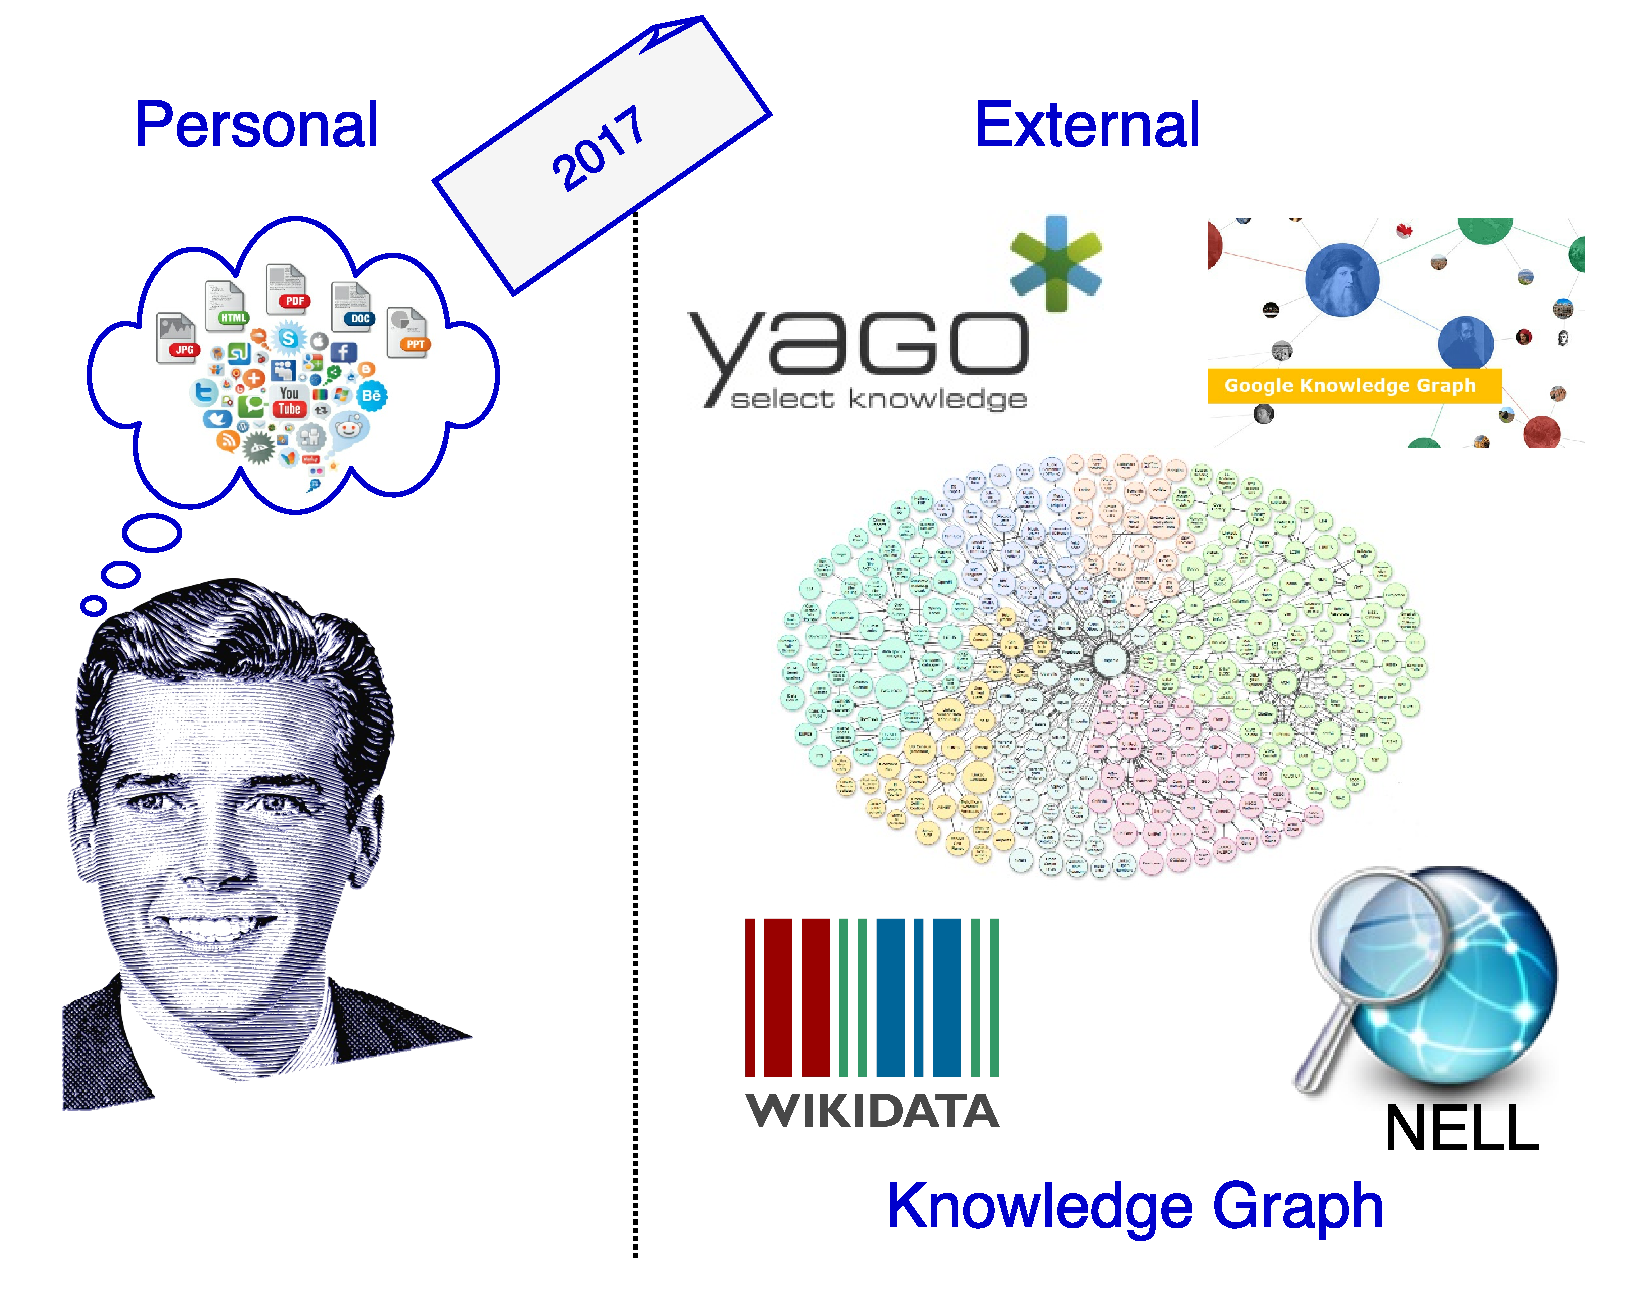
\includegraphics[width=.78\textwidth]{know3_}}
\end{picture}
\end{frame}


\begin{frame}\frametitle{Semantic Web Search}

\alt<3>{\begin{picture}(0.5,0.5)
\put(-13,-135){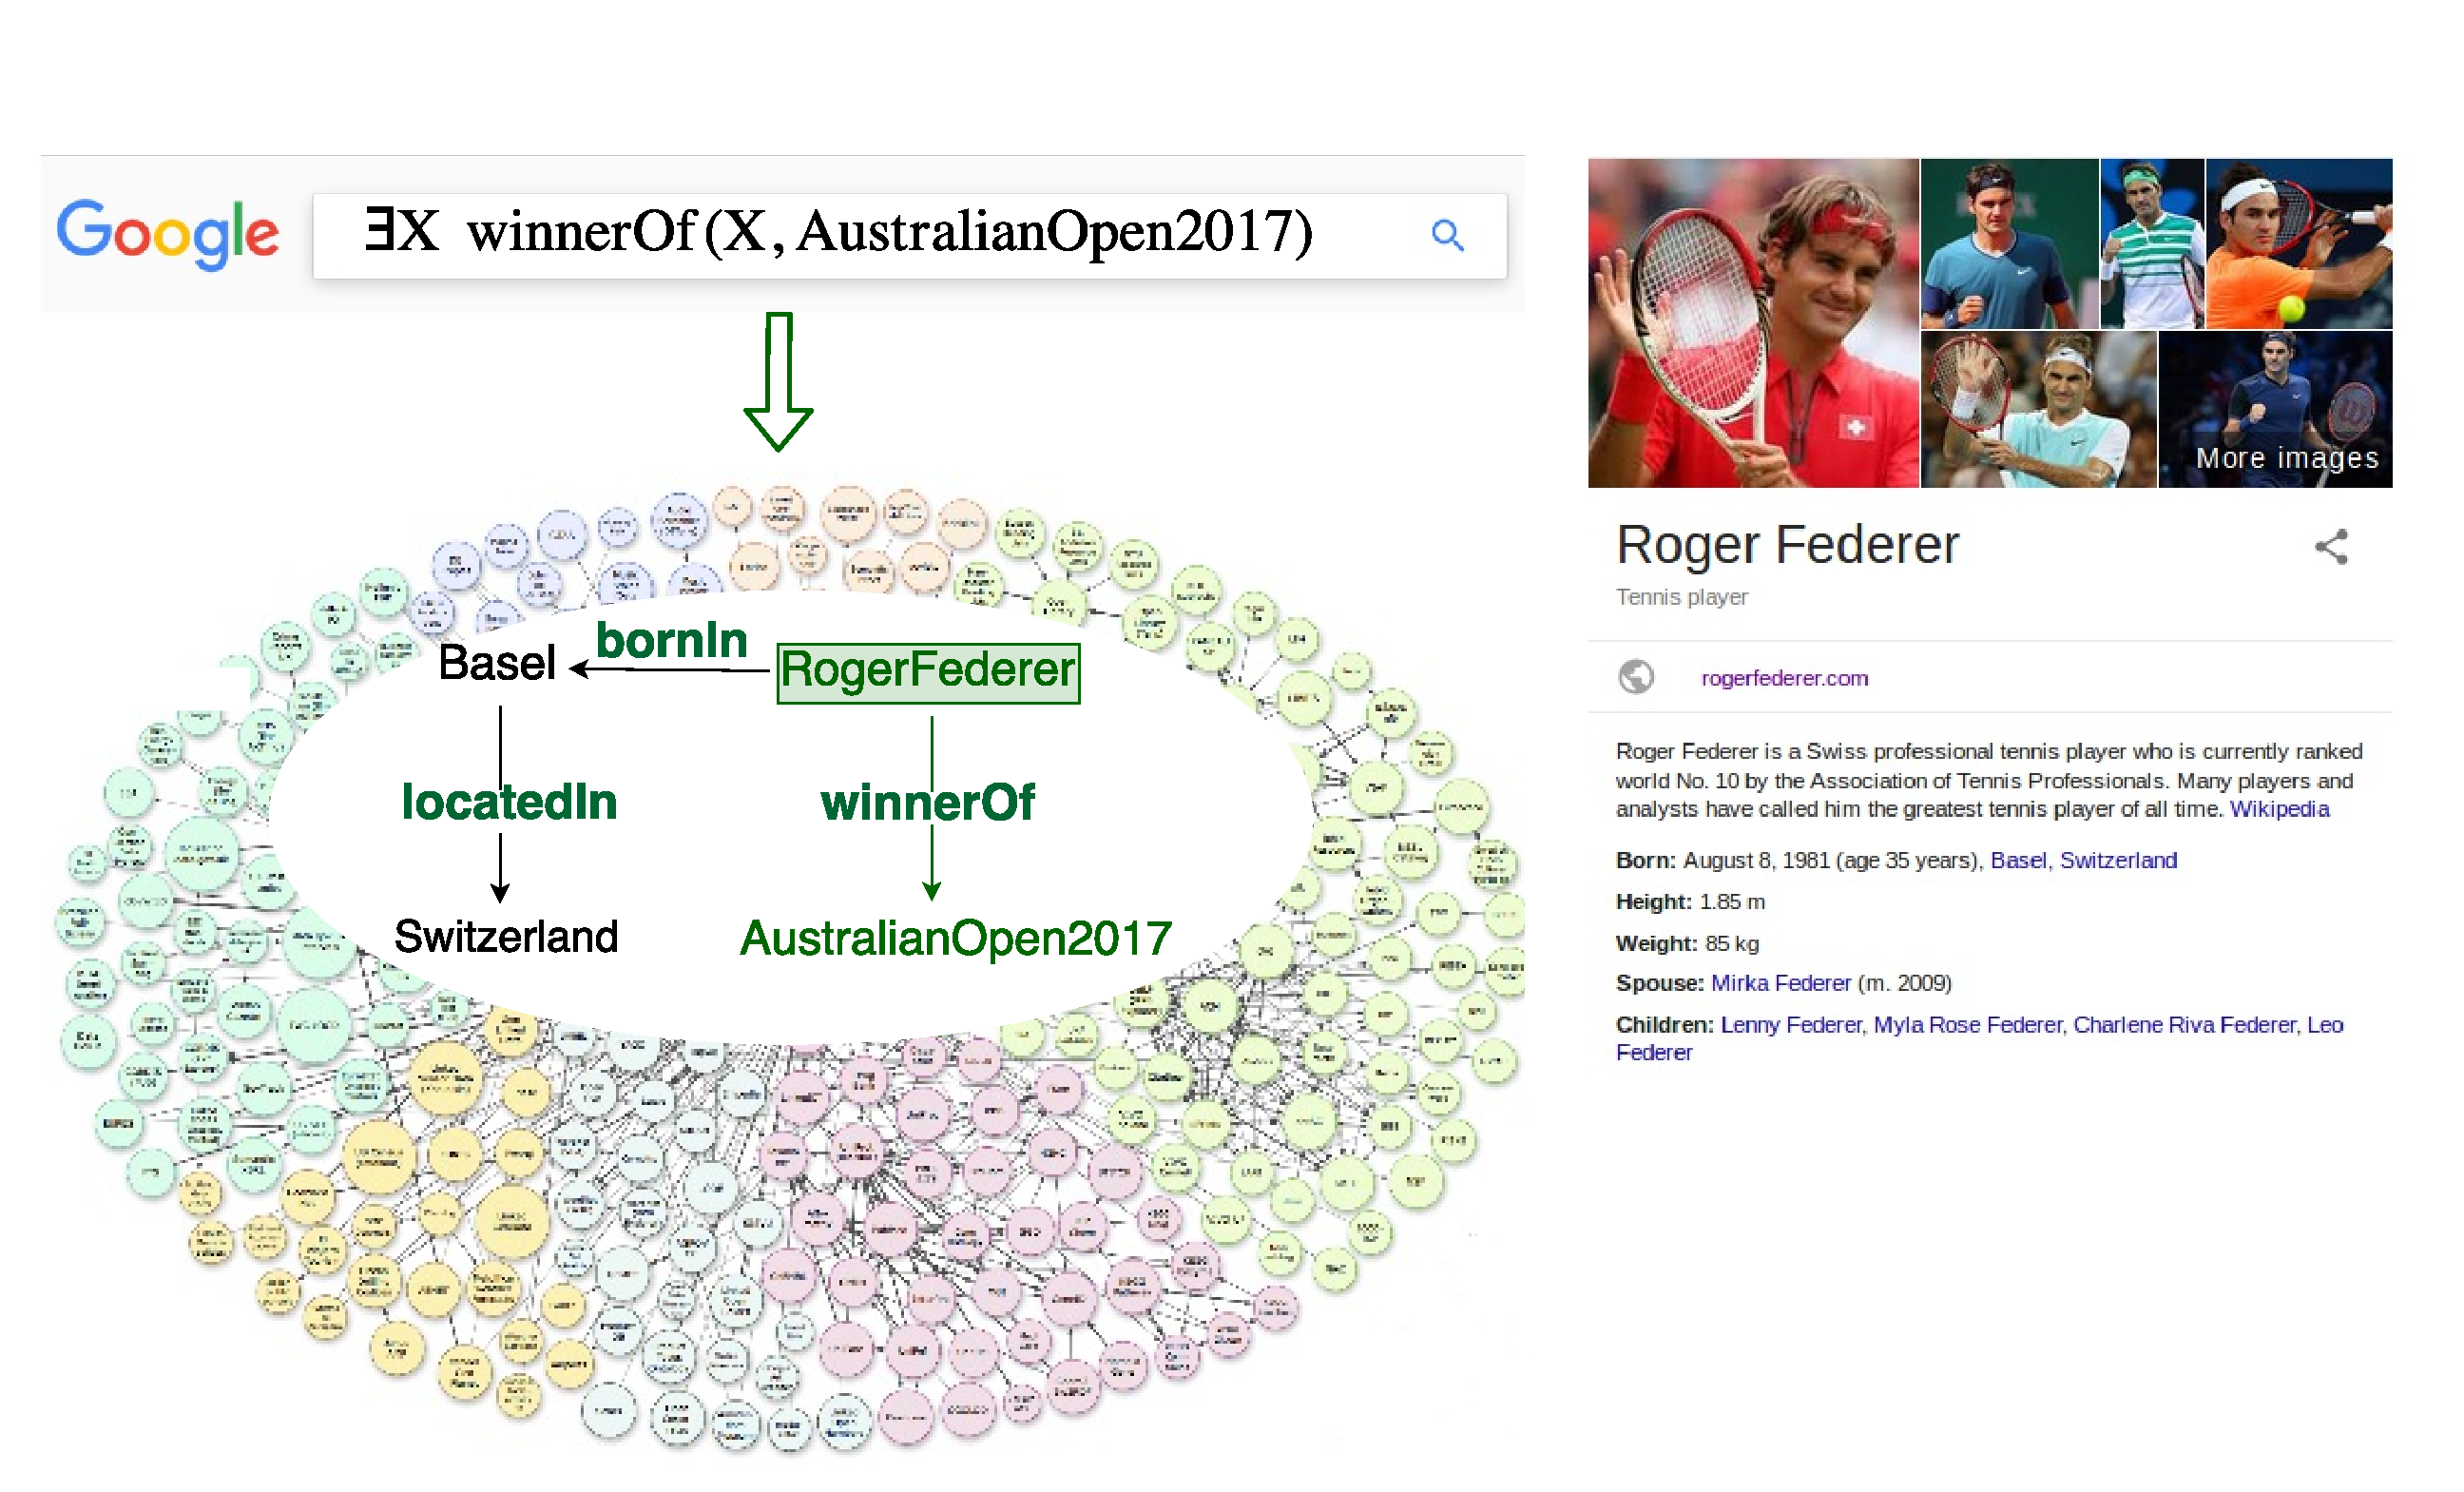
\includegraphics[width=1.1\textwidth]{semsearch3}}
\end{picture}}{
\alt<2>{\begin{picture}(0.5,0.5)
\put(-13,-135){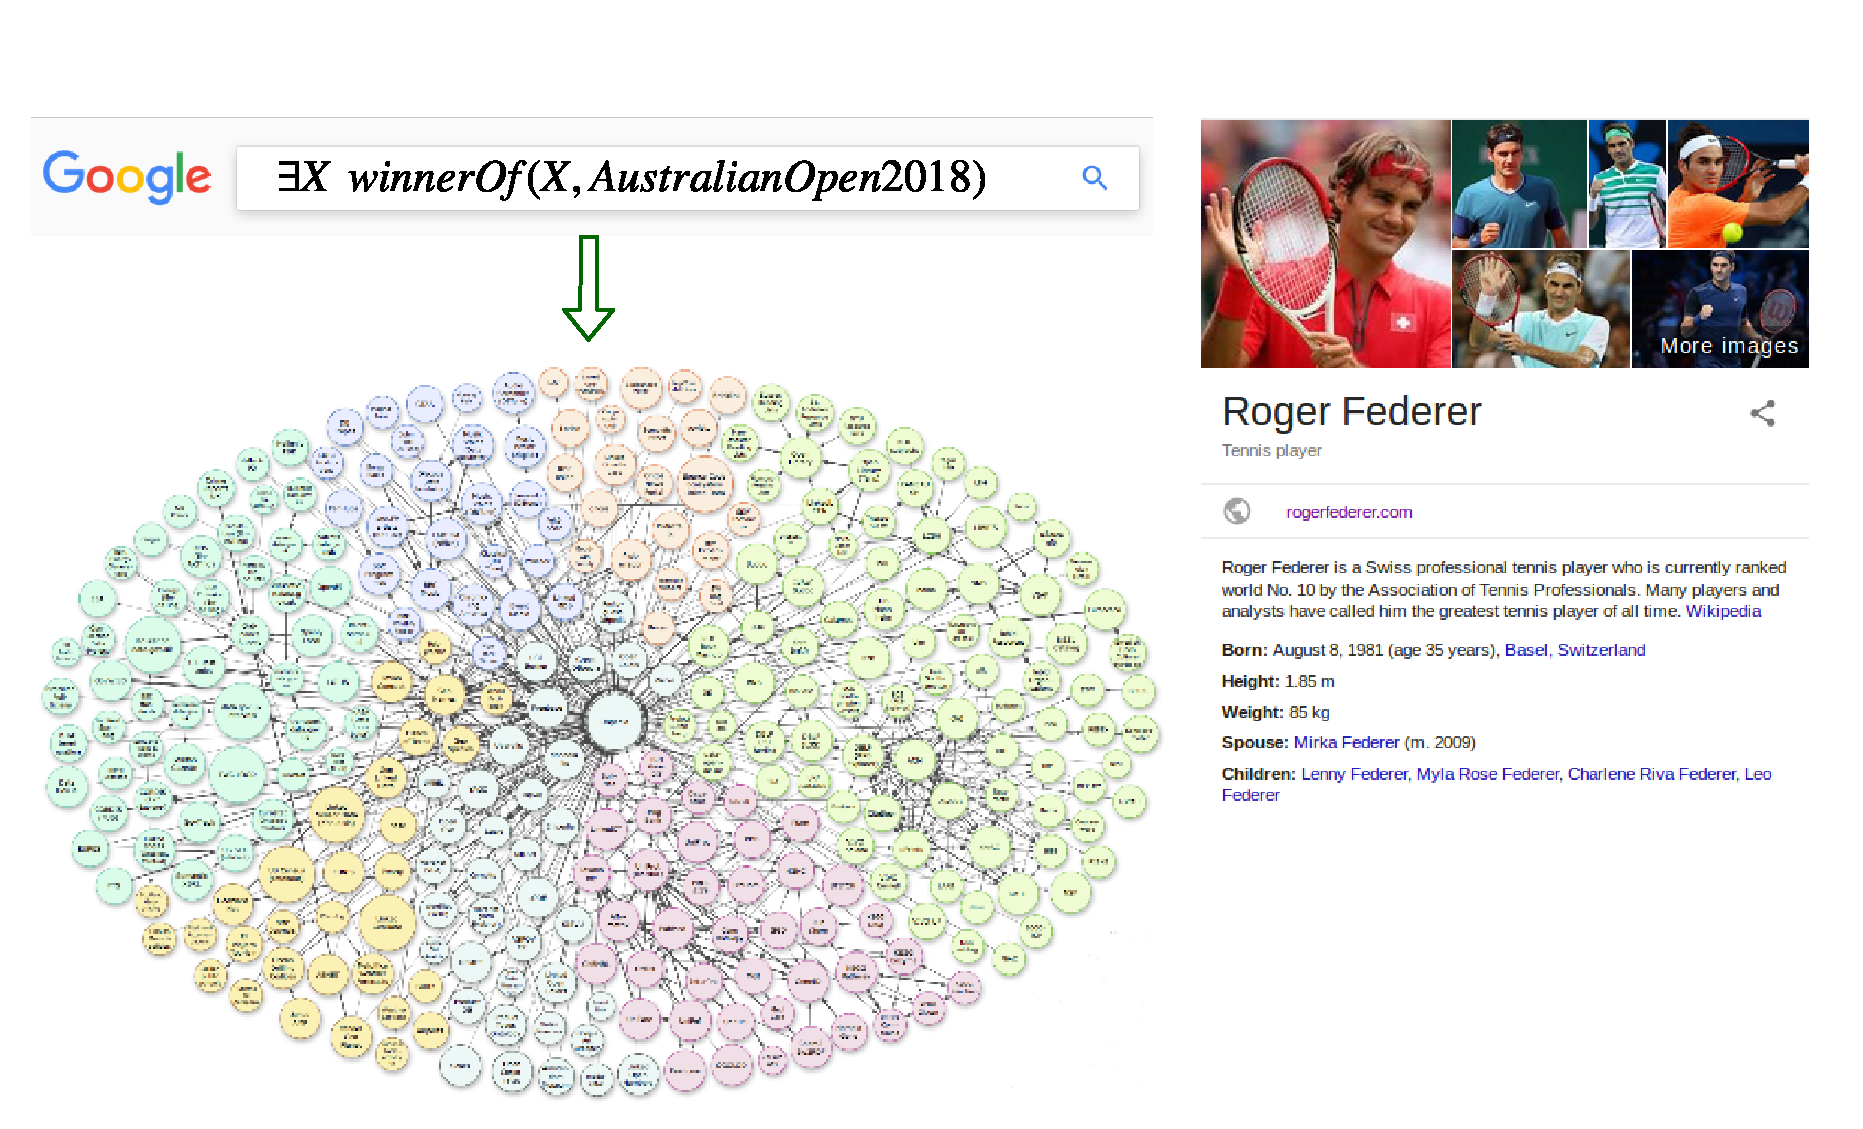
\includegraphics[width=1.1\textwidth]{semsearch2}}
\end{picture}}{
\begin{picture}(0.5,0.5)
\put(-13,-135){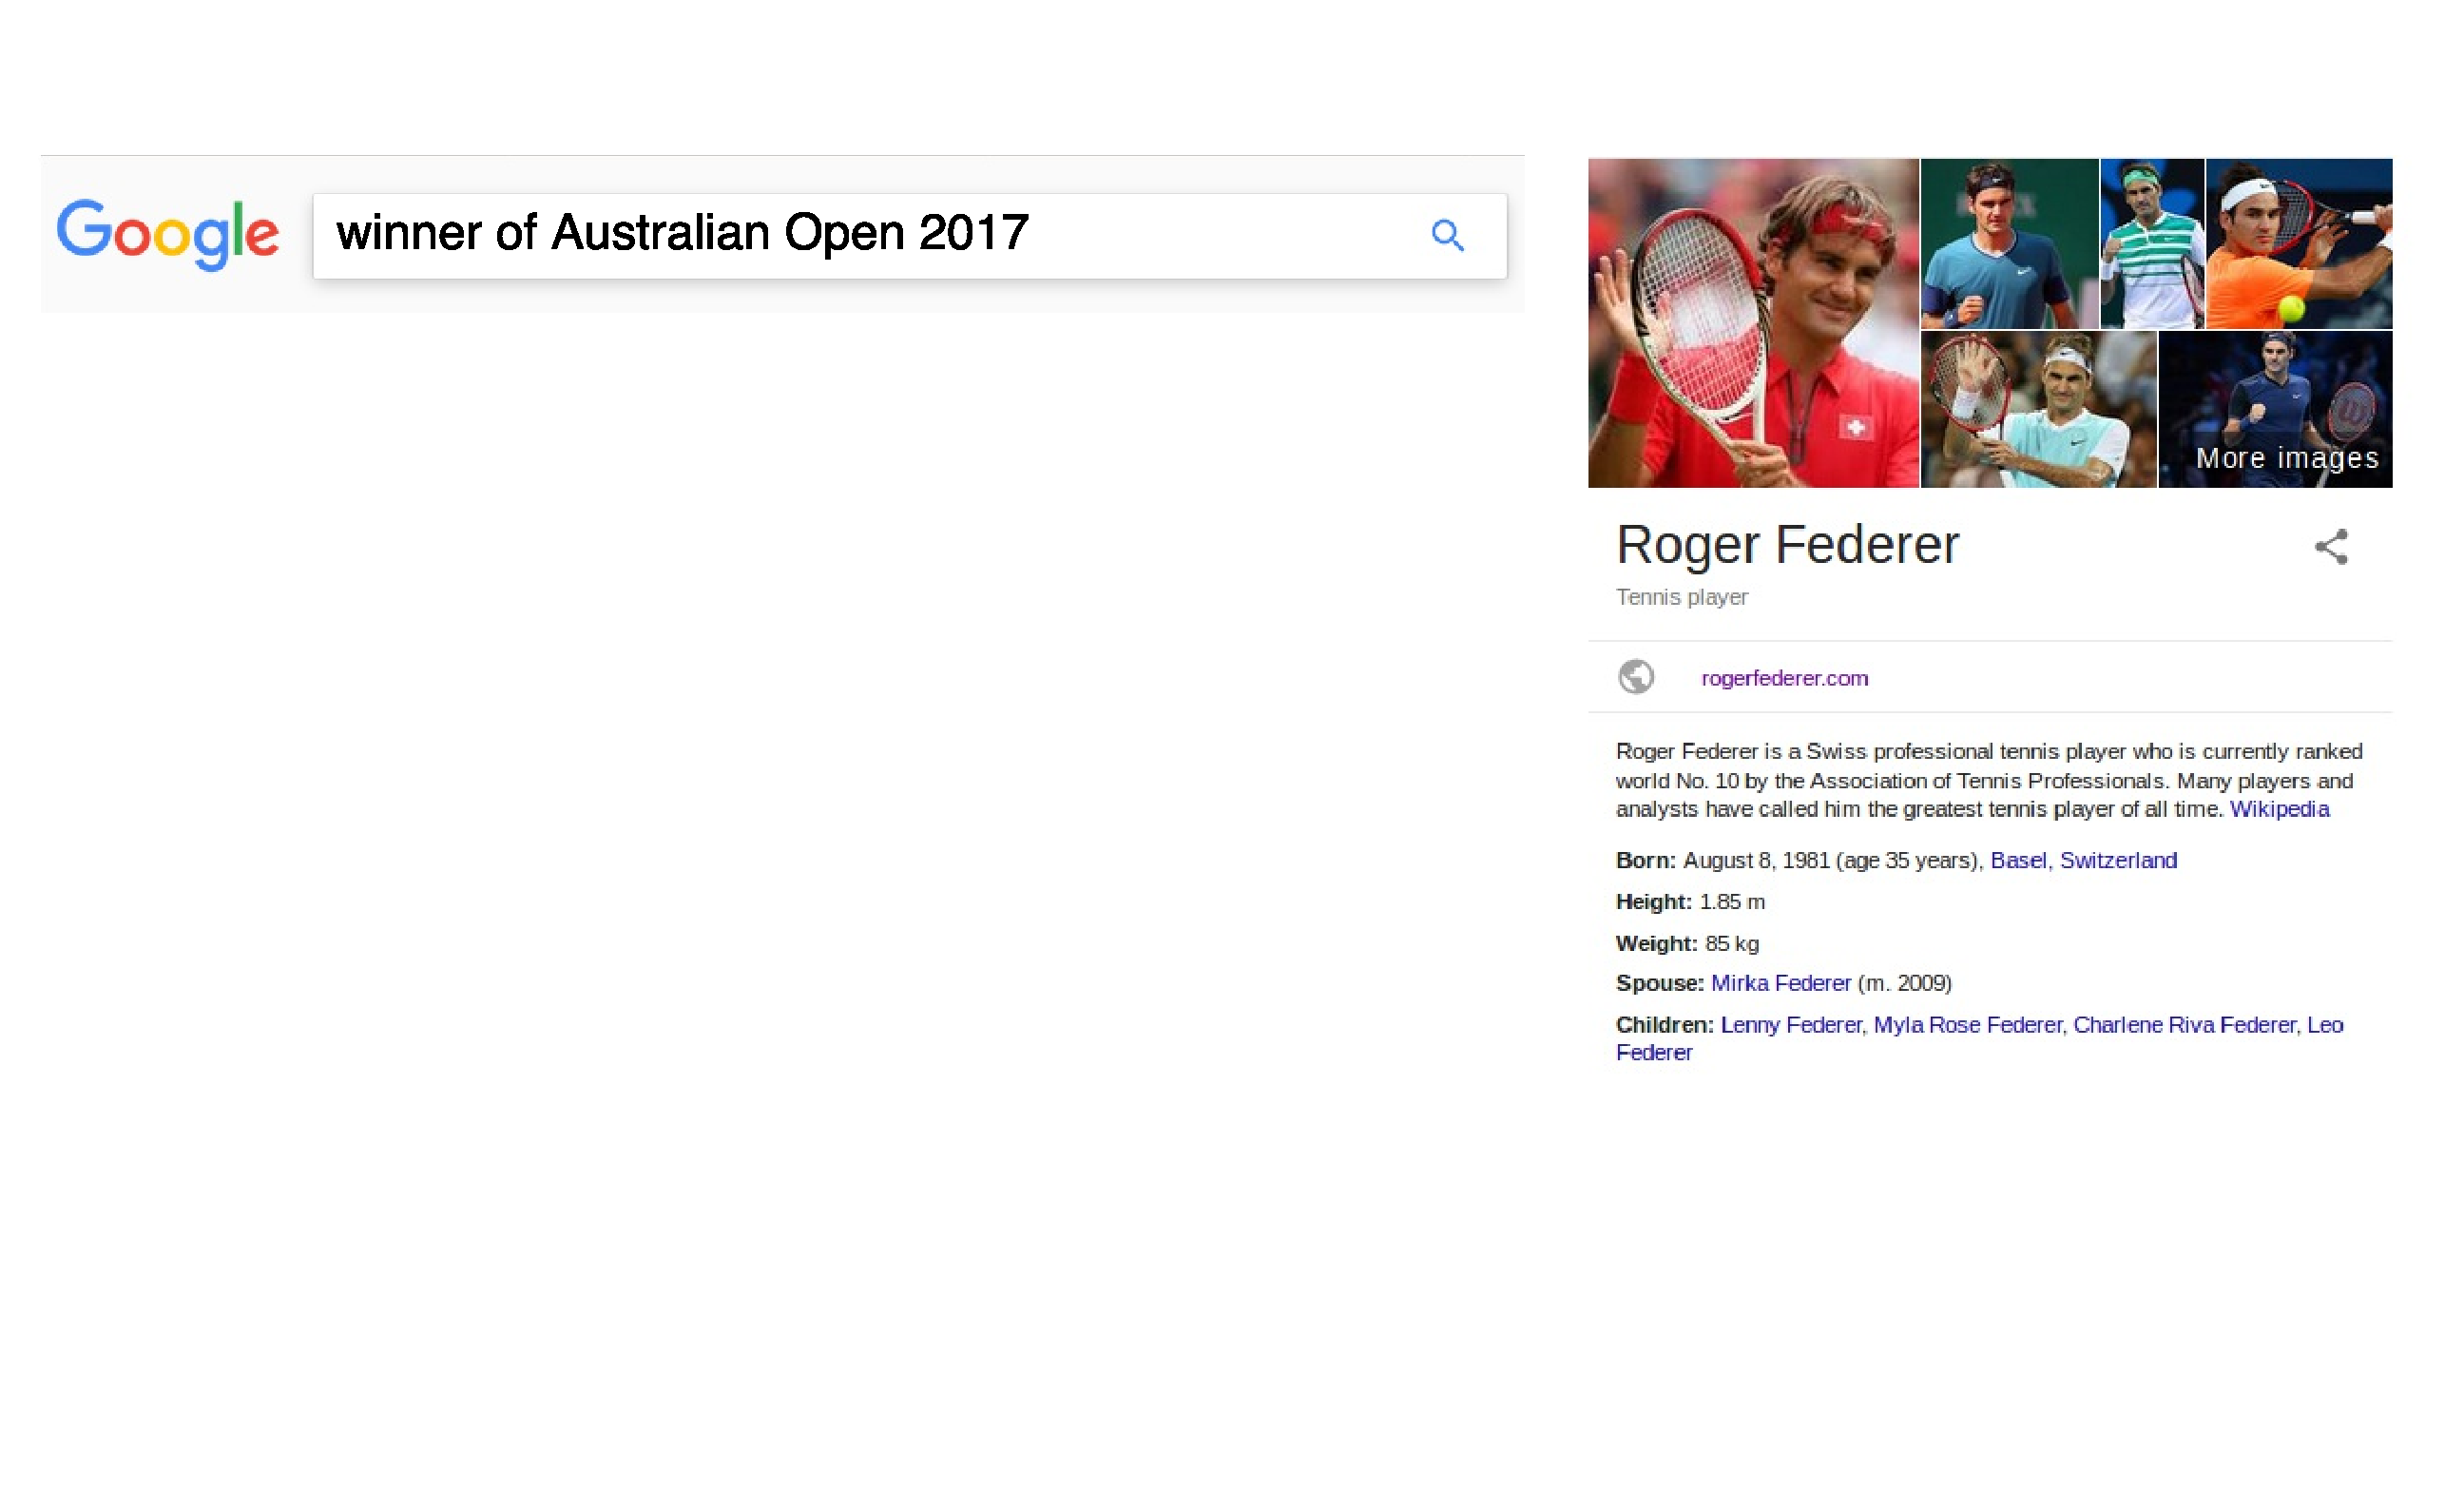
\includegraphics[width=1.1\textwidth]{semsearch1}}
\end{picture}
}}


\end{frame}


% \begin{frame}\frametitle{Knowledge Graphs}
%  \alt<2->{


% \begin{picture}(0.5,0.5)
% \put(217,-130){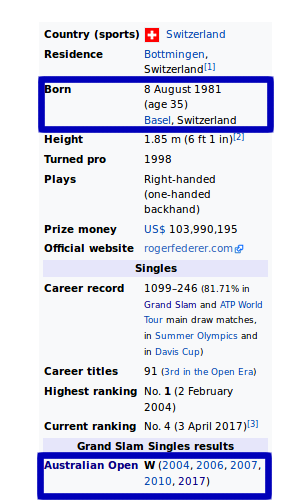
\includegraphics[width=.41\textwidth]{rf_wiki2}}
% \end{picture}
% \begin{picture}(0.5,0.5)
% \put(-5,-120){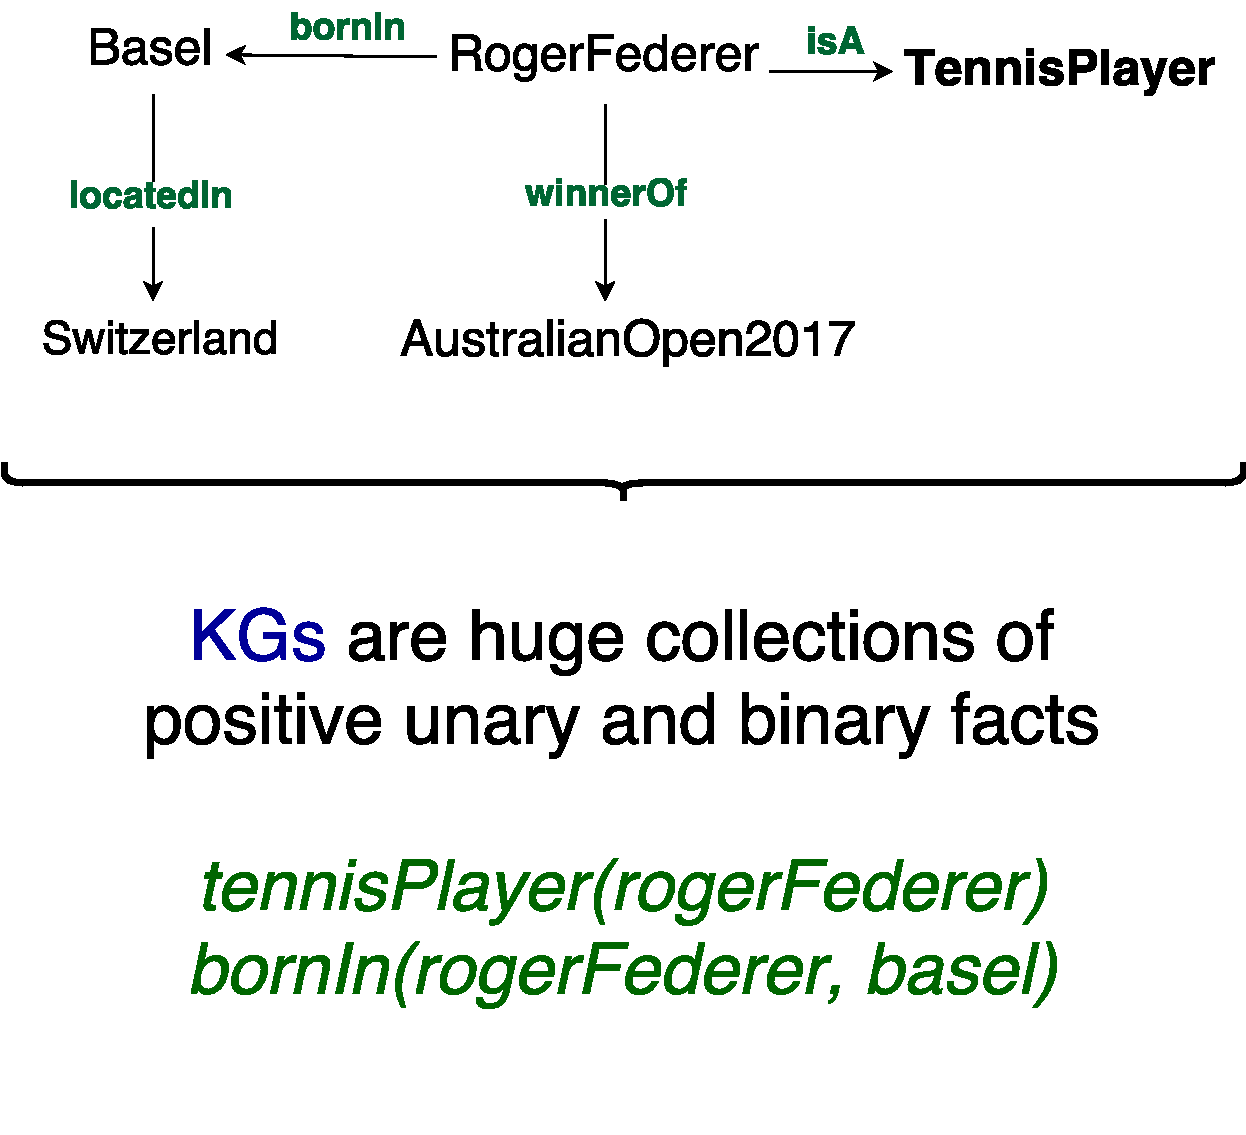
\includegraphics[width=.65\textwidth]{kg_general1}}
% \end{picture}


% }{\begin{picture}(0.5,0.5)
% \put(23,-135){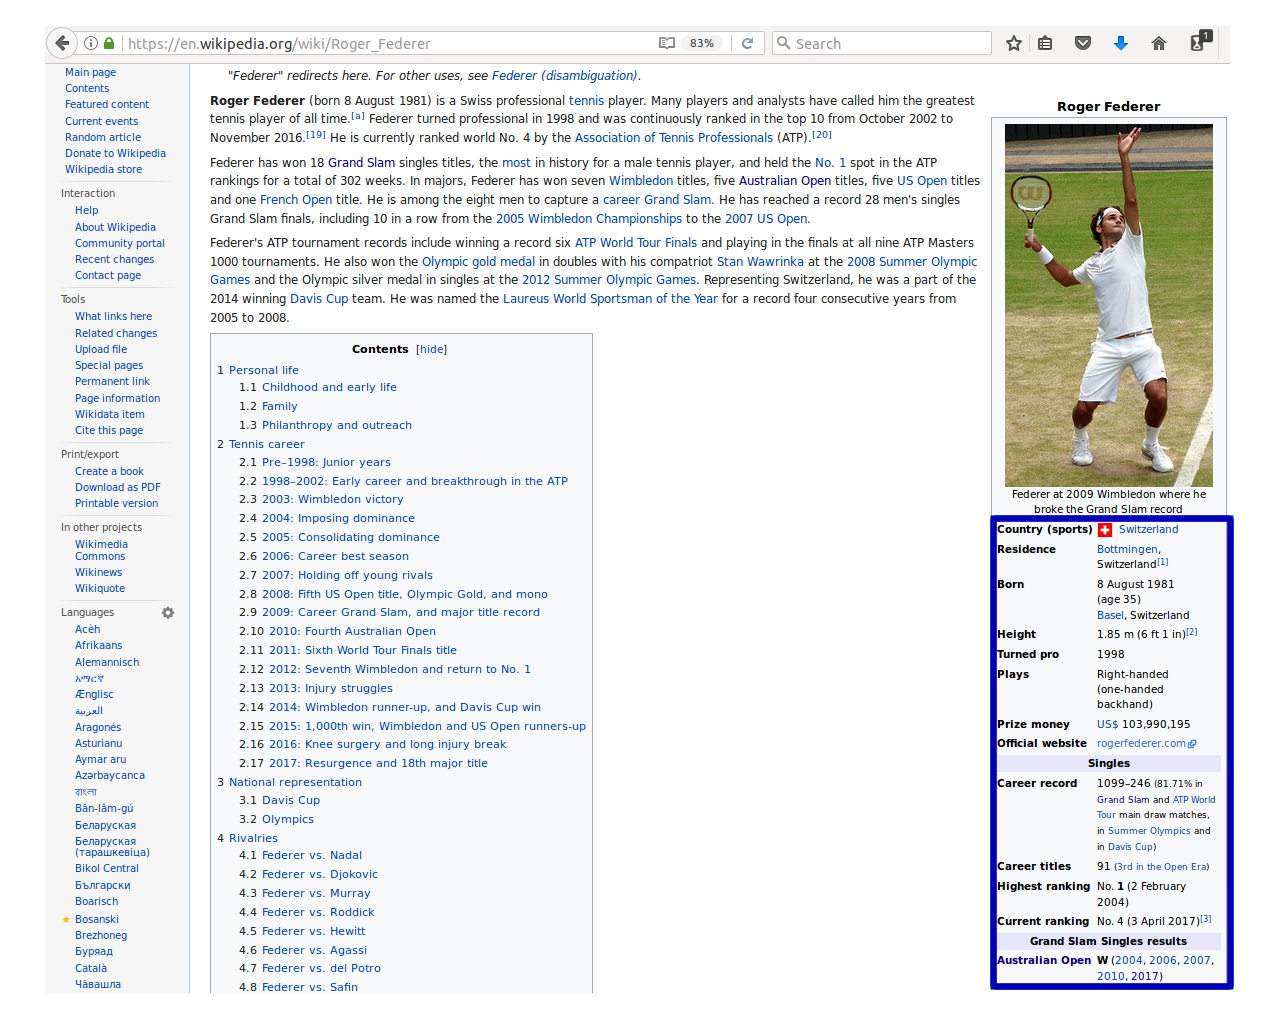
\includegraphics[width=.85\textwidth]{rf_wiki}}
% \end{picture}}
% \end{frame}

\begin{frame}\frametitle{Problem: Inconsistency}
%\alt<2>{
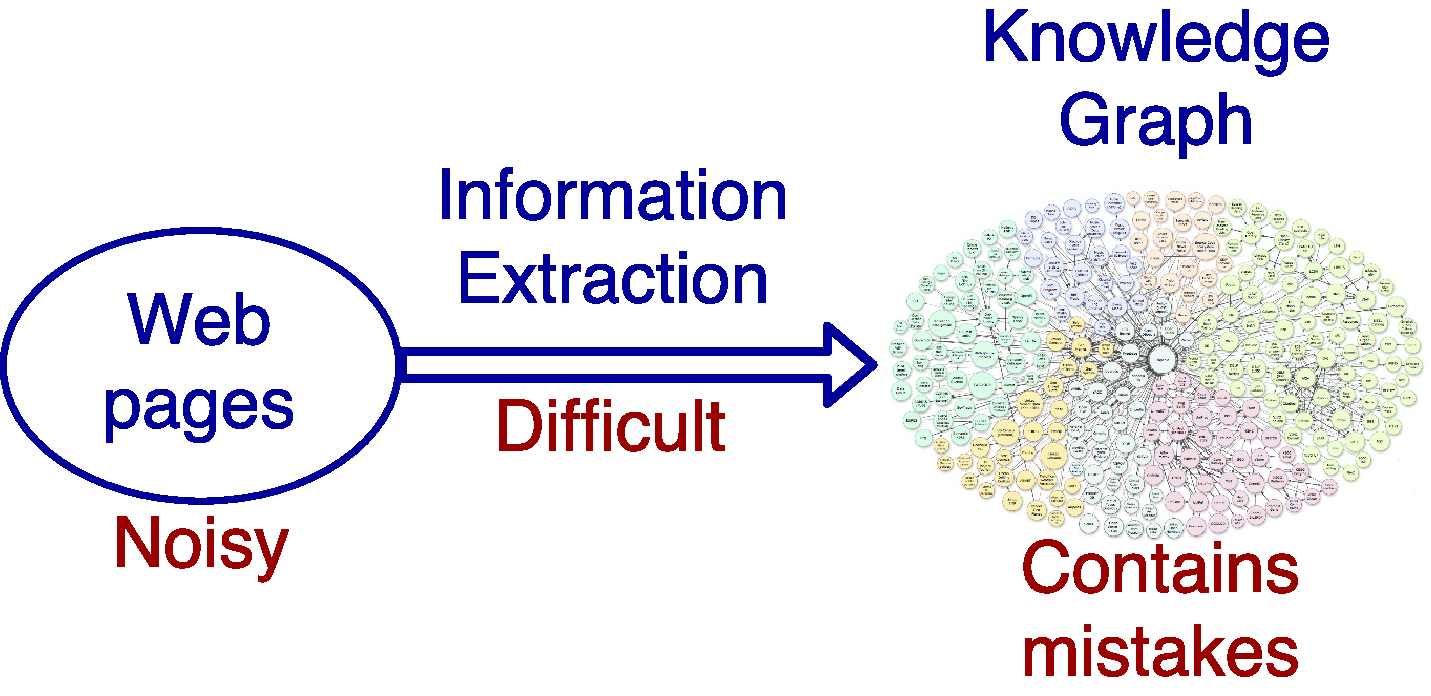
\includegraphics[width=1\textwidth]{kg_problem1}
%}{\includegraphics[width=1\textwidth]{kg_er}}

\end{frame}


\begin{frame}\frametitle{Problem: Incompleteness}
\bigskip

Google KG \alert{misses} Roger's living place, but contains his wife's Mirka's.. 
\bigskip

\begin{center}
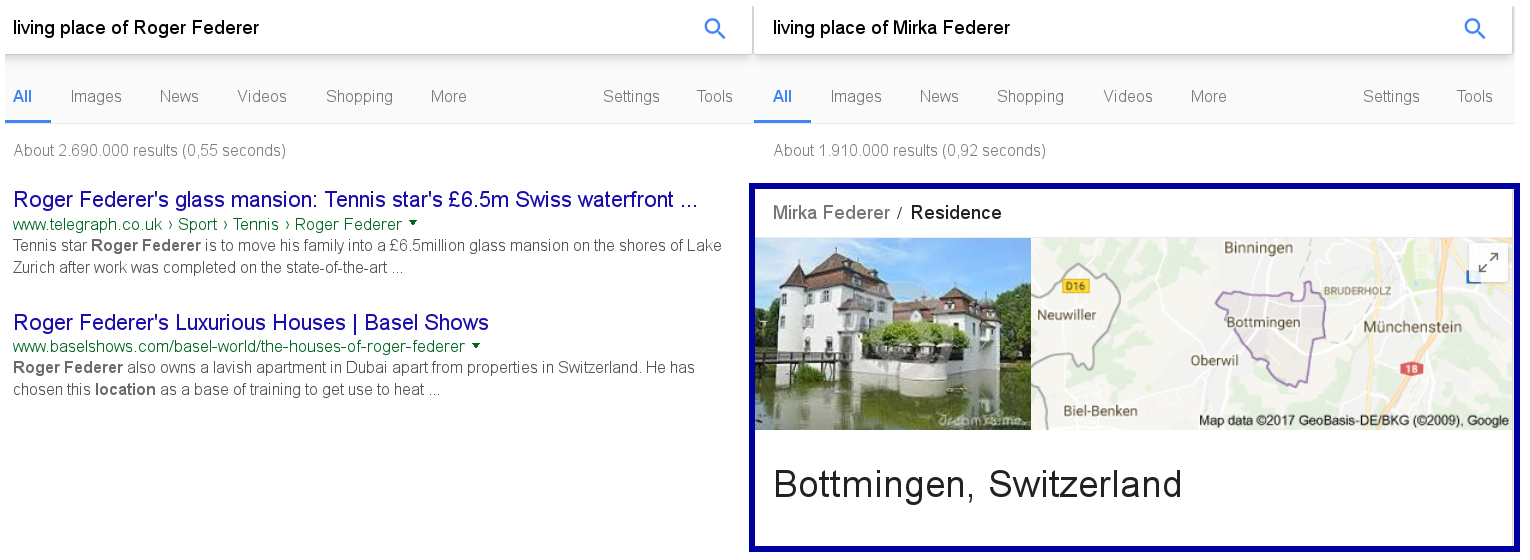
\includegraphics[width=1.02\textwidth]{kg_problem2}
\end{center}
\end{frame}

% \begin{frame}\frametitle{Inconsistency and Incompleteness in KGs}
% \bigskip

% \alt<2>{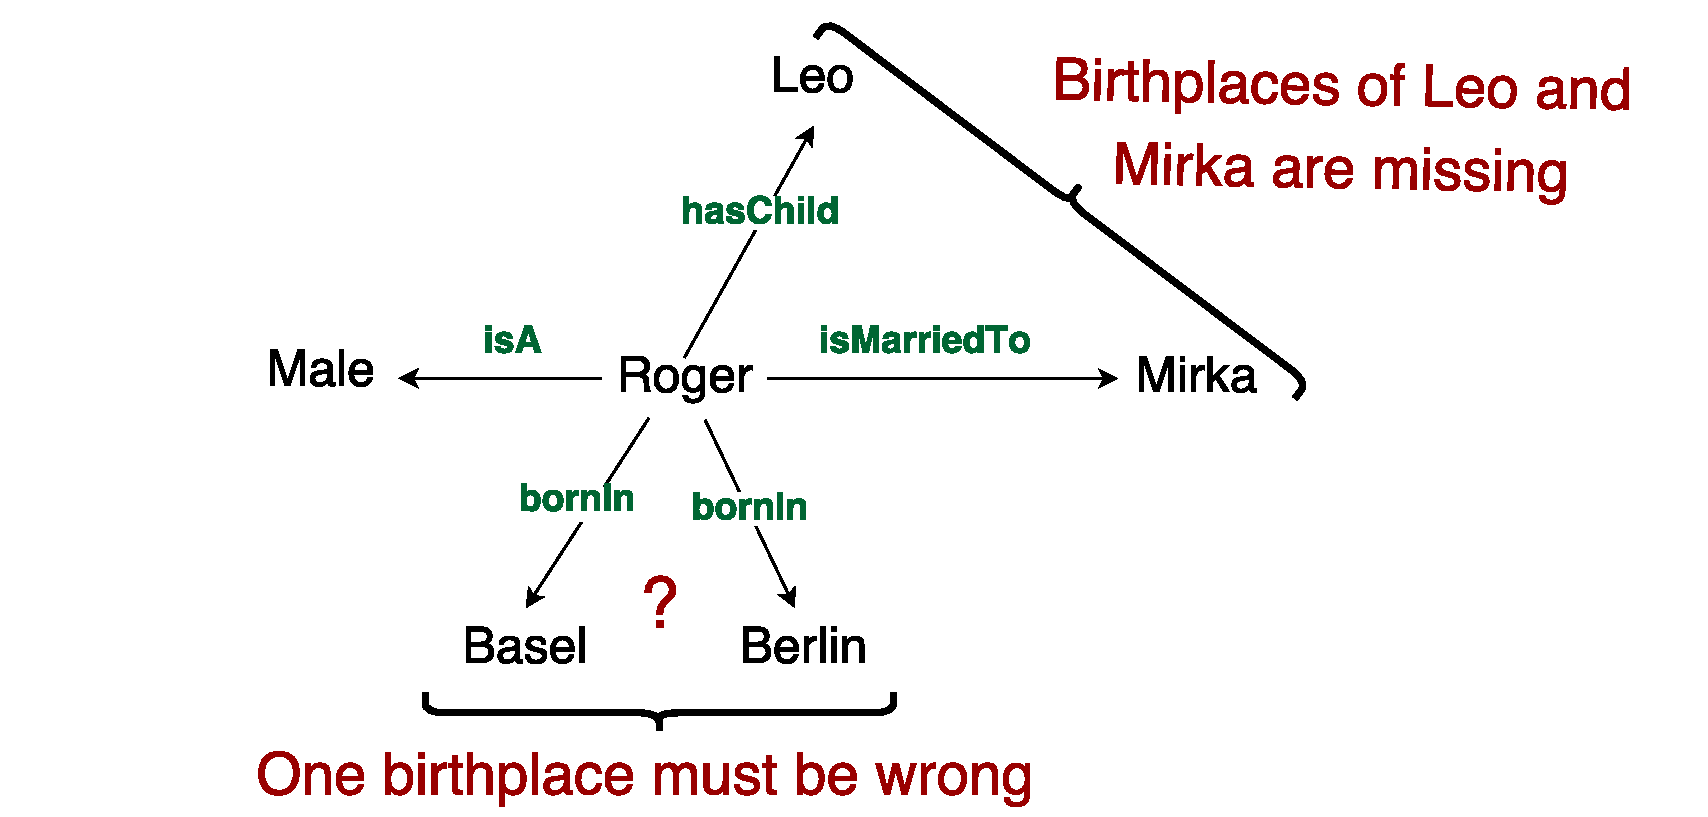
\includegraphics[width=1\textwidth]{kg_inc2}}{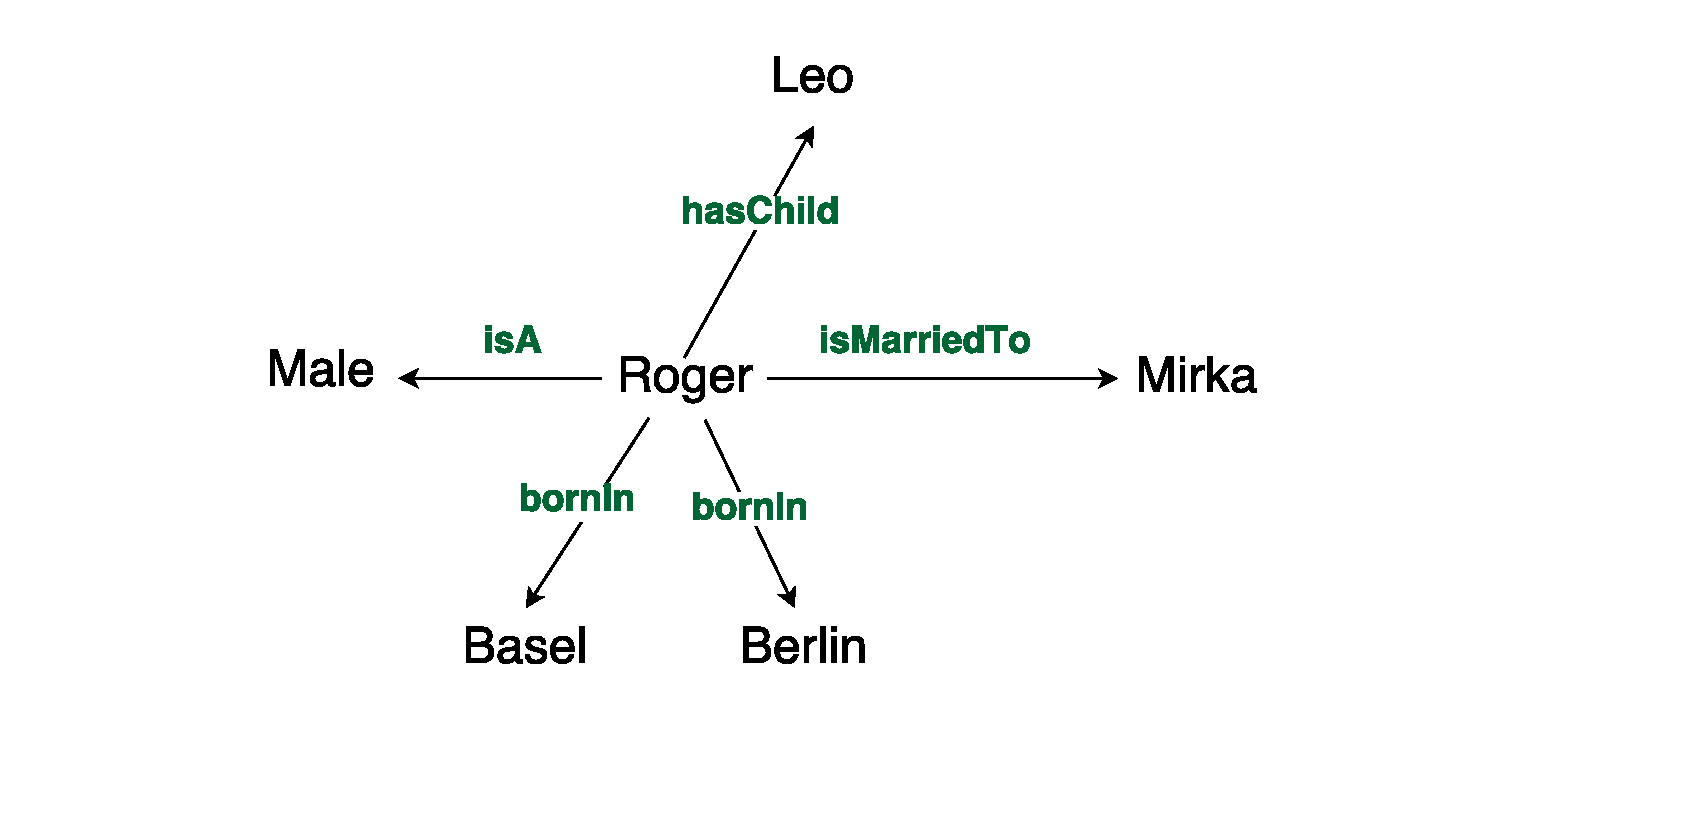
\includegraphics[width=1\textwidth]{kg_inc1}}
% \end{frame}



\begin{frame}\frametitle{What if we had rules?}
\begin{center}
\begin{columns}
\begin{column}{.49\textwidth}
  $\gr{\mi{livesIn(Y,Z)\leftarrow marriedTo(X,Y),}}$ \\
      $\phantom{\mi{livesIn(Y,Z)\leftarrow }}\mi{\gre{livesIn(X,Z)}}$\bigskip

   \uncover<2->{ $\gr{\mi{marriedTo(mirka,roger)}}$\bigskip

  $\gr{\mi{livesIn(mirka, bottmingen)}}$
------------------------------------}\bigskip

  \uncover<3->{\gr{$\mi{livesIn(roger,bottmingen)}$}\bigskip

% 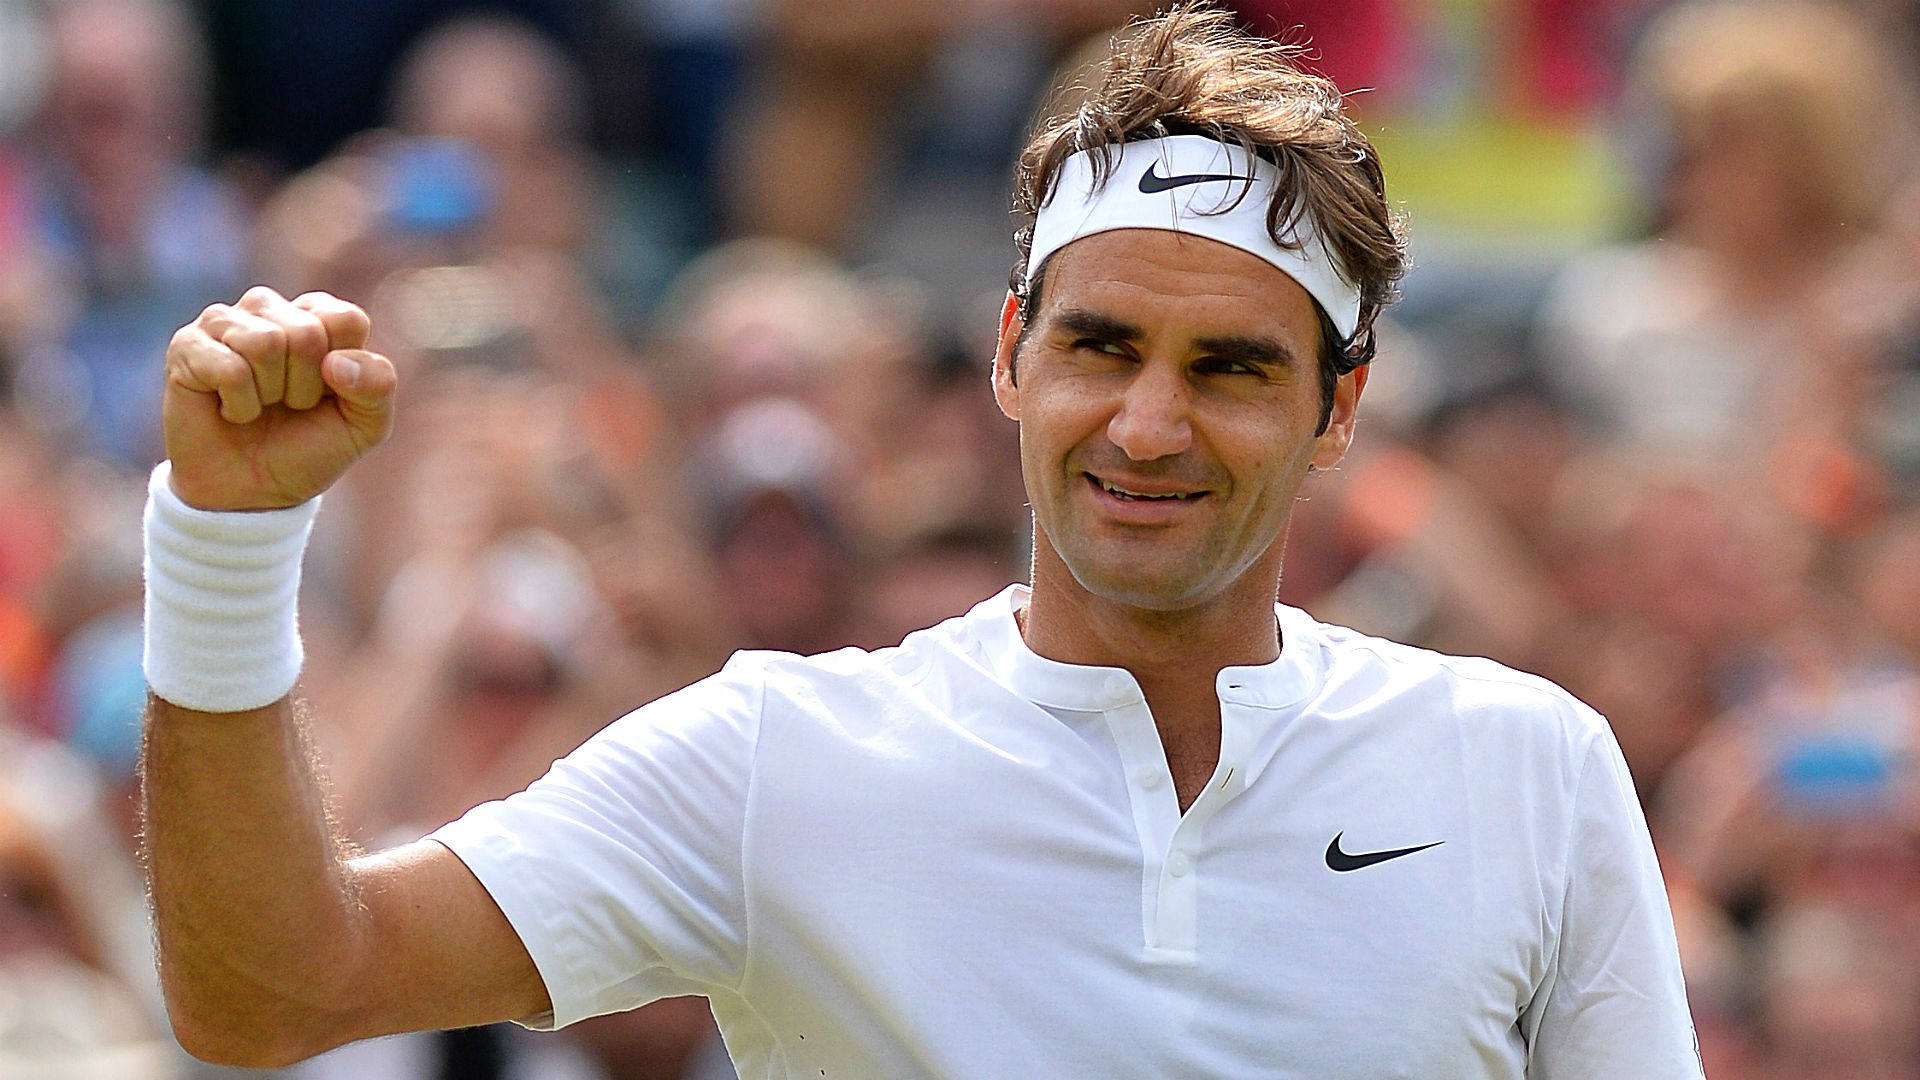
\includegraphics[width=.6\textwidth]{rf_in_bottmingen}
}
\end{column}
\begin{column}{.49\textwidth}

  \emph{Married people live together}\bigskip\bigskip

  \uncover<2->{
  \emph{Mirka is married to Roger}\bigskip\smallskip

  \emph{Mirka lives in Bottmingen}
  \uncover<2->{------------------------------------}\bigskip

}
  \uncover<3->{\emph{Roger lives in Bottmingen} \bigskip

% 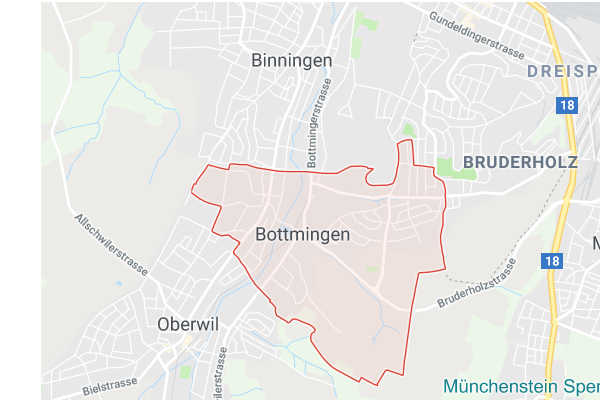
\includegraphics[width=.6\textwidth]{bottmingen}
}
\end{column}
\end{columns}
\includegraphics[width=.6\textwidth]{rogerInBot}
%\begin{picture}(0.5,0.5)
    % \put(50,-136){
%}
   % \end{picture}
\smallskip

\uncover<3->{\alert{But where can one get such rules from?}}
\end{center}
\end{frame}


\begin{frame}\frametitle{Extracting Rules from Knowledge Graphs}
\bigskip
\bigskip
\bigskip
\bigskip
\bigskip
\bigskip
\bigskip
\bigskip
\bigskip
\bigskip

\begin{picture}(0.5,0.5)
\put(43,-35){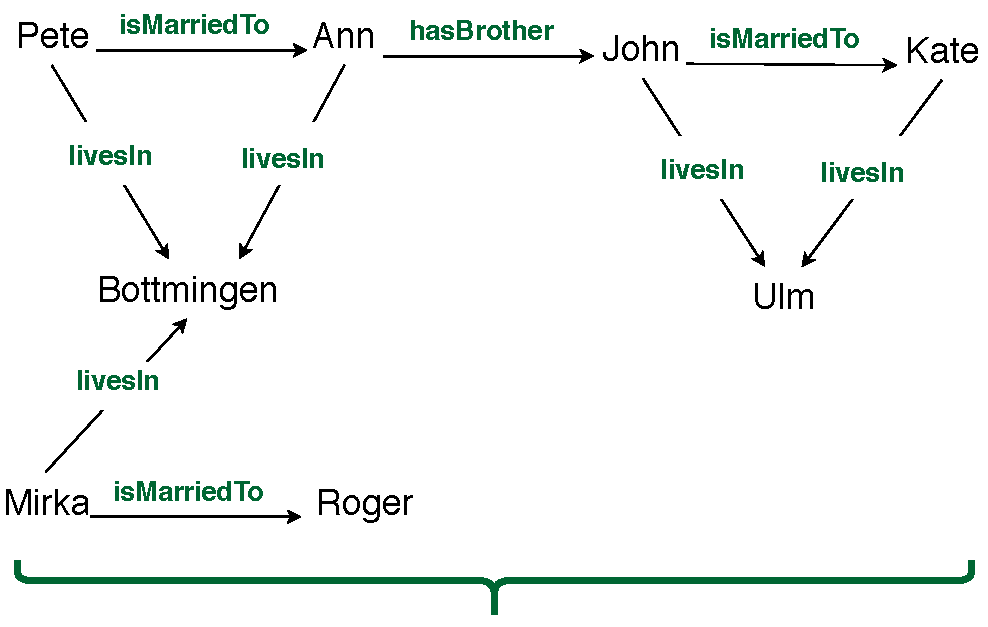
\includegraphics[width=0.75\textwidth]{hr_learn}}
\end{picture}
\bigskip
\bigskip

\begin{center}
\gre{$\mi{livesIn(Y,Z)\leftarrow isMarriedTo(X,Y),livesIn(X,Z)}$}
\end{center}
\end{frame}

\begin{frame}\frametitle{Motivation}
\begin{beamerboxesrounded}[upper=uppercolred,lower=lowercolred,shadow=true]{\textbf{\alert{Important problems}} of KGs:}

 \medskip
 \begin{itemize}
 \item[\alert{\circled{1}}] \alert{Inconsistency} (covered in the morning!)
 \medskip

 \item[\alert{\circled{2}}] \alert{Incompleteness} (focus of this lecture)
 \end{itemize}
 \end{beamerboxesrounded}
\bigskip
\bigskip
\bigskip
\pause 

\begin{beamerboxesrounded}[upper=uppercolblue,lower=lowercolblue,shadow=true]{}
\bigskip

 \begin{itemize}
 \item[] \bl{Inductive learning of common-sense rules for KG completion}
 \end{itemize}
\bigskip

 \end{beamerboxesrounded}
\end{frame}




%\subsection{Knowledge Graphs}

%\section{Horn Rules}

% \frame{\frametitle{}
% \begin{center}
% \bl{\Huge{Horn Logic Programming}}
% \end{center}


% \begin{tikzpicture}[remember picture,overlay]
%     \node[xshift=-90.5mm,yshift=-110,anchor=north east] at (current page.north east){%
%     \includegraphics[width=15mm]{horn}};

% \end{tikzpicture}
% \bigskip
% \bigskip
% \bigskip
% \bigskip
% \bigskip

% $\;\;\;\;\;\;\;\;\;\;\;\;\;$Alfred Horn
% }

%%%%%%%%%%%%%%%%%%%%%%%%%%%%%%%%%%%%%%%%%%%%%%%%%%%%%%%%%%%%%%%%%%%%%%%%%%%%%%


%\subsection{Positive Logic Programs}
% \begin{frame}
% \frametitle{Syntax}


% \bs
% \bi
% \item Assume a vocabulary $\Phi$ comprised of nonempty finite sets of 
% \begin{itemize}
% \item constants (e.g., \gre{$\mi{frankfurt}$})
% \item variables (e.g., \gre{$X$})
% \item predicate symbols (e.g., \gre{$\mi{connected}$})
% \end{itemize}
% \bs
% \pause

% \item A \bl{term} is either a variable, a constant, or inductively built from other terms using function symbols.
% \bs
% \pause

% \item An \bl{atom} is an expression of form \bl{$p(t_1,\ldots{},t_n)$}, where 


% \bi
% \item \bl{$p$} is a \bl{predicate symbol} of \bl{arity $n \ge 0$} from $\Phi$, and 
% \item \bl{$t_1,\ldots{},t_n$} are terms. 
% \ei
% (e.g., \gre{$\mi{connected(frankfurt)}$})
% \bs
% \pause

% \item A \bl{term} or an \bl{atom} is \emph{ground} if it contains no variable.\\
% (e.g., \gre{$\mi{connected(frankfurt)}$ is ground}, \gre{$\mi{connected(X)}$} is nonground.)
% \end{itemize}

% \end{frame}

%%%%%%%%%%%%%%%%%%%%%%%%%%%%%%%%%%%%%%%%%%%%%%%%%%%%%%%%%%%%%%%%%%



%%%%%%%%%%%%%%%%%%%%%%%%%%%%%%%%%%%%%%%%%%%%%%%%%%%%%%%%%%%%%%%%%%

\section{Preliminaries}
\subsection{Horn Rules}
\begin{frame}
  \frametitle{Horn Rules}
\bigskip

\small{ \bl{\textbf{Rule:} }
$\underbrace{a}_{\Large{\bl{\text{head}}}}\; \leftarrow\; \underbrace{b_1,\, \dotsc,\, b_m.}_{\bl{\text{body}}} $

\bigskip
\bigskip

\small{\bl{\textbf{Informal semantics:}} } If $b_1,\dotsc, b_{m}$ are true, then $a$ must be true.\bigskip
\bigskip

\small{\bl{\textbf{Logic program:}} } Set of rules 

%\small{\bl{\textbf{Closed World Assumption (CWA):} }} facts not known to be true are false
\bigskip
\bigskip

}
\begin{beamerboxesrounded}[upper=uppercolgreen,lower=lowercolgreen,shadow=true]{\alt<2->{Example: non-ground rule}{Example: ground rule}}
\medskip
\small{
\alt<2->{\gre{\%\,Married people live together}\\
$\mi{livesIn(Y,Z)}\leftarrow\mi{isMarried(X,Y)}, \mi{livesIn(X,Z)}$
\bigskip
\bigskip

% \gre{\%\,Constraint: ensure that none is a parent of himself}\\
% $ \bot \leftarrow \mi{parent(X,Y),parent(Y,X)}$
}{\gre{\%\,If Mirka is married to Roger and lives in B., then Roger lives there too}\\
$\mi{livesIn(roger,bottmingen)}\leftarrow\mi{isMarried(mirka,roger)}, \mi{livesIn(mirka,bottmingen)}$
\bigskip

% \gre{\%\,Constraint: It cannot be the case that Roger is a parent of Leo and vice versa }\\
% $ \bot \leftarrow \mi{parent(roger,leo),parent(leo,roger)}$
}}
\end{beamerboxesrounded}

\bigskip



\end{frame}


% \begin{frame}
% \frametitle{Horn Rules}


% %%\normalsize

% \begin{beamerboxesrounded}[upper=uppercolblue,lower=lowercolblue,shadow=true]{Def.: \textbf{Horn rule}}
% A \bl{Horn rules} $r$ is an expression of the form
% %
% %
% \begin{equation}
%  \label{eq:clause}
%  \bl{a \leftarrow b_1,\ldots,b_m,}
% \end{equation}
% %
% where $a$, $b_1$, \ldots, $b_m$ are atoms.
% %  of a first-order language $L$.
% \begin{itemize}
%             \item  $a$ is the \bl{head} of the rule
%             \item  $b_1,\ldots,b_m$ is the  \bl{body} of the rule.
% \item
% If $m=0$, the rule is a \bl{fact} (written shortly $a$)
% \end{itemize}
% \end{beamerboxesrounded}

% \bs
% % \begin{beamerboxesrounded}[upper=uppercolgreen,lower=lowercolgreen,shadow=true]{Example:}
% % Ground rule: \gre{$$}
% % \end{beamerboxesrounded}

% Intuitively, (\ref{eq:clause}) can be seen as material implication
% \begin{center}
% \bl{$\forall \vec{x}\; b_1\land\cdots\land b_m \rightarrow a$}, where \bl{$\vec{x}$}
% \end{center}
% is the list of all variables occurring in (\ref{eq:clause}).

% \end{frame}

% %%%%%%%%%%%%%%%%%%%%%%%%%%%%%%%%%%%%%%%%%%%%%%%%%%%%%%%%%%%%%%%%%%



\begin{frame}
\frametitle{Herbrand Semantics}

{\small
\medskip

%\begin{beamerboxesrounded}[upper=uppercolblue,lower=lowercolblue,shadow=true]{Def.: \textbf{Herbrand universe, base, interpretation}}

%\small
\textbf{\bl{Herbrand universe}} of a logic program $P$, $\bl{HU(P)}$ is the  set of all constants appearing in $P$
\bs

\textbf{\bl{Herbrand base}} of $P$, \bl{$\HB(P)$} is the set of all ground
atoms which can be formed from predicates and constants of $P$.
\pause

\bs
\textbf{\bl{(Herbrand) interpretation}} of $P$, \bl{$I$} is a subset of the Herbrand base.

%\end{beamerboxesrounded}
\bs



\begin{beamerboxesrounded}[upper=uppercolgreen,lower=lowercolgreen,shadow=true]{Example: Herbrand universe, base, interpretation}
\medskip

$P=\{isMarriedTo(mirka, roger), livesIn(mirka, bottmingen),$ \s

$\phantom{P=\{}livesIn(Y,Z)\leftarrow isMarriedTo(X,Y), livesIn(X,Y)\}$\s

 $\mi{HU(P)=mirka,roger,bottmingen}$\s

 $\mi{HB(P)=\{isMarriedTo(mirka,mirka),isMarriedTo(mirka,roger),\dotsc}$\\$\phantom{HB(P)=\{}\mi{livesIn(mirka,bottmingen),livesIn(roger,bottmingen),\dotsc\}}$\s

 $I_1=\emptyset, I_2=\{\mi{isMarriedTo(mirka, roger),livesIn(bottmingen,bottmingen)}\}, \dotsc$

\end{beamerboxesrounded}

}


\end{frame}

%%%%%%%%%%%%%%%%%%%%%%%%%%%%%%%%%%%%%%%%%%%%%%%%%%%%%%%%%%%%%%%%%%%%5

% \begin{frame}
% \frametitle{Example}

% % \begin{example}[Program $P_1$]

% % \nbls

% \ms
% \begin{beamerboxesrounded}[upper=uppercolgreen,lower=lowercolgreen,shadow=true]{}

% Program $P$:
% {\small
% \begin{align*}
% \gre{p(X,Y,Z)   \implied  p(X,Y,Z'), h(X,Y), t(Z,Z',r).} \\
% \gre{h(X,Z')  \implied p(X,Y,Z'), h(X,Y), t(Z,Z',r).} \\
%               \gre{p(0,0,b).} \qquad \gre{h(0,0).} \qquad  \gre{t(a,b,r). }
% \end{align*}
% }

% \nbls
% \pause

% \bi
% \item
%  Constant symbols: \gre{$0$, $a$, $b$,  $r$.}%;\; \qquad 

% % \bigskip
% \pause

% \item
% Herbrand universe $\HU(P)$: \qquad \gre{$\{ 0, a, b, r\}$}\pause
% % \bs
% %
% \item ~\\[-0.8\baselineskip]
% $\begin{array}{@{}r@{~}l}
% \text{Herbrand base }\HB(P): \qquad \gre{\{} & \gre{p(0,0,0), p(0,0,a), \ldots , p(r,r,r),}\\ 
%                     & \gre{h(0,0), h(0,a), \ldots,  h(r,r,r),} \\
%                     & \gre{t(0,0,0), t(0,0,a), \ldots ,t(r,r,r) \}}
% \end{array}
% $

% \ms
% \pause

% \item
% Some Herbrand interpretations:

% \s

% \qquad \gre{$I_1 = \emptyset$;~ \quad $I_2 = \HB(P)$;~\quad $I_3 = \{ h(0,0), t(a,b,r),
% p(0,0,b)\}$.}%; \ldots
% % \end{example}
% \ei
% \end{beamerboxesrounded}
% \end{frame}



%%%%%%%%%%%%%%%%%%%%%%%%%%%%%%%%%%%%%%%%%%%%%%%%%%%%%%%%%%%%%%%%%%5

\begin{frame}
\frametitle{Grounding Example}

% \begin{example}[Program $P_2$]
\begin{beamerboxesrounded}[upper=uppercolgreen,lower=lowercolgreen,shadow=true]{}

Program $P$:
{\small
\begin{align*}
\gre{p(X,Y,Z)   \implied  p(X,Y,Z'), h(X,Y), t(Z,Z',r).} \\
\gre{h(X,Z')  \implied p(X,Y,Z'), h(X,Y), t(Z,Z',r).} \\
              \gre{p(0,0,b).} \qquad \gre{h(0,0).} \qquad  \gre{t(a,b,r). }
\end{align*}
}

\nbls
\pause

\bi
\item
The ground instances of the first rule are
\ei
%
{\small\begin{align*}
\gre{p(0,0,0)} &\gre{\implied  p(0,0,0), h(0,0), t(0,0,r).} & \gre{X=Y=Z=Z'=0 }\\
 &\ \ \ \gre{\ldots} \\
\gre{p(0,r,0)} &\gre{\implied  p(0,r,0), h(0,r), t(0,0,r).} & \gre{X=Z=Z'=0, Y=r} \\
 &\ \ \ \gre{\ldots} \\
\gre{p(r,r,r)} &\gre{\implied  p(r,r,r), h(r,r), t(r,r,r).} & \gre{X=Y=Z=Z'=r} \\
 \end{align*}}
 
 \hnbls

\vspace{-2em}
\bi
\item
The single ground instance of the last rule is
{\small\begin{align*}
\gre{t(a,b,r)}
\end{align*}}
%\end{example}

\ei

\end{beamerboxesrounded}
\end{frame}

%%%%%%%%%%%%%%%%%%%%%%%%%%%%%%%%%%%%%%%%%%%%%%%%%%%%%%%%%%%%%%%%%

\begin{frame}
\frametitle{Herbrand Models}

\begin{beamerboxesrounded}[upper=uppercolblue,lower=lowercolblue,shadow=true]{Def.: \bl{\textbf{Herbrand models}}}
\bs

An interpretation $I$ is a \bl{(Herbrand) model} of

\begin{itemize}
\item \bl{a ground (variable-free) clause $C = a \implied b_1,\ldots,b_m$},  symbolically $I\models C$,
if either $\{b_1,\ldots,b_m\} \nsubseteq I$ or $a \in I$;
%  \hfill ($I\models C$)

\bs

 \item \bl{a clause $C$}, symbolically $I\models C$,
 if $I\models C'$ for every
   $C'\in grnd(C)$;
%  \hfill ($I\models C$)

   \bs

\item \bl{a program $P$}, symbolically $I\models P$,
if $I\models C$ for every clause $C$ in $P$.
%  \hfill ($I\models P$)
\end{itemize}

% We write $I\models C$ and $I\models P$ to denote that $I$ is a model of $C$ or $P$, respectively.
\end{beamerboxesrounded}
\bs

\visible<2->{
\begin{proposition}
For every positive logic program $P$, $\HB(P)$ is a model of $P$.
\end{proposition}
}
\end{frame}

% %%%%%%%%%%%%%%%%%%%%%%%%%%%%%%%%%%%%%%%%%%%%%%%%%%%%%%%%%%%%%%%%

\begin{frame}
\frametitle{Example}

% \begin{example}[Program $P_2$]
\begin{beamerboxesrounded}[upper=uppercolgreen,lower=lowercolgreen,shadow=true]{}

Reconsider program $P$:
{\small
\begin{align*}
\gre{p(X,Y,Z)   \implied  p(X,Y,Z'), h(X,Y), t(Z,Z',r). }\\
\gre{h(X,Z')  \implied p(X,Y,Z'), h(X,Y), t(Z,Z',r). }\\
              \gre{p(0,0,b).} \qquad \gre{h(0,0).} \qquad  \gre{t(a,b,r). }
\end{align*}
}

Which of the following interpretations are models of $P$?
\begin{itemize}
  \item[$\gre{\bullet}$]  \gre{$I_1 = \emptyset$}  \visible<2->{ \red{\textbf{no}}}
  \item[$\gre{\bullet}$]  \gre{$I_2 = \HB(P)$}  \visible<3->{ \gre{\textbf{yes}}}
  \item[$\gre{\bullet}$]  \gre{$I_3 = \{ h(0,0), t(a,b,r), p(0,0,b)\}$} \visible<4->{ \red{\textbf{no}}}
\end{itemize}


% Which of the above interpretations are models of $P_1$?

% \end{example}
\end{beamerboxesrounded}



\end{frame}


%%%%%%%%%%%%%%%%%%%%%%%%%%%%%%%%%%%%%%%%%%%%%%%%%%%%%%%%%%%%

%\subsection{Minimal Model Semantics}

\begin{frame}
\frametitle{Minimal Model Semantics}

\begin{itemize}
\item A logic program has multiple models in general.

\item Select one of these models as the canonical model.

\item Commonly accepted: truth of an atom in model $I$ should be
   ``founded'' by clauses.
\end{itemize}
 
\bs

\begin{beamerboxesrounded}[upper=uppercolgreen,lower=lowercolgreen,shadow=true]{}

\textbf{Given:}
$$\gre{P_1 = \{ a \leftarrow b.}\quad \gre{\ b \leftarrow c.}\quad \gre{\ c \},}$$
truth of \gre{$a$} in the model \gre{$I=\{ a, b , c\}$}  is ``founded''.

 
\bs

\textbf{Given:}
$$\gre{P_2 = \{ a \leftarrow b}.\quad \ \gre{b \leftarrow a.}\quad \ \gre{c \},}$$
truth of \gre{$a$} in the model \gre{$I=\{ a, b , c\}$}  is not founded.
\end{beamerboxesrounded}


\end{frame}


%%%%%%%%%%%%%%%%%%%%%%%%%%%%%%%%%%%%%%%%%%%%%%%%%%%%%%%%%%%%%%

\begin{frame}
\frametitle{Minimal Model Semantics (cont'd)}
\bs

Semantics follows Occam's razor principle: prefer models with true-part as small as possible.

\ms
\begin{beamerboxesrounded}[upper=uppercolblue,lower=lowercolblue,shadow=true]{Def: \textbf{Minimal models}}
A model $I$ of $P$ is \bl{minimal}, if there exists no
  model $J$ of $P$ such that $J \subset I$.
\end{beamerboxesrounded}


% \ms
% \pause

% \begin{theorem}
% Every positive logic program $P$ has a single minimal model {\rm (}called
% the \emph{least model}{\rm )}, denoted $LM(P)$.
% \end{theorem}
% \pause

\ms

This is a consequence of the following property:

\begin{proposition}[Intersection closure]
If $I$ and $J$ are models of a positive program $P$, then $I\cap
J$ is also a model of $P$.
\end{proposition}

\end{frame}


%%%%%%%%%%%%%%%%%%%%%%%%%%%%%%%%%%%%%%%%%%%%%%%%%%%%%%%%%%%%%%%%%%%

\begin{frame}
\frametitle{Example}
\begin{beamerboxesrounded}[upper=uppercolgreen,lower=lowercolgreen,shadow=true]{}

\begin{itemize}
                \item
For \gre{$P_1 = \{\; a \leftarrow b.\quad \ b \leftarrow c.\quad \ c \; \}$},
we have \gre{$LM(P_1) = \{ a,b, c\}$}.

\bs

\item For
\gre{$P_2 = \{\; a \leftarrow b.\quad \ b \leftarrow a.\quad \ c \;\}$},
we have \gre{$LM(P_2) = \{ c\}$}.

\bs

%\item For 
%$$\begin{array}{r@{}l}
%P_2 = \{&p(X,Y,Z) \implied  p(X,Y,Z'), h(X,Y),
%t(Z,Z',r).\\
%& h(0,0)\},
%\end{array}$$
%  we have $LM(P_2) = \{ h(0,0)\}$.

\bs

\item For $P$ from above,
{\small
\begin{align*}
\gre{p(X,Y,Z)   \leftarrow  p(X,Y,Z'), h(X,Y), t(Z,Z',r).} \\
\gre{h(X,Z')  \leftarrow p(X,Y,Z'), h(X,Y), t(Z,Z',r).} \\
              \gre{p(0,0,b).} \qquad \gre{h(0,0).} \qquad  \gre{t(a,b,r). }
\end{align*}
}
 we have
\gre{$$LM(P) = \{  h(0,0), t(a,b,r), p(0,0,b), p(0,0,a), h(0,b)\}.$$}
\end{itemize}
% \end{example}
\end{beamerboxesrounded}
\end{frame}

\subsection{Nonmonotonic Rules}

\begin{frame}
  \frametitle{Nonmonotonic Rules}
\bigskip

\small{ \bl{\textbf{Rule:} }
$\underbrace{a}_{\Large{\bl{\text{head}}}}\; \leftarrow\; \underbrace{b_1,\, \dotsc,\, b_m,\,\bl{not} \,b_{m+1},\,\dotsc,\,\bl{not} \,b_n.}_{\bl{\text{body}}} $

}
\bigskip
\bigskip

\small{\bl{\textbf{Informal semantics:}} } If $b_1,\dotsc, b_{m}$ are true and \bl{none} of $b_{m+1},\dotsc,b_n$ is \bl{known}, \phantom{\textbf{Informal semantics:\;\;\;}}then  $a$ must be true.\bigskip
\bigskip

\only<2>{\bl{\textbf{Closed World Assumption (CWA):} } facts not known to be true are false}
\bigskip
\bigskip


\alt<2->{\bigskip
 \begin{beamerboxesrounded}[upper=uppercolgreen,lower=lowercolgreen,shadow=true]{\large{\bl{$\naf$}} \normalsize{is different from} \large{\bl{$\mathbf{\neg}$}}\normalsize{!}}
\gre{\% At a rail road crossing cross the road if \textbf{no train is known} to approach''}\\
$\mi{walk}\leftarrow \mi{at(L), crossing(L), \naf\ train\_approaches(L)}$
\bigskip

\gre{\% At a rail road crossing cross the road if \textbf{no train} approaches}\\
$\mi{walk}\leftarrow \mi{at(L), crossing(L), \neg train\_approaches(L)}$


\end{beamerboxesrounded}}{\begin{beamerboxesrounded}[upper=uppercolgreen,lower=lowercolgreen,shadow=true]{Example}
\small{
\medskip

\gre{\% Two married live together unless one is a researcher}\\
$\mi{livesIn(Y,Z)}\leftarrow\mi{isMarried(X,Y)}, \mi{livesIn(X,Z)},\naf\ \mi{researcher(Y)}$
\bigskip

% \gre{\% Disjunctive knowledge: a parent $X$ is either a father or a mother}\\
% $\mi{father(X,Y)}\lor \mi{mother(X,Y)}\leftarrow \mi{parent(X,Y)}$
% \bigskip

\gre{\% Constraint: ensure that none is a parent of himself}\\
$ \bot \leftarrow \mi{parent(X,Y),parent(Y,X)}$
}

\end{beamerboxesrounded}
}
\bigskip



\end{frame}


%%%%%%%%%%%%%%%%%%%%%%%%%%%%%%%%%%%%%%%%%%%%%%%%%%%%%%%%%%%%%%%%%%%


\begin{frame}
\frametitle{Answer Set Semantics}
\begin{itemize}
\item[] \only<2,3>{\bl{Evaluation} of ASP programs is model-based\only<2>{\footnote{unlike in prolog, which is based on theorem proving}}, it consists of 2 steps:
\begin{itemize}
\item[1.] \bl{Grounding}: substitute all variables with constants in all possible ways 
\item[2.] \bl{Solving}: compute a minimal \bl{model (answer set) $I$} satisfying all rules
\end{itemize}
}
\end{itemize}
\bigskip

\begin{beamerboxesrounded}[upper=uppercolgreen,lower=lowercolgreen,shadow=true]{\only<1>{Answer set program (ASP) $\cP$ is a set of nonmonotonic rules}}
\bigskip

\small{$\cP = \left\{
      \begin{array}{l@{\qquad}}
         \mbox{(1) }\mi{livesIn(alex,ulm)};\; \mbox{(2) }\mi{isMarried(alex,mat)};\\
         \mbox{(3) }\mi{livesIn(\alt<2->{\mi{mat,ulm}}{Y,Z})} \leftarrow \mi{isMarried(\alt<2->{alex,mat}{X,Y}),livesIn(\alt<2->{alex,ulm}{X,Z})},\\ 
         \phantom{\mbox{(3) }\mi{livesIn(\alt<2->{mat,ulm}{Y,Z})} \leftarrow }\naf\ \mi{researcher(\alt<2->{\mi{mat}}{Y})}; \only<3->{\\[0.35ex]\bl{\mbox{(4) }\mi{researcher(mat)}}}
         % \only<4>{\\[0.35ex]\mbox{(5) }\bot \leftarrow \mi{livesIn(Y,Z_1),livesIn(Y,Z_2),Z_1\neq Z_2}.}
%\only<6>{\\[0.35ex]\alt<6>{\mbox{(5) }\mi{livesIn(mat,golm)}}{\alert{\mbox{(5) }\mi{livesIn(mat,golm)}}}\\[0.35ex]}\only<4>{\alert{\mbox{(6) }\mi{researcher(\alt<2>{\mi{mat}}{Y})}}}
      \end{array}
    \right\}$

\only<2->{\bigskip\bigskip

$\mi{I{=}\{\mi{livesIn(alex,ulm),isMarried(alex,mat)},\alt<3>{\cancel{\mi{livesIn(mat,ulm)}},\bl{\mi{researcher(mat)}}}{\mi{livesIn(mat,ulm)}}\}}$\bigskip

\only<2>{\bl{CWA:} $\mi{researcher(mat)}$ can not be derived, thus it is false}}
}
\end{beamerboxesrounded}
\bigskip

\only<3>{\bl{Nonmonotonicity}: adding facts might lead to loss of consequences!}
\end{frame}

\section{Rule Learning}


\begin{frame}\frametitle{Reasoning with Incomplete Information}
\small{
\begin{columns}
\begin{column}{0.33\textwidth}
\begin{beamerboxesrounded}[upper=uppercolblue,lower=lowercolblue,shadow=true]{\begin{center}\bl{Default Reasoning}\end{center}}
\begin{center}\bigskip\bigskip

assume normal state of 
affairs, unless there is 
evidence to the 
contrary\bigskip\bigskip

\gre{\emph{}}
\end{center}
\end{beamerboxesrounded}
\end{column}
\begin{column}{0.33\textwidth}
\begin{beamerboxesrounded}[upper=uppercolblue,lower=lowercolblue,shadow=true]{\begin{center}\bl{Abduction}\end{center}}
\begin{center}\bigskip\bigskip

choose between 
several explanations  
that explain an 
observation\bigskip\bigskip

\gre{\emph{}}
\end{center}
\end{beamerboxesrounded}
\end{column}
\begin{column}{0.33\textwidth}
\alt<2->{\begin{beamerboxesrounded}[upper=uppercolblue,lower=lowercoldarkblue,shadow=true]{\begin{center}\bl{Induction}\end{center}}
\begin{center}\bigskip\bigskip

generalize a rule from a 
number of similar 
observations\bigskip\bigskip

\gre{\emph{}}
\end{center}
\end{beamerboxesrounded}}{\begin{beamerboxesrounded}[upper=uppercolblue,lower=lowercolblue,shadow=true]{\begin{center}\bl{Induction}\end{center}}
\begin{center}\bigskip\bigskip

generalize a rule from a 
number of similar 
observations\bigskip\bigskip

\gre{\emph{}}
\end{center}
\end{beamerboxesrounded}}
\end{column}

\end{columns}}
\end{frame}


\subsection{ILP}


\begin{frame}\frametitle{History of Inductive Learning}
\begin{itemize}
\item \bl{Philosophy of Science:} \\
Carnap, Hume, Miller, Popper, Peirce, ...\bigskip

\item \bl{AI \& Machine Learning 60s-70s:} \\
Banerji, Plotkin, Vere, Michalski, ...\bigskip

\item \bl{AI \& Machine Learning 80s:} \\
Shapiro, Sammut, Muggleton, ...\bigskip

\item \bl{Inductive Logic Programming 1990s:} \\
Muggleton, Quinlan, De Raedt, ...\bigskip

\item \bl{Statistical Relational Learning 2000s:} \\
Getoor, Koller, Domingos, Sato, ...
\end{itemize}
\end{frame}


\begin{frame}\frametitle{Zoo of ILP Tasks}
ILP tasks can be classified along several dimensions:
\smallskip
\small{
\begin{columns}
\begin{column}{0.69\textwidth}
\begin{itemize}
\item \bl{type of the data source}, 
e.g., positive/negative examples, interpretations...
\pause 

\item \bl{type of the output knowledge}, 
e.g., rules over single/multiple relations...
\pause

\item \bl{the way the data is given as input}, 
e.g., all at once, incrementally...

\pause 

\item \bl{availability of an oracle},
 e.g., human in the loop...

\pause

\item \bl{quality of the data source},
e.g., clean vs dirty...

\pause 

\item \bl{data (in)completeness},
 e.g., OWA vs CWA...

\pause
 
\item \bl{background knowledge},
e.g., DL ontology, datalog rules, hybrid theories
\end{itemize}
\end{column}
\begin{column}{0.29\textwidth}
\end{column}
\end{columns}}
\end{frame}




\begin{frame}\frametitle{Inductive Learning from Examples }
\smallskip

 \begin{beamerboxesrounded}[upper=uppercolblue,lower=lowercolblue,shadow=true]{Inductive Learning from Examples \cite{DBLP:journals/ngc/Muggleton91}}
 \smallskip

 \textbf{Given:} 
 \begin{itemize}
\item \bl{$\mi{E^+:}$} positive examples (ground facts) over a relation $p$
\item \bl{$\mi{E^-:}$} negative examples (ground facts) over $p$
 \item \bl{$\mi{T:}$} background theory (a set of facts and possibly rules)
\item Syntactic restrictions on the definition of $p$
 \end{itemize}

\bigskip

 \uncover<2->{\noindent \textbf{Find:} 
 \begin{itemize}
\item \bl{$\mi{Hyp:}$} hypothesis defining $p$ the such that 
\begin{itemize}
\item \bl{$\mi{Hyp}$} ''covers'' all positive examples given \bl{$B$}, i.e., \\
\bl{$\mi{\forall e\in E^+:\; T\cup Hyp \models e}$}
\medskip

\item \bl{$Hyp$} does not ``cover'' any negative examples given \bl{$B$}, i.e., \\
\bl{$\mi{\forall e\in E^-:\; T \cup Hyp \not \models e}$}
\end{itemize}
\end{itemize}}
 \end{beamerboxesrounded}
\end{frame}

\begin{frame}\frametitle{Example}
 \begin{beamerboxesrounded}[upper=uppercolgreen,lower=lowercolgreen,shadow=true]{}

 \smallskip
\small{
 \textbf{Given:} 
 \begin{itemize}
 \item[\gre{$\bullet$}] \gre{$T=\{\mi{parentOf(john,mary),male(john),}$\\$\phantom{T=\{}\mi{parentOf(david,steeve),male(david),}$\\$\phantom{T=\{}\mi{parentOf(kathy,ellen),female(kathy)}\}$}
\item[\gre{$\bullet$}] \gre{$E^+=\{\mi{fatherOf(john,mary),fatherOf(david,steve)}\}$} 
\item[\gre{$\bullet$}] \gre{$E^-=\{\mi{fatherOf(kathy,ellen),fatherOf(john,steve)}\}$} 
\item[\gre{$\bullet$}] Target language: Horn rules
 \end{itemize}
\bigskip
\bigskip

\pause

\textbf{Possible hypothesis:}
\begin{itemize}
\item[\gre{$\bullet$}] \gre{$\mi{Hyp:\;fatherOf(X,Y)\leftarrow parentOf(X,Y),male(X)}$}
\end{itemize}}

 \end{beamerboxesrounded}
\end{frame}

\begin{frame}\frametitle{Learning from Interpretations}
\smallskip

 \begin{beamerboxesrounded}[upper=uppercolblue,lower=lowercolblue,shadow=true]{Inductive Learning from Interpretations \cite{DBLP:journals/ai/RaedtD94}}
 \smallskip

 \textbf{Given:} 
 \begin{itemize}
\item \bl{$\mi{I:}$} interpretation, i.e., a set of facts over various relations
\item \bl{$\mi{T:}$} background theory, i.e., a set of facts and possibly rules
\item Syntactic restrictions on the form of rules to be induced
 \end{itemize}

\bigskip

 \uncover<2->{\noindent \textbf{Find:} 
 \begin{itemize}
\item \bl{$\mi{Hyp:}$} hypothesis, such that \bl{$\mi{I}$} is a minimal model of \bl{$\mi{Hyp \cup T}$}
\end{itemize}}
 \end{beamerboxesrounded}
\end{frame}

\begin{frame}\frametitle{Example}

 \begin{beamerboxesrounded}[upper=uppercolgreen,lower=lowercolgreen,shadow=true]{Inductive Learning from Interpretations \cite{DBLP:journals/ai/RaedtD94}}
 \smallskip

 \textbf{Given:} 
 \begin{itemize}
\item[\gre{$\bullet$}] \gre{$\mi{I=\{isMarriedTo(mirka,roger), livesIn(mirka,b),}$\\$\phantom{I=\{}\mi{livesIn(roger,b), bornIn(mirka,b)\}}$} 
\item[$\gre{\bullet}$] \gre{$\mi{T=\{isMarriedTo(mirka,roger);\,bornIn(mirka,b);}$\\$\phantom{I=\{}\mi{livesIn(X,Y)\leftarrow bornIn(X,Y)}\}$}
\item[$\gre{\bullet}$] Target rules: Horn rules
 \end{itemize}

\bigskip

 \uncover<2->{\noindent \textbf{Possible Hypothesis:} 
 \begin{itemize}
\item[$\gre{\bullet}$] \gre{$\mi{Hyp:livesIn(Y,Z)\leftarrow isMarriedTo(X,Y),livesIn(Y,Z)}$} 
\end{itemize}}
 \end{beamerboxesrounded}
\end{frame}

\begin{frame}\frametitle{Rule Induction from Knowledge Graphs}
What is the most suitable setting for the task of inducing rules from KGs...
\begin{center}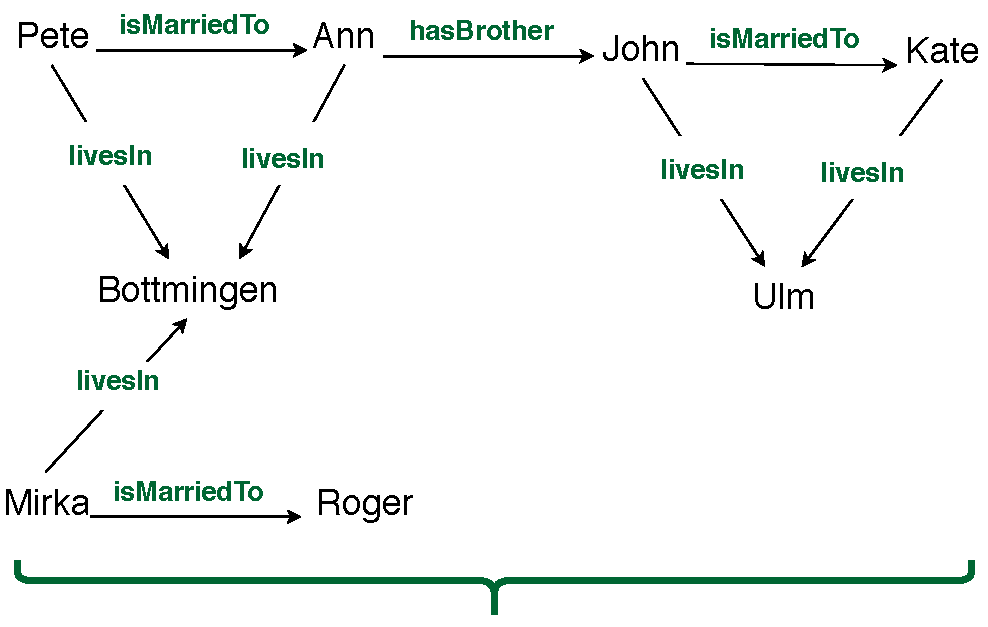
\includegraphics[width=0.8\textwidth]{hr_learn}
\huge{?}
\end{center}
\end{frame}


\begin{frame}\frametitle{\alt<2>{Inductive Learning from Interpretations}{Declarative Programming}}
\alt<2>{
 \begin{picture}(0.5,0.5)
 \put(20,-135){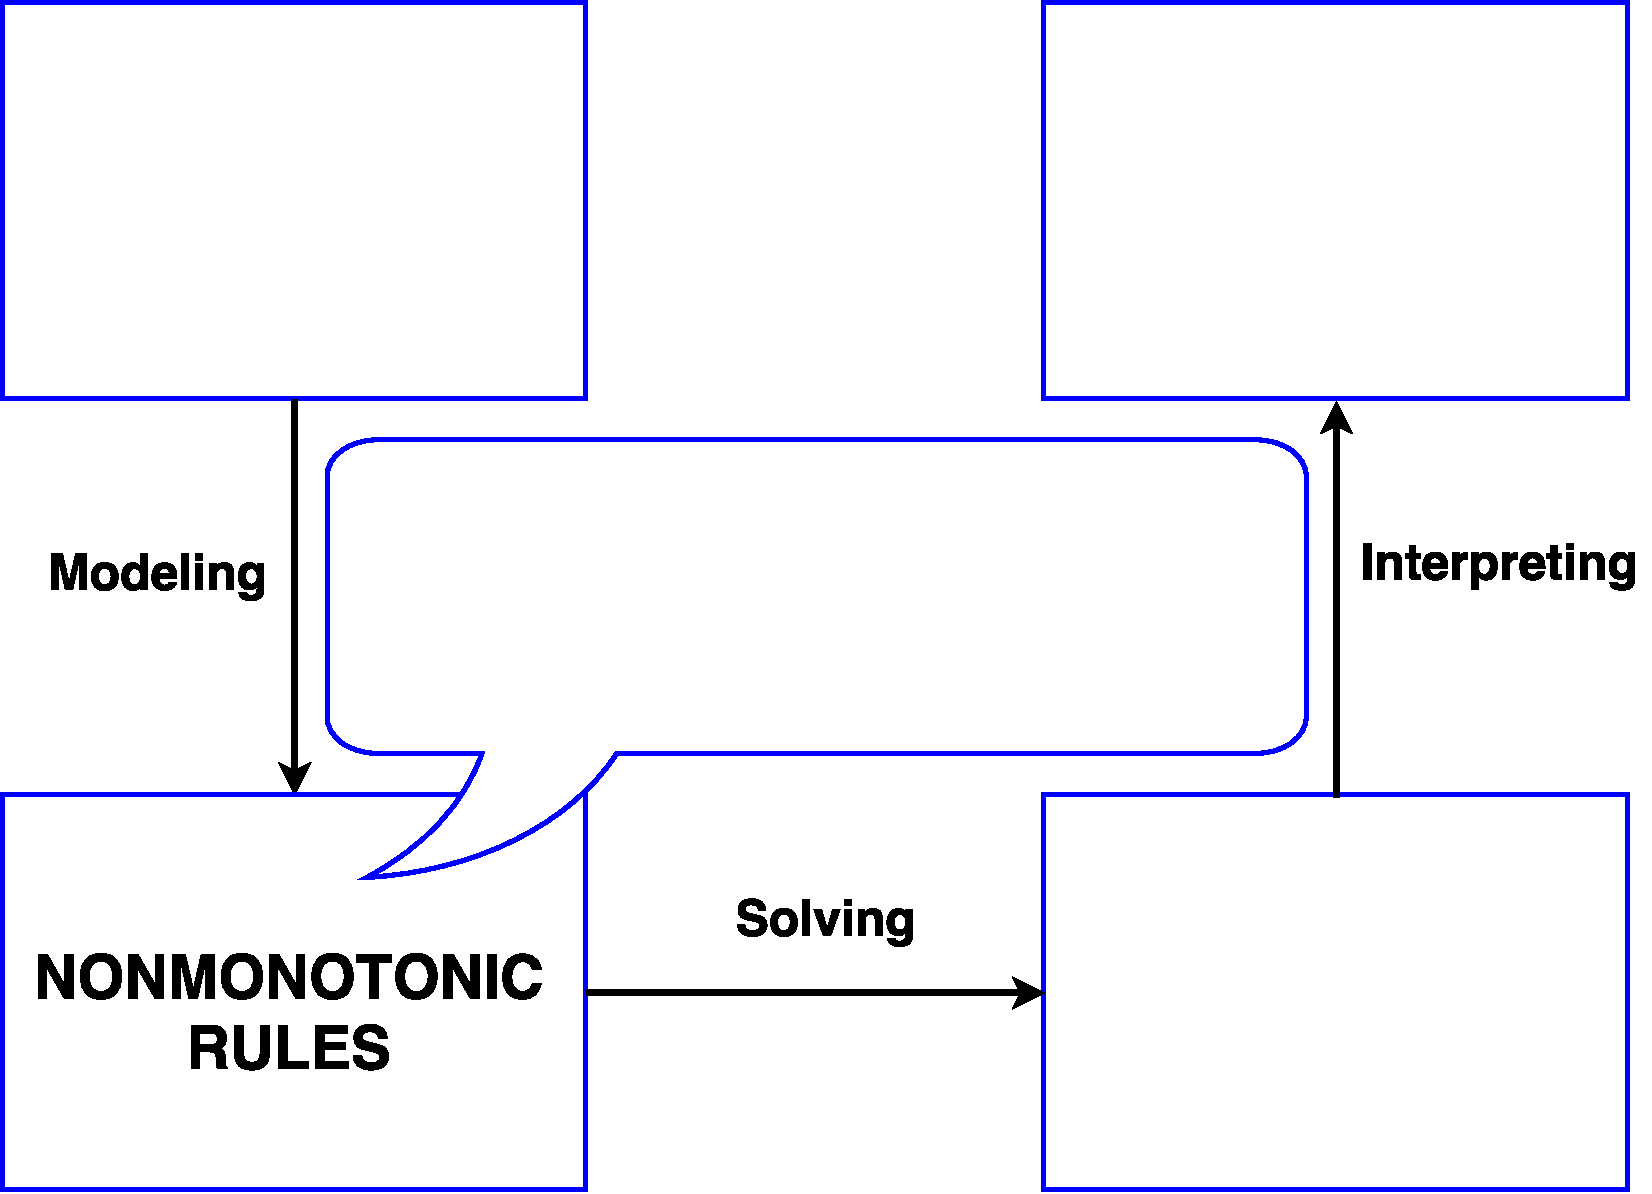
\includegraphics[width=0.9\textwidth]{asp_2}}
 \end{picture}
\put(36,65){\text{\small{Graph 3-colorability}}}

\begin{picture}(0.5,0.5)
\put(23,115){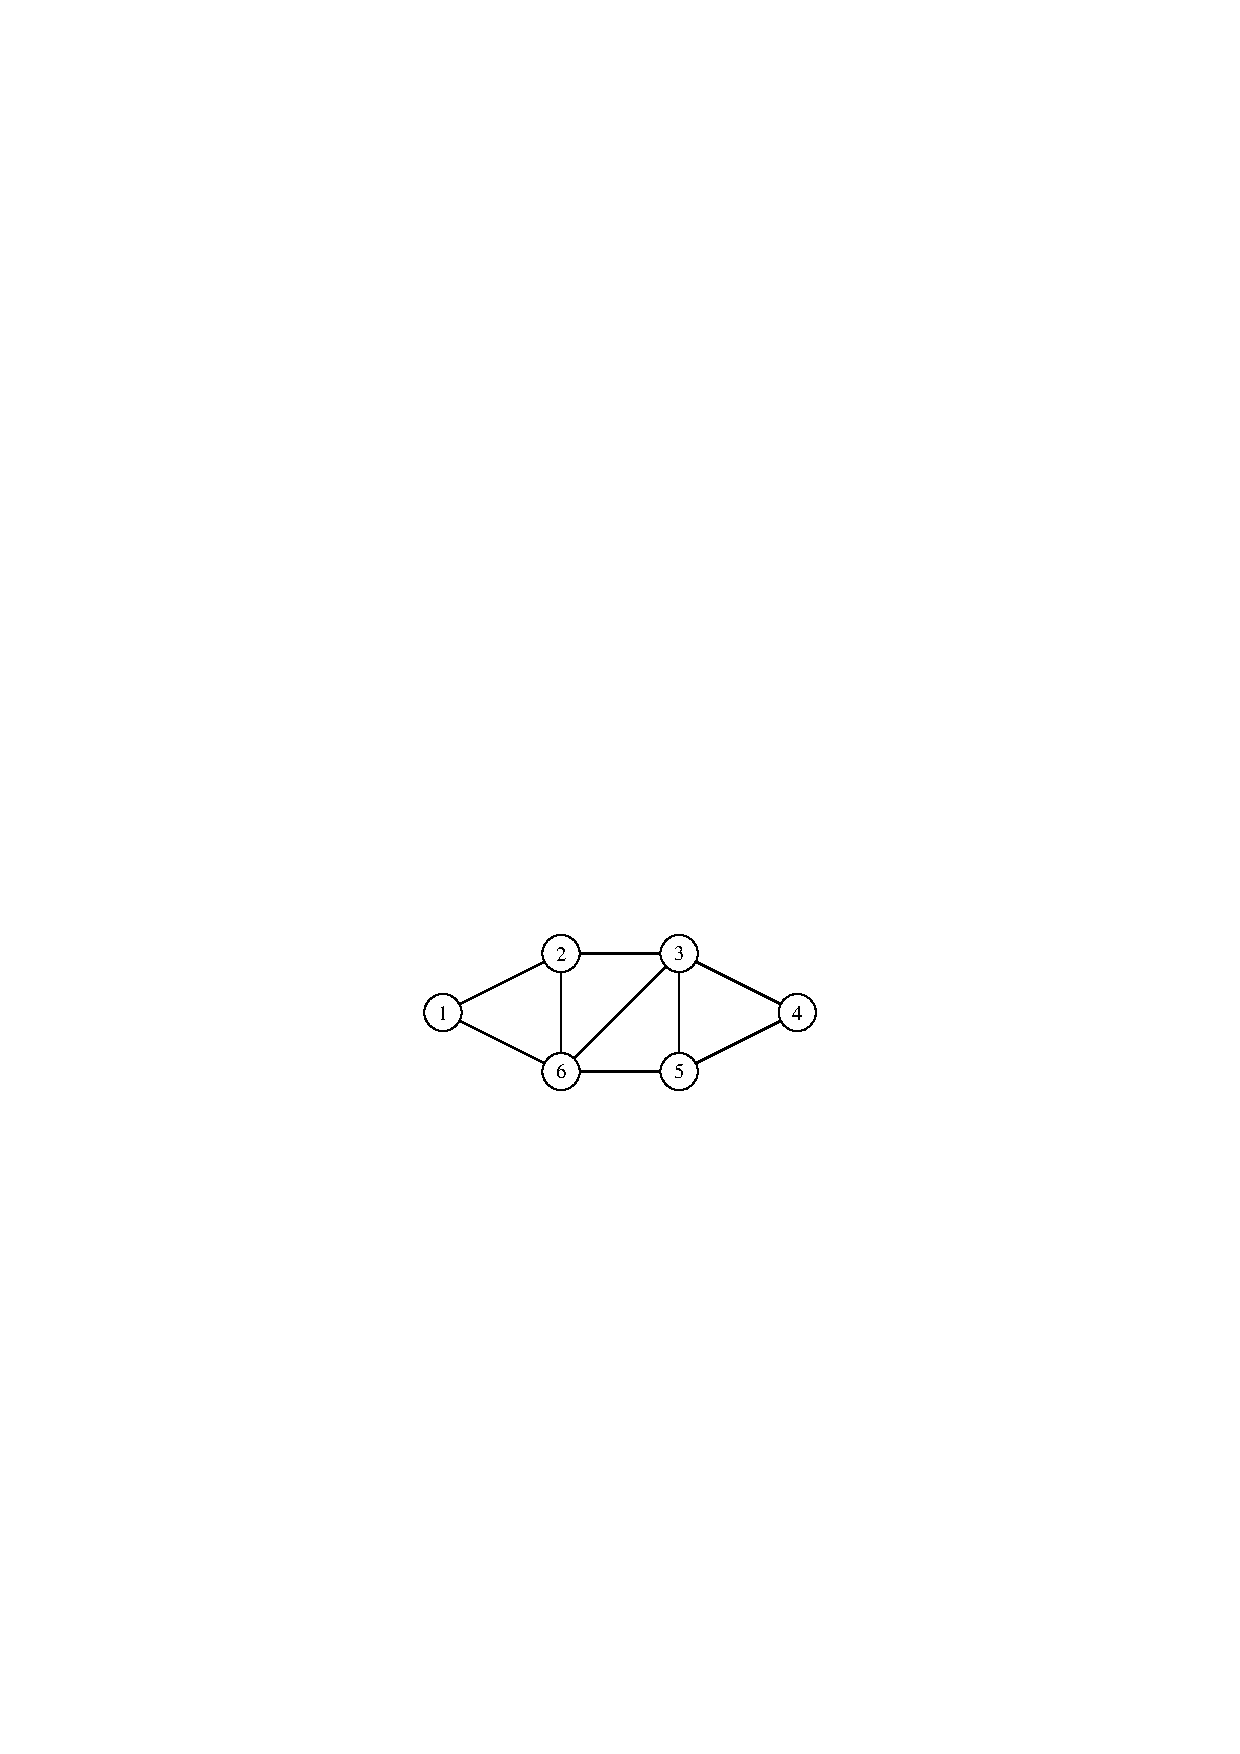
\includegraphics[width=0.32\textwidth]{graph}}
\end{picture}
\begin{picture}(0.5,0.5)
\put(208,115){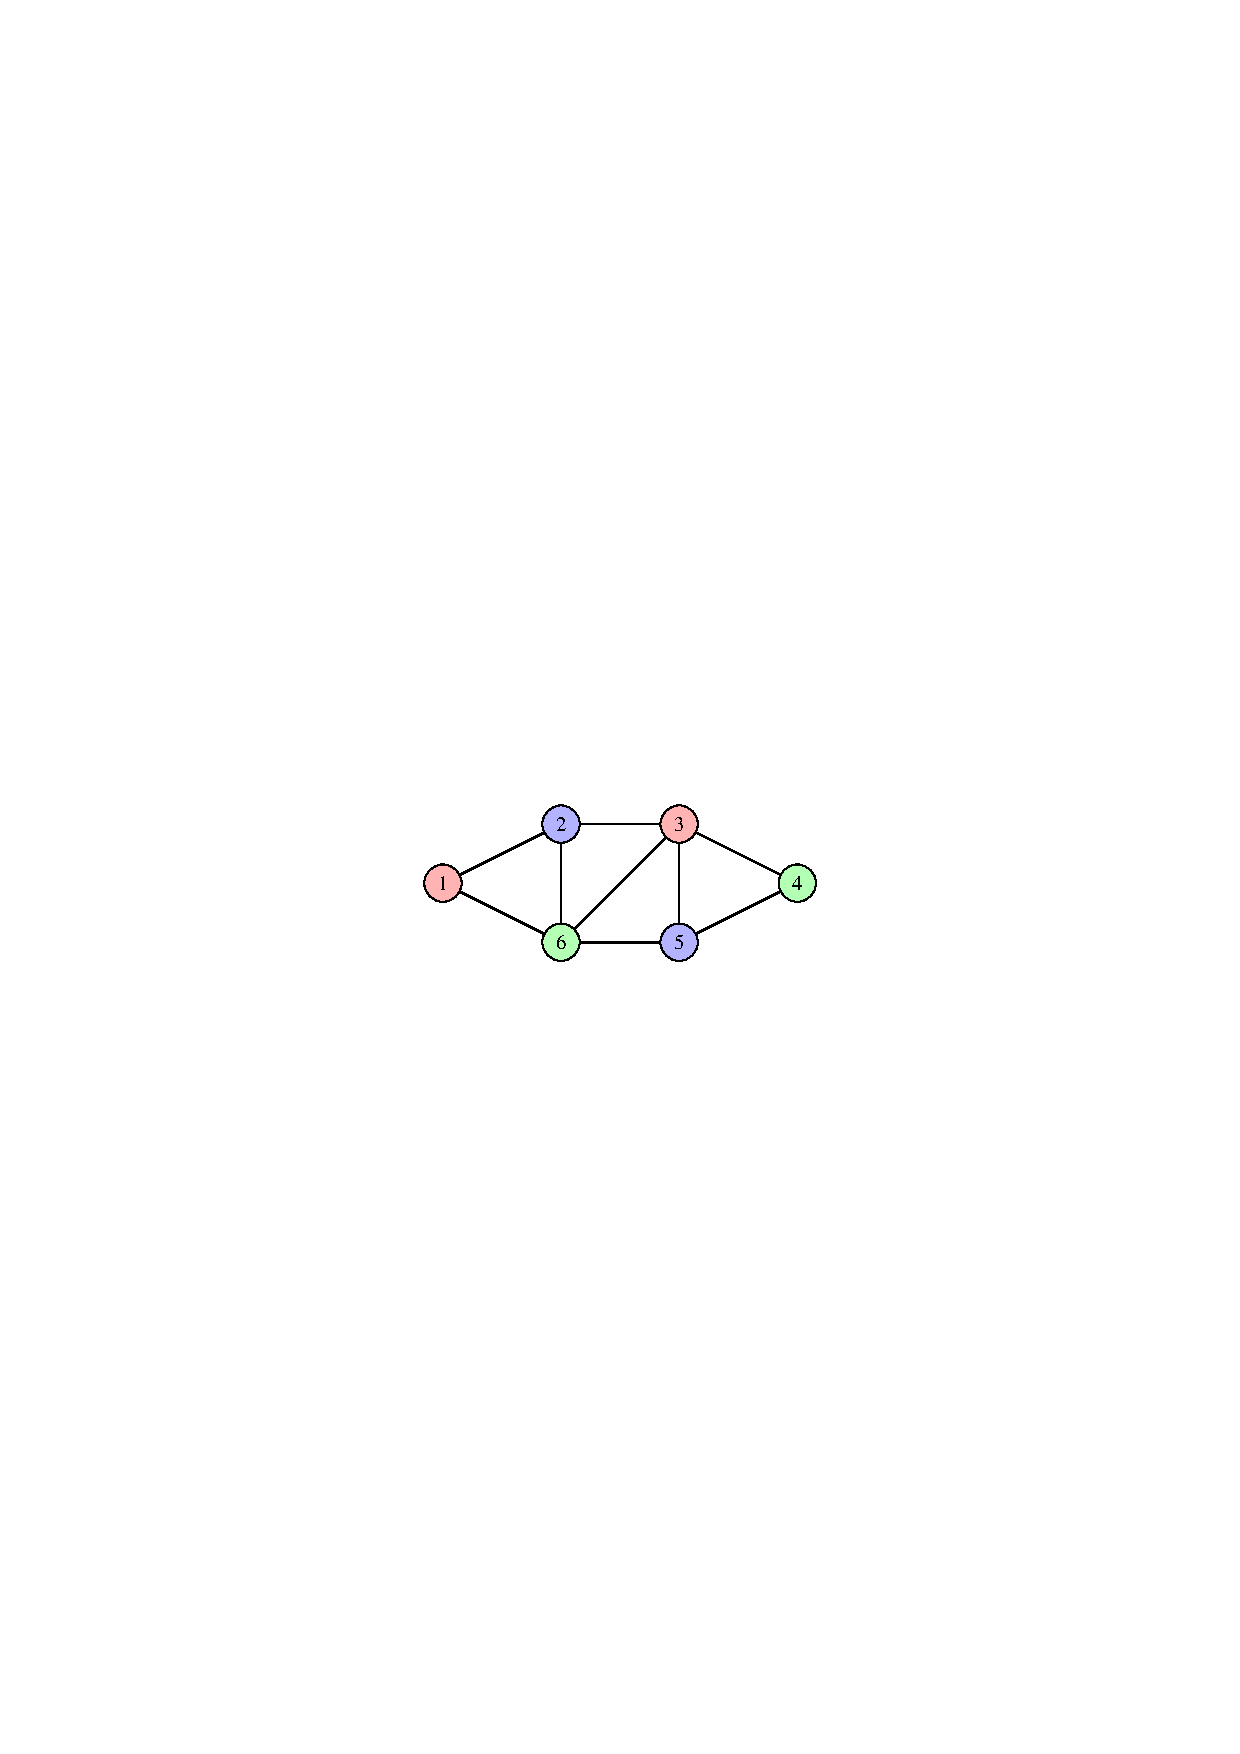
\includegraphics[width=0.32\textwidth]{graph_col}}
\end{picture}
\put(85,70){$
\tiny{
\begin{array}{@{\,}l@{~\,}}
\mi{node(1\dotsc 6)};\;\;\;\;\mi{edge(1,2)};\;\;\;\; \dotsc\\[0.35ex]
\mi{col(V,red)}\leftarrow \naf\;\mi{col(V,blue)}, \naf\;\mi{col(V,green)},\mi{node(V)};\\[0.35ex]
\mi{col(V,green)}\leftarrow \naf\;\mi{col(V,blue)},\naf\;\mi{col(V,red)},\mi{node(V)};\\[0.35ex]
\mi{col(V,blue)}\leftarrow \naf\;\mi{col(V,green)},\naf\;\mi{col(V,red)},\mi{node(V)};\\[0.35ex]
\bot\leftarrow \mi{col(V,C)},\mi{col(V,C')},C \neq C';\\[0.35ex]
\bot \leftarrow \mi{col(V,C)},\mi{col(V',C)}, \mi{edge(V,V')}\\[0.35ex]
\end{array}}
$}
 \put(215,0){\tiny{$\begin{array}{@{\,}l@{~\,}}
\mi{node(1\dotsc 6)};\;\;\;\;\mi{edge(1,2)};\dotsc\\ \mi{col(1, red),col(2,blue)},\\ \mi{col(3,red),col(4,green)},\\ \mi{col(6,green),col(5,blue)}\end{array}$}}
}{
\begin{picture}(0.5,0.5)
\put(20,-120){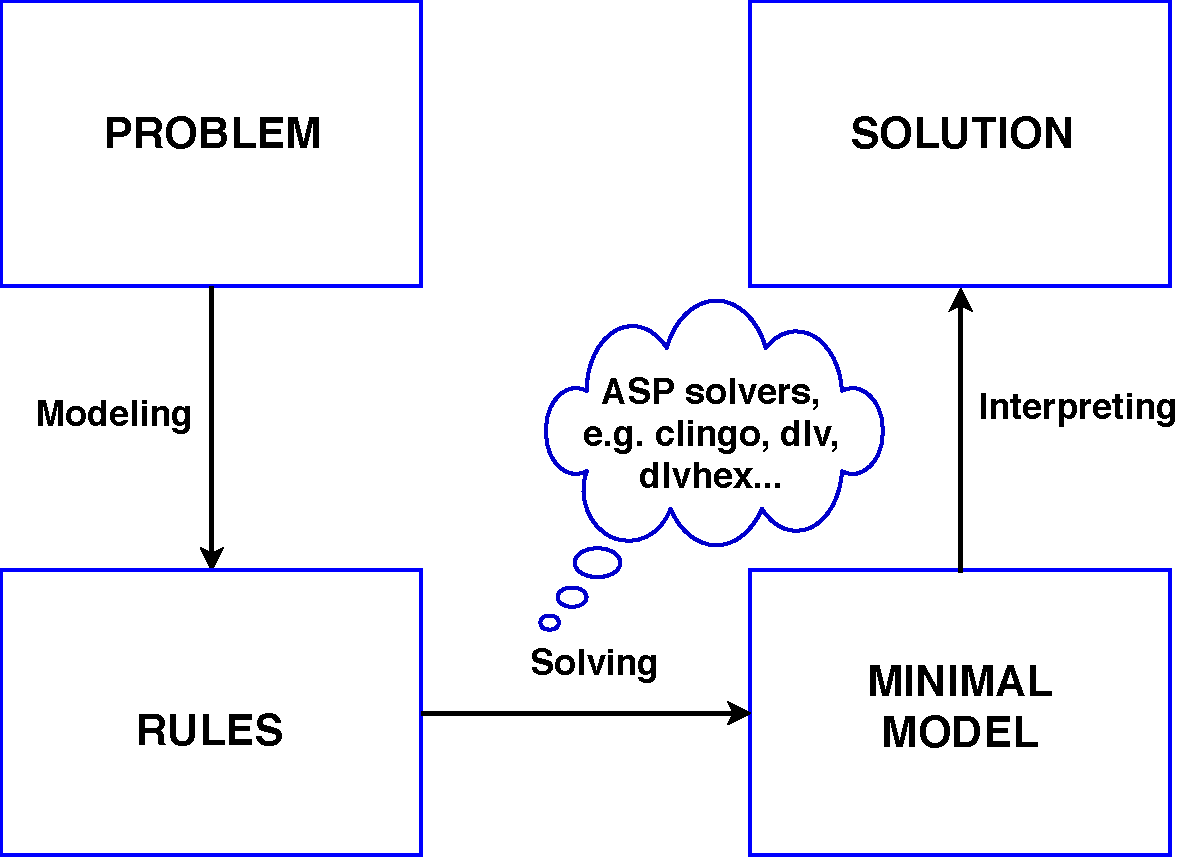
\includegraphics[width=0.86\textwidth]{asp_1}}
\end{picture}
}
\end{frame}


\begin{frame}\frametitle{Rule Induction}
%\alt<2>{\begin{picture}(0.5,0.5)
%\put(20,-190){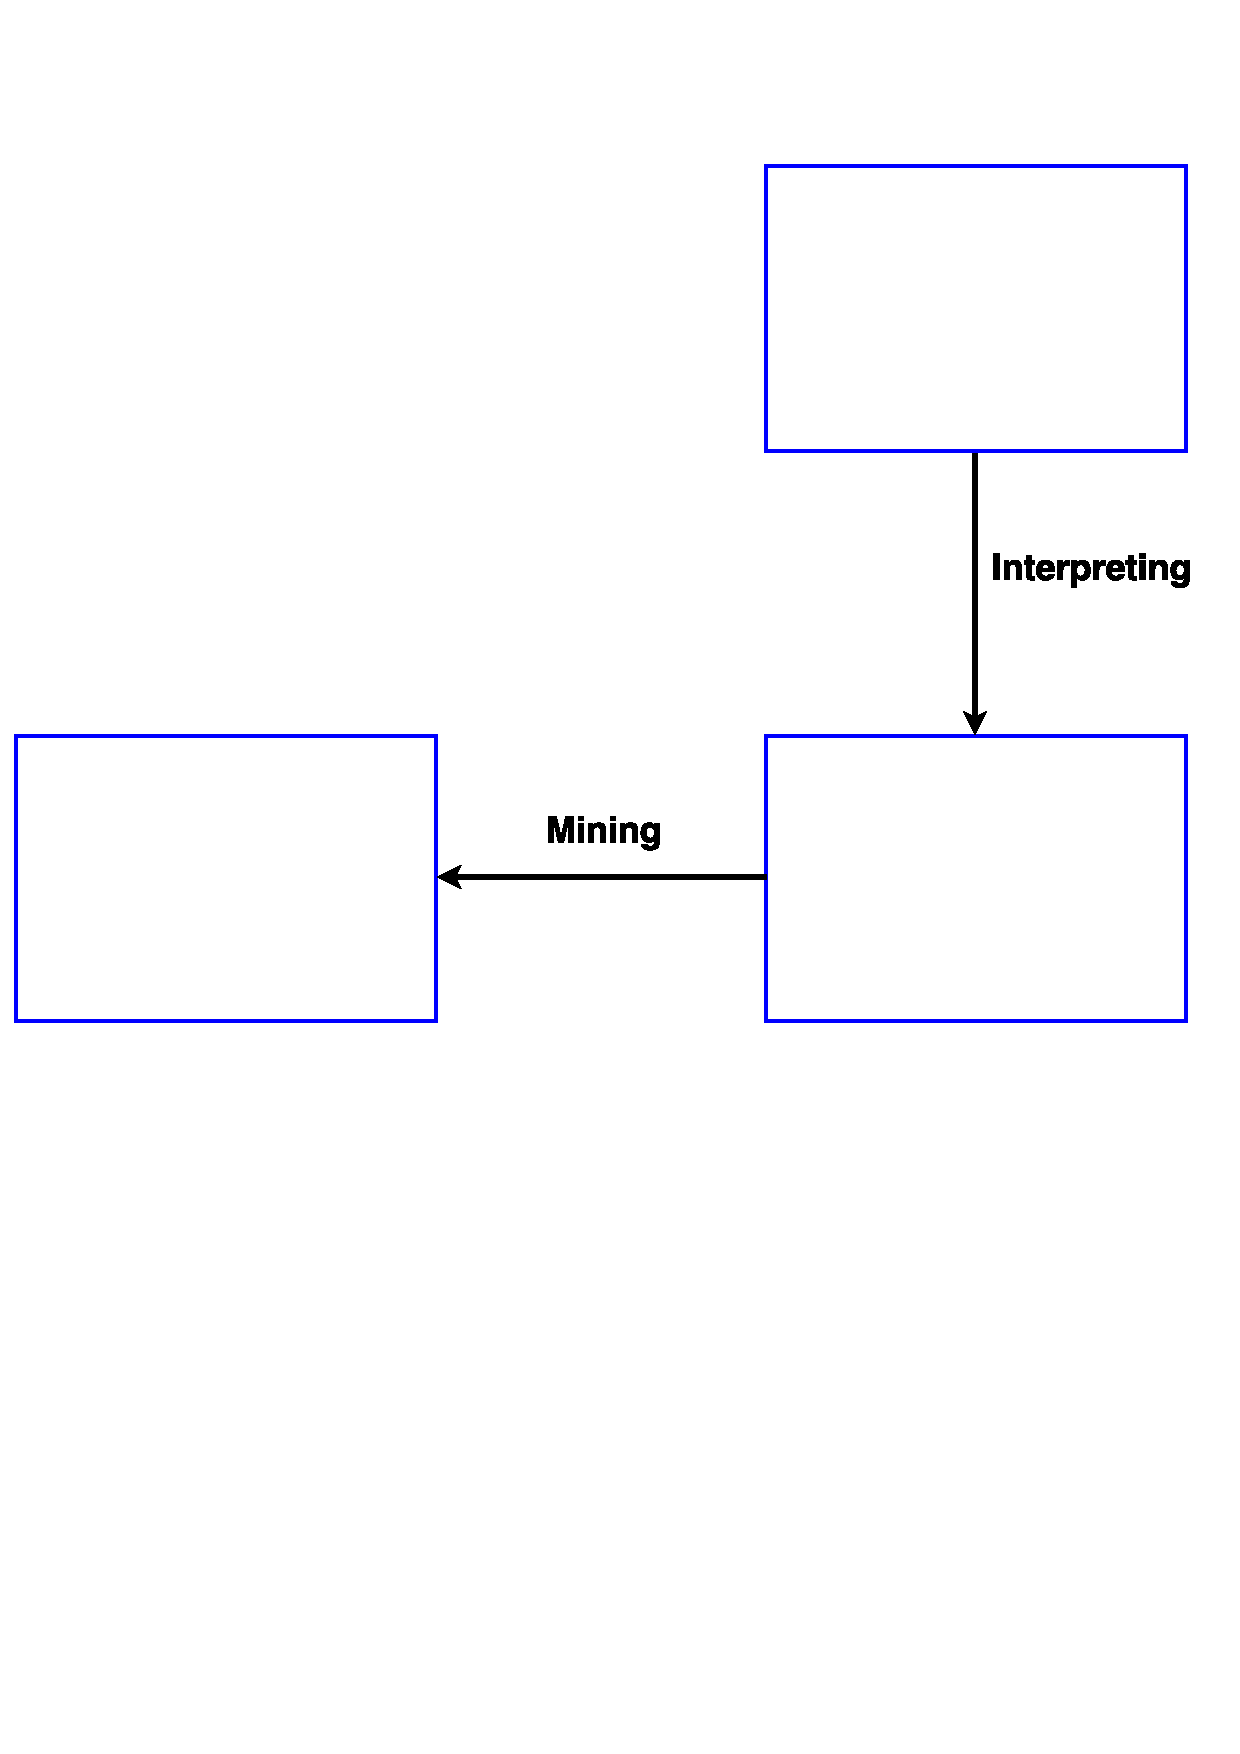
\includegraphics[width=0.86\textwidth]{asp_4}}
%\end{picture}

%\begin{picture}(0.5,0.5)
%\put(209,-35){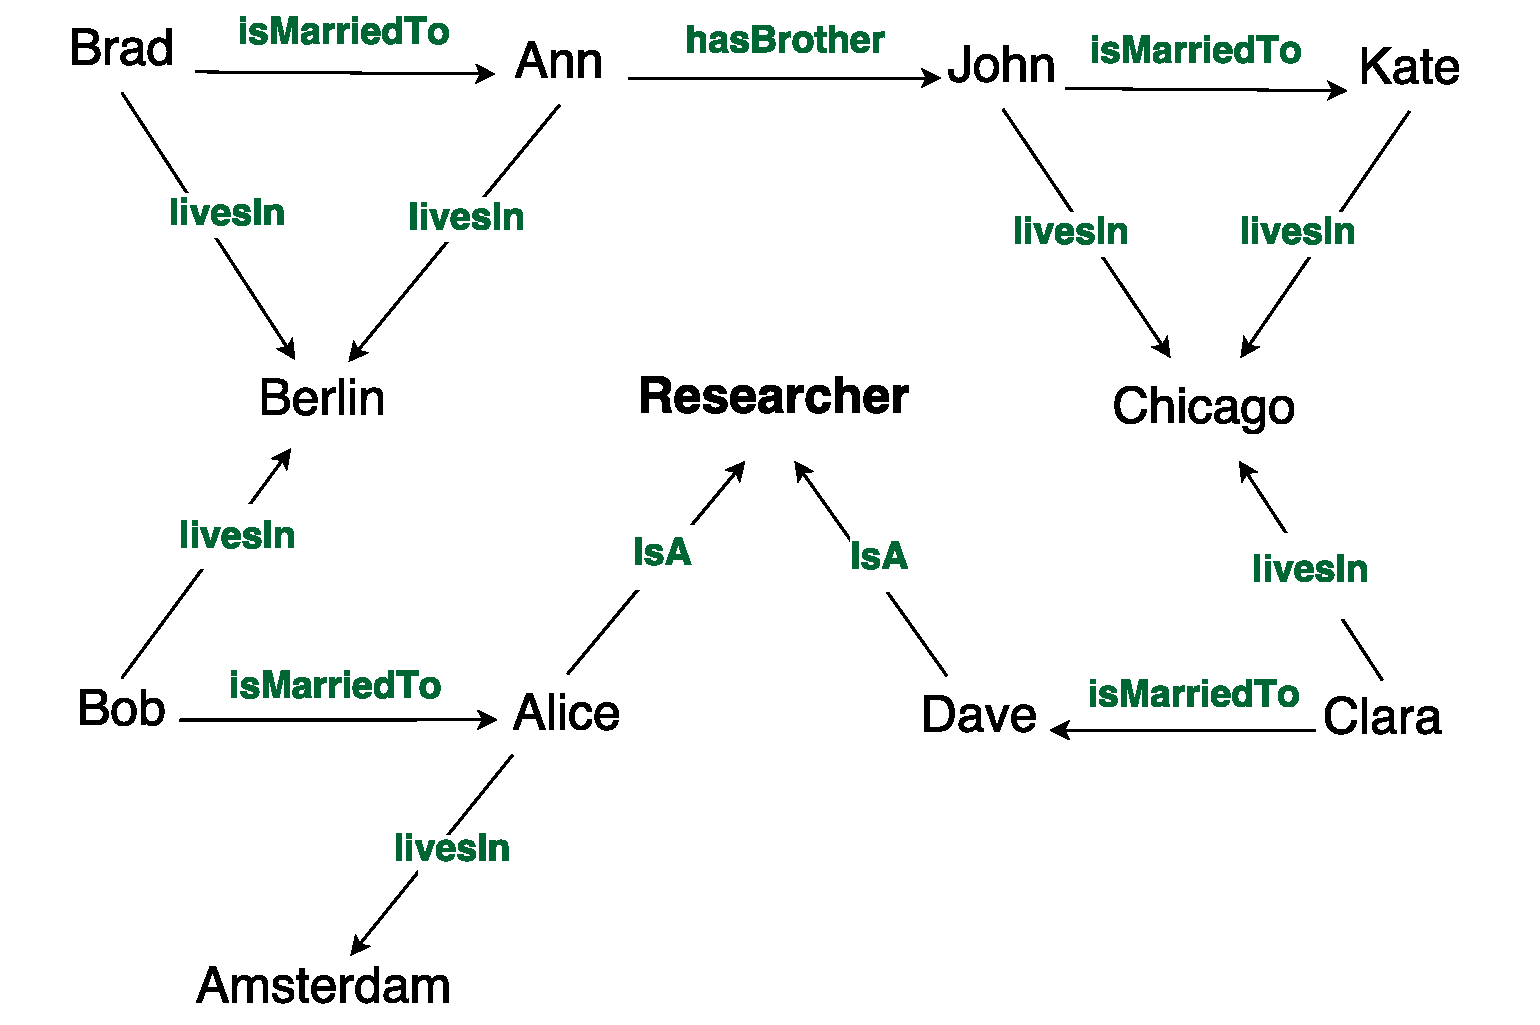
\includegraphics[width=0.258\textwidth]{kg0}}
%\end{picture}
% \put(26,-138){\gr{\tiny{$\begin{array}{@{\,}l@{~\,}}
% \mi{livesIn(Y,Z)}\leftarrow \mi{isMarried(X,Y)}, \\
% \phantom{\mi{livesIn(Y,Z)}\leftarrow} \mi{livesIn(X,Y)}, \\ \phantom{\mi{livesIn(Y,Z)}\leftarrow}\naf\ \mi{researcher(Y)}\end{array}
% $}}}
%  \put(209,-138){\gr{\tiny{$\begin{array}{@{\,}l@{~\,}}
% \mi{\gr{isMarriedTo}(brad,ann)};\\ \mi{\gr{isMarriedTo}(john,kate)};\\ \mi{\gr{isMarriedTo}(bob,alice)};\\ \mi{\gr{isMarriedTo}(clara, dave)}; \\ \mi{\gr{livesIn}(brad,berlin};\\ \dotsc\\ \mi{researcher(alice)};\\ \mi{researcher(dave)}\end{array}$}}}
% }{
  \begin{picture}(0.5,0.5)
\put(20,-120){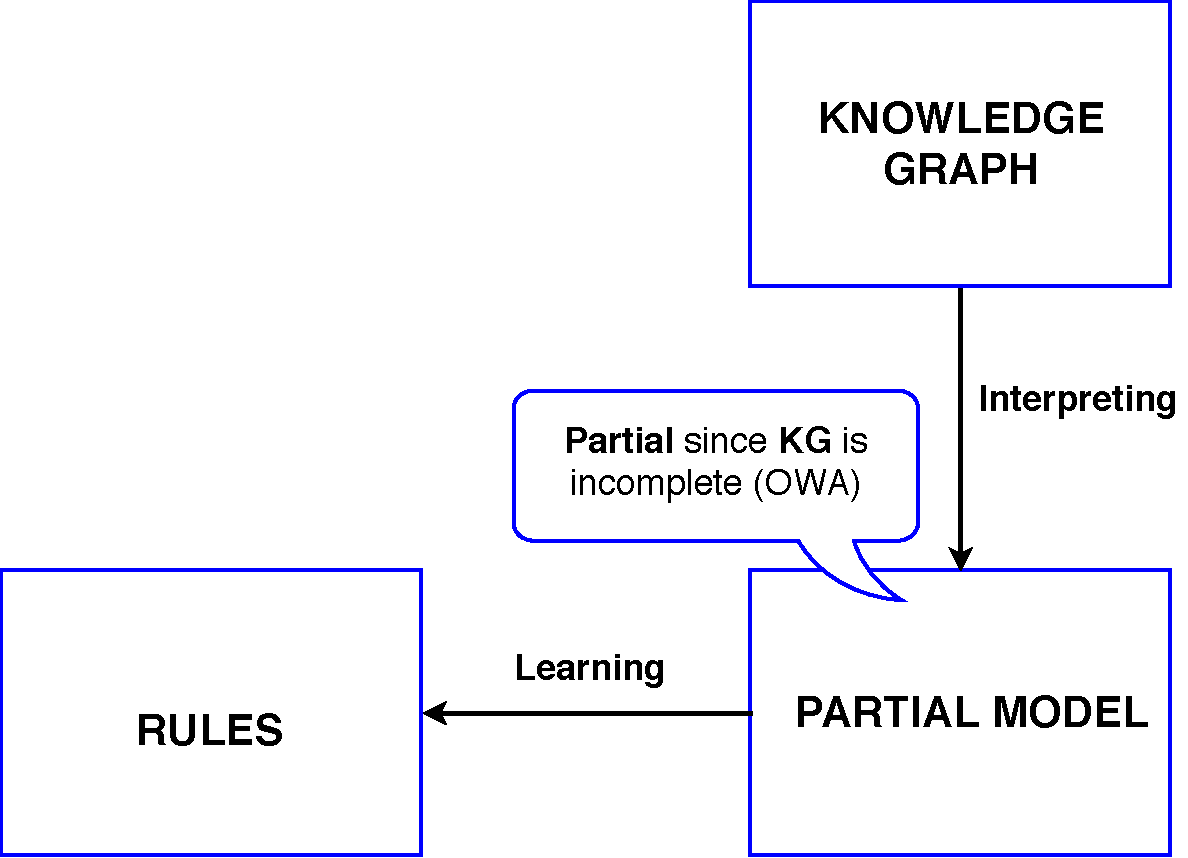
\includegraphics[width=0.86\textwidth]{asp_3}}
\end{picture}
%}
\end{frame}

\subsection{KG Challenges}
\begin{frame}\frametitle{Challenges of Rule Induction from KGs}
\begin{itemize}
\item[] \textbf{\bl{Open World Assumption}}: Negative examples are unavaible
\medskip
\pause 

\emph{Maybe Albert Einstein was a ballet dancer?}
\end{itemize}
\bigskip
\begin{center}
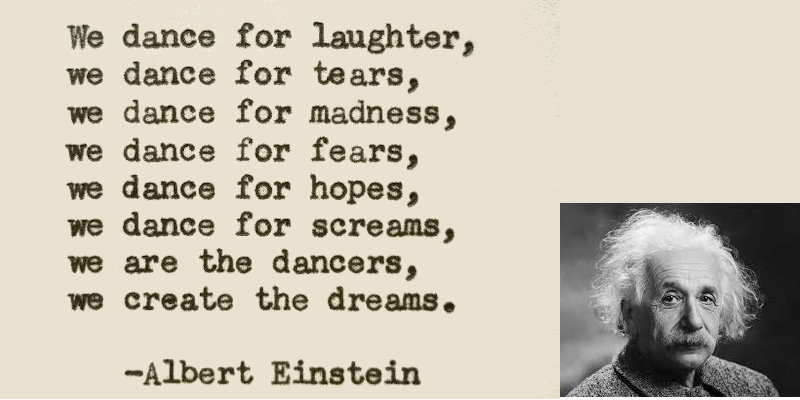
\includegraphics[width=0.86\textwidth]{owa_einstein}
\end{center}
\end{frame}

\begin{frame}\frametitle{Challenges of Rule Induction from KGs} 
\begin{itemize}
\item[] \textbf{\bl{Data bias}}: Only interesting facts are mentioned in text
\medskip
\pause 

\emph{E.g., as wikipedia stores mostly famous people, one can induce wrong assumptions that all scientists are Nobel prize winners or all inhabitants of ancient Egypt are pharaons..}
\end{itemize}
\bigskip
\begin{center}
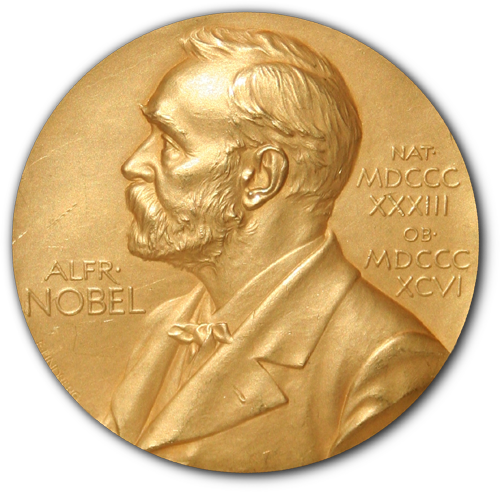
\includegraphics[width=0.3\textwidth]{noble}  \;\;\;
\includegraphics[width=0.2\textwidth]{pharaon} 
\end{center}
\end{frame}

\begin{frame}\frametitle{Challenges of Rule Induction from KGs}
\begin{itemize}
\item[] \textbf{\bl{Huge size}}: Modern KGs contain billions of facts \\
\end{itemize}
\bigskip
\begin{center}
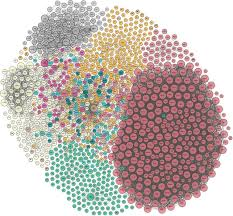
\includegraphics[width=0.5\textwidth]{hugekg}
\end{center}
\end{frame}

\begin{frame}\frametitle{Challenges of Rule Induction from KGs}
\begin{itemize}
\item \textbf{\bl{World knowledge is complex}}, none of its ``models'' is perfect
\end{itemize}
\bigskip
\begin{center}
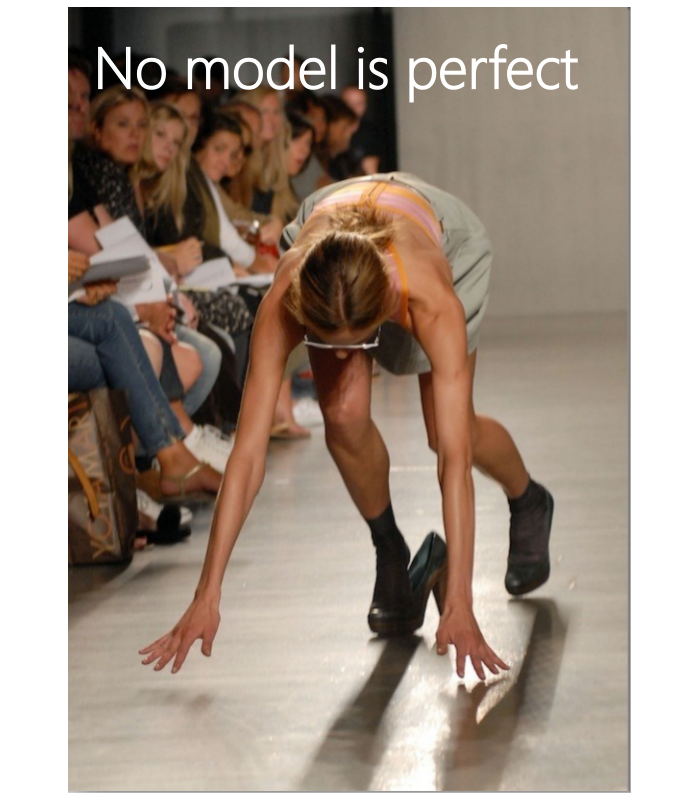
\includegraphics[width=0.5\textwidth]{noperfectmodel}
\end{center}

\end{frame}

\subsection{Association Rules}
\begin{frame}\frametitle{Exploratory Data Analysis}
\smallskip

 \begin{beamerboxesrounded}[upper=uppercolblue,lower=lowercolblue,shadow=true]{\textbf{\bl{Question:}}}
How can we still learn interesting rules from KGs, which do not perfectly fit the data, but still reflect interesting correlations and can predict sufficiently many correct facts?
\end{beamerboxesrounded}
\bigskip

 \begin{beamerboxesrounded}[upper=uppercolblue,lower=lowercolblue,shadow=true]{\textbf{\bl{Answer:}}} Relational association rule mining!
\end{beamerboxesrounded}

\begin{center}
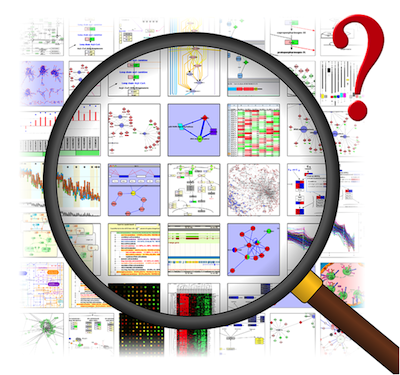
\includegraphics[width=0.3\textwidth]{eda}
\end{center}
\end{frame}


\begin{frame}\frametitle{Association Rules}

\begin{itemize}
\item Which products are often bought together?
\item 

\end{itemize}
\end{frame}


\begin{frame}\frametitle{How to Apply Ideas to Relational Data?}
\end{frame}

\begin{frame}\frametitle{Propositionalization}
\end{frame}

\subsection{Relational Association Rules}

\begin{frame}\frametitle{Relational Association Rule Mining}
\end{frame}

\begin{frame}\frametitle{WARMER}
\end{frame}

\begin{frame}\frametitle{AMIE}
\end{frame}

\begin{frame}\frametitle{RDF2Rules}
\end{frame}

\begin{frame}\frametitle{Ontology Path Finding}
\end{frame}




\section{Exception-awareness}
\begin{frame}\frametitle{\alt<4>{Nonmonotonic Rule Mining}{Horn Rule Mining}}
\smallskip

\uncover<2->{\alt<4->{\bl{Nonmonotonic rule mining} from KGs: \alert{OWA} is a challenge!}{\bl{Horn rule} mining for KG \bl{completion} \cite{amie} } }
 \bigskip
 \bigskip
 \bigskip
 \bigskip
 \bigskip
 \bigskip
 \bigskip
 \bigskip
 \bigskip
 \bigskip
 \bigskip
 \bigskip
 \bigskip
 \bigskip
 \bigskip
 \bigskip

\alt<4->{\begin{picture}(0.5,0.5)\put(43,-33){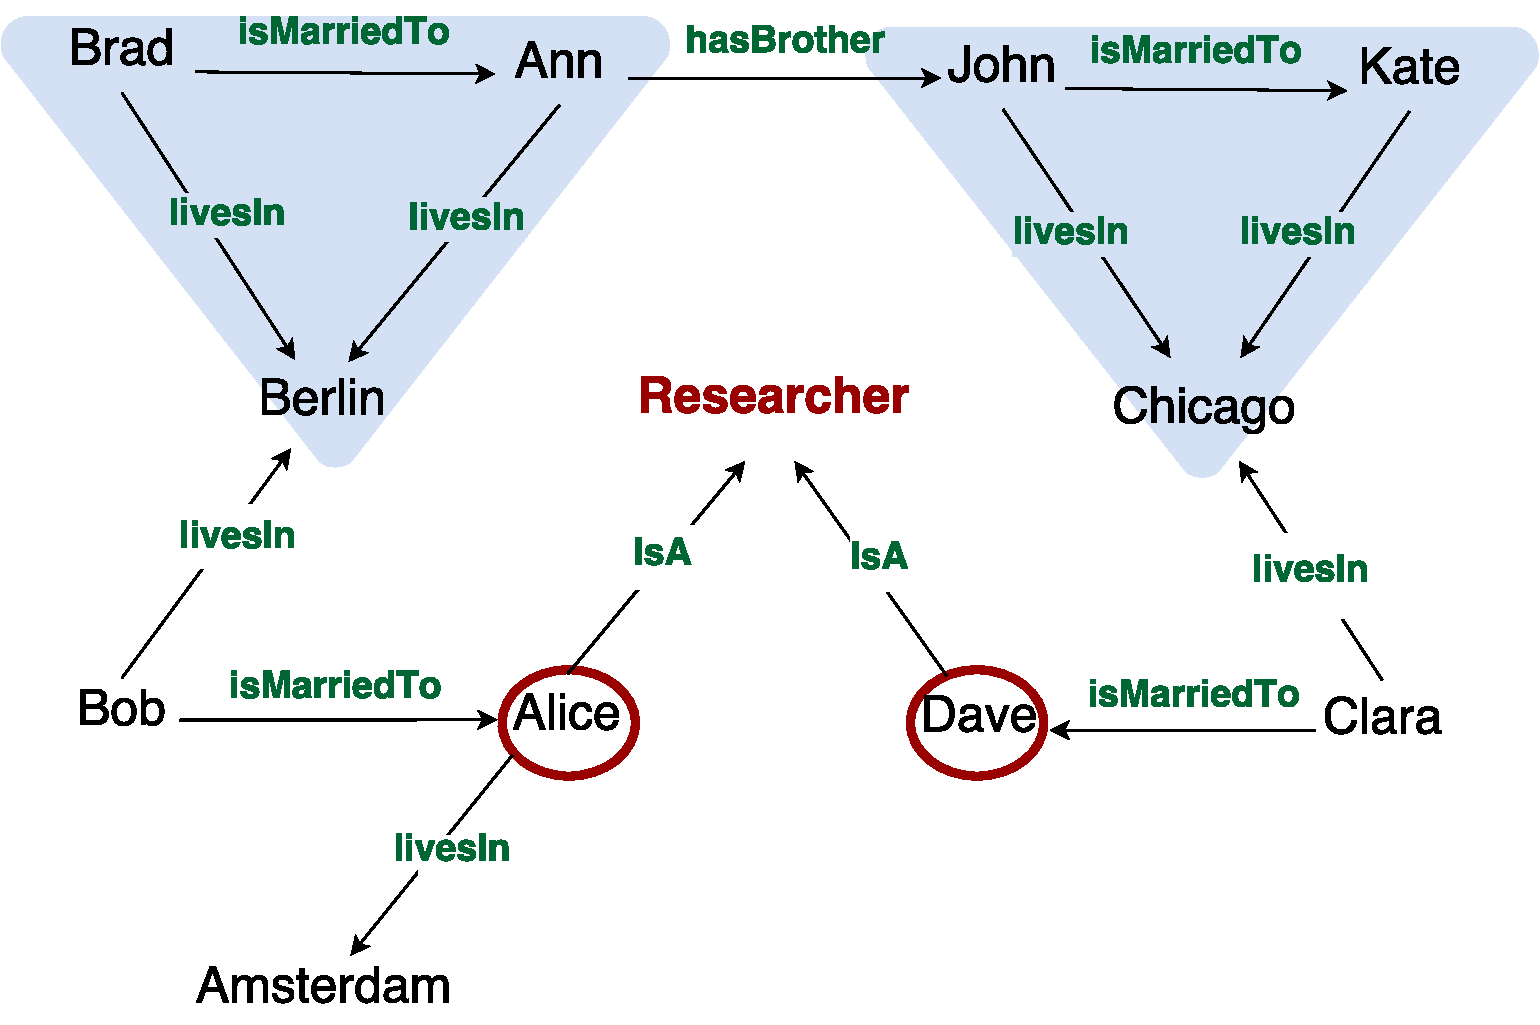
\includegraphics[width=0.75\textwidth]{kg3}}\end{picture}}{
\alt<3->{
\begin{picture}(0.5,0.5)\put(43,-33){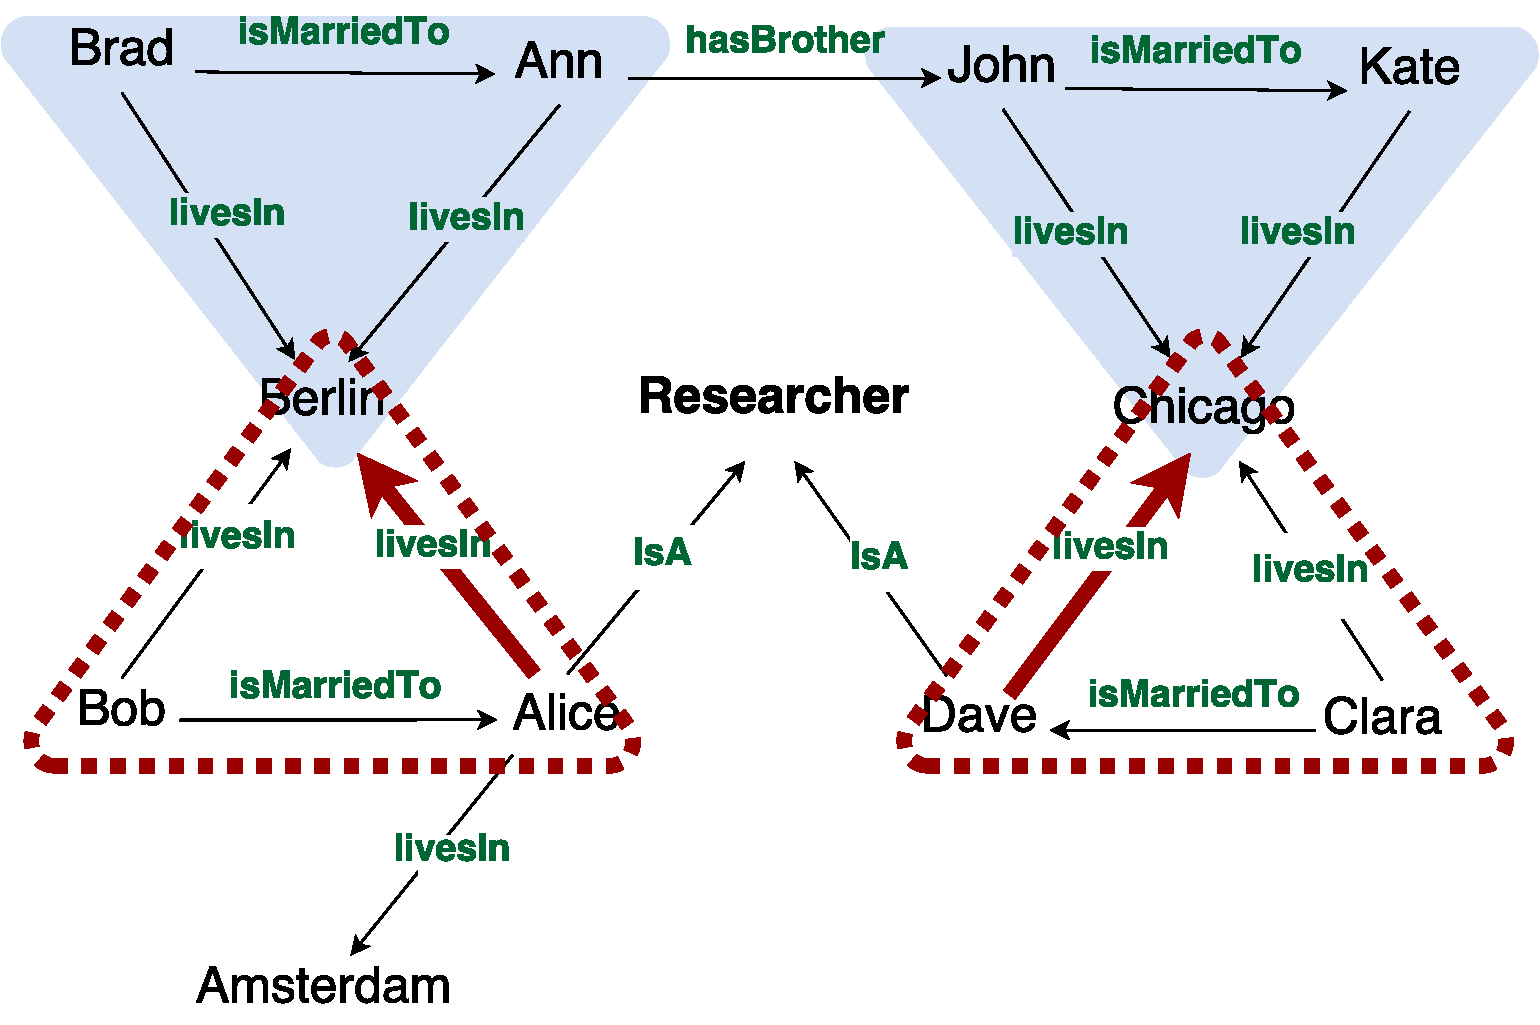
\includegraphics[width=0.75\textwidth]{kg2}}\end{picture}
}{\alt<2->{\begin{picture}(0.5,0.5)\put(43,-33){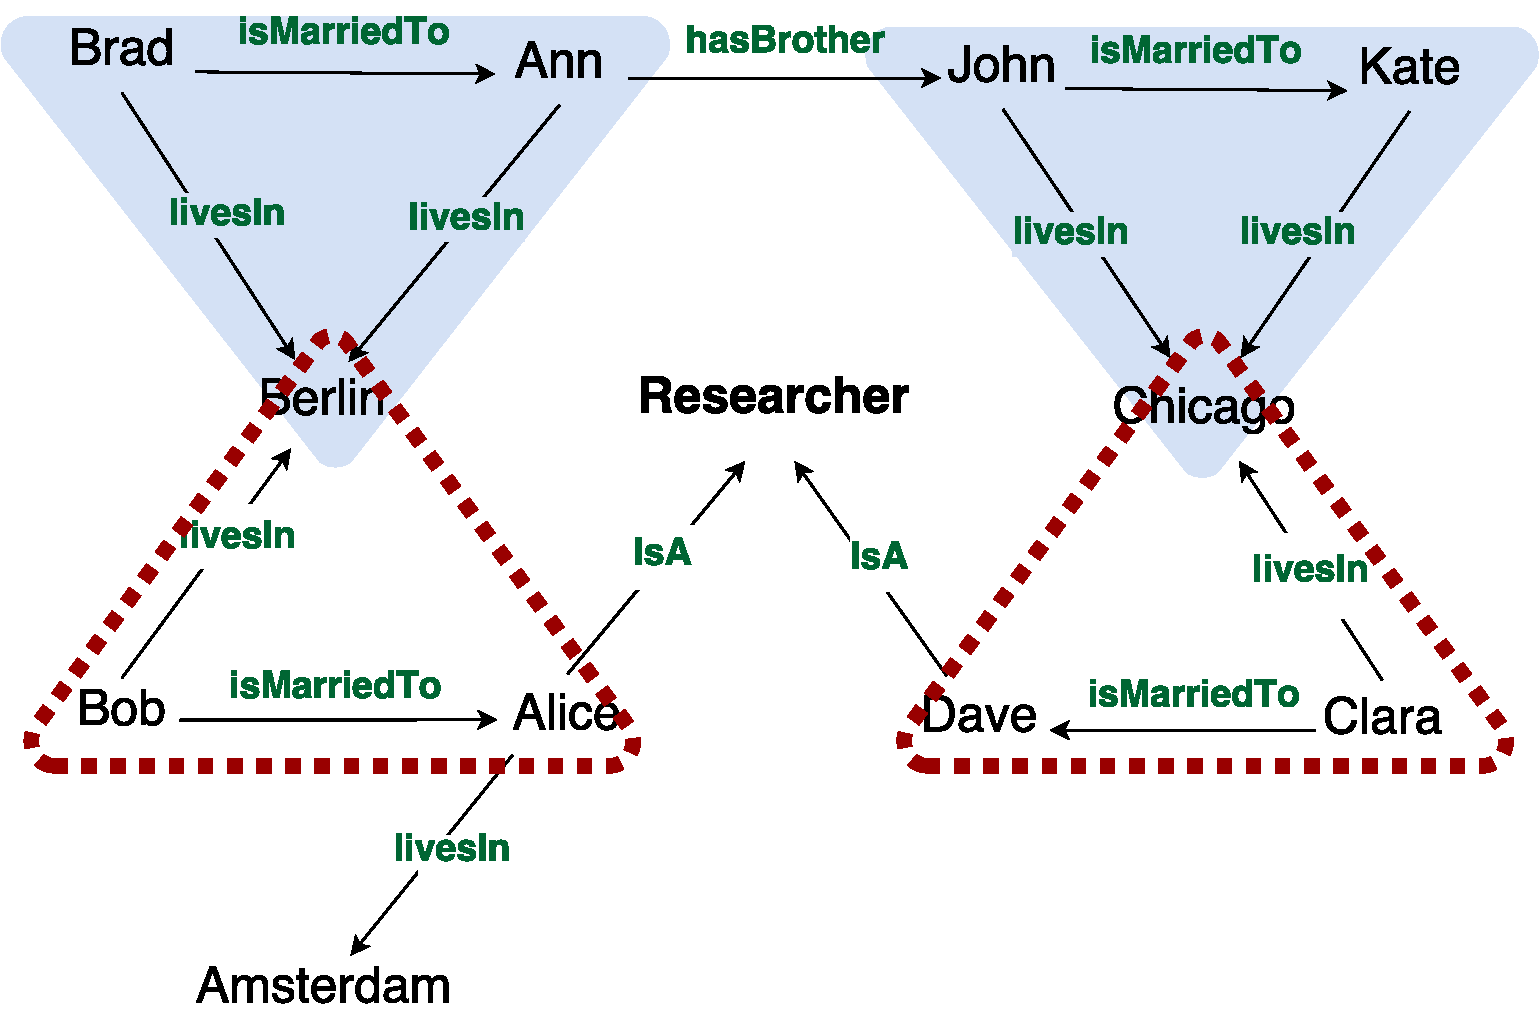
\includegraphics[width=0.75\textwidth]{kg1}}\end{picture}}{\begin{picture}(0.5,0.5)\put(43,-33){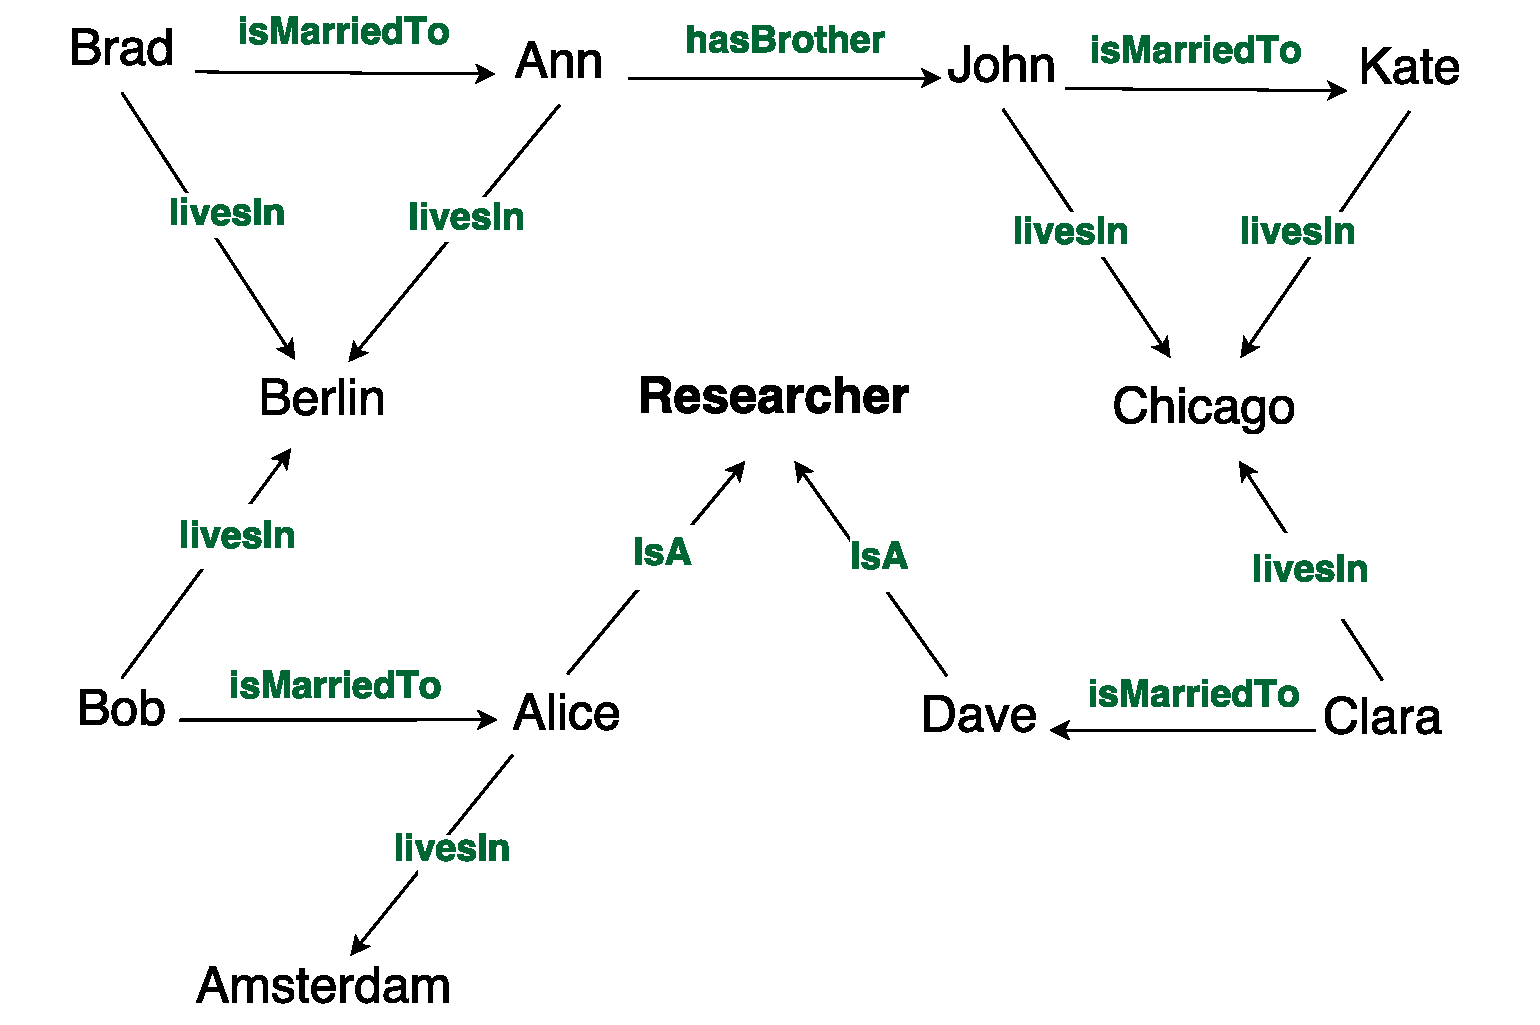
\includegraphics[width=0.75\textwidth]{kg0}}\end{picture}}}}
\begin{center}
\visible<2->{\rightline{\gr{$\mi{conf(r)}=\dfrac{|\myfilledtriangle{lightblue}|}{|\myfilledtriangle{lightblue}|+|\mytriangle{darkred}{white}|}=$\alt<4>{$1$}{$\dfrac{2}{4}$}}}}
\bigskip
\bigskip

\uncover<2->{\normalsize{\alt<4>{\textcolor{darkgreen}{$r:\;\mi{livesIn(X,Z)}\leftarrow \mi{isMarriedTo(Y,X),livesIn(Y,Z)},$}\,\alert{$\naf\ researcher(X)$}}{\textcolor{darkgreen}{$r:\;\mi{livesIn(X,Z)}\leftarrow \mi{isMarriedTo(Y,X),livesIn(Y,Z)}$}}}}
 \end{center}

\end{frame}




% \begin{frame}\frametitle{Nonmonotonic Rule Mining}
% \alt<2>{\begin{picture}(0.5,0.5)
% \put(20,-190){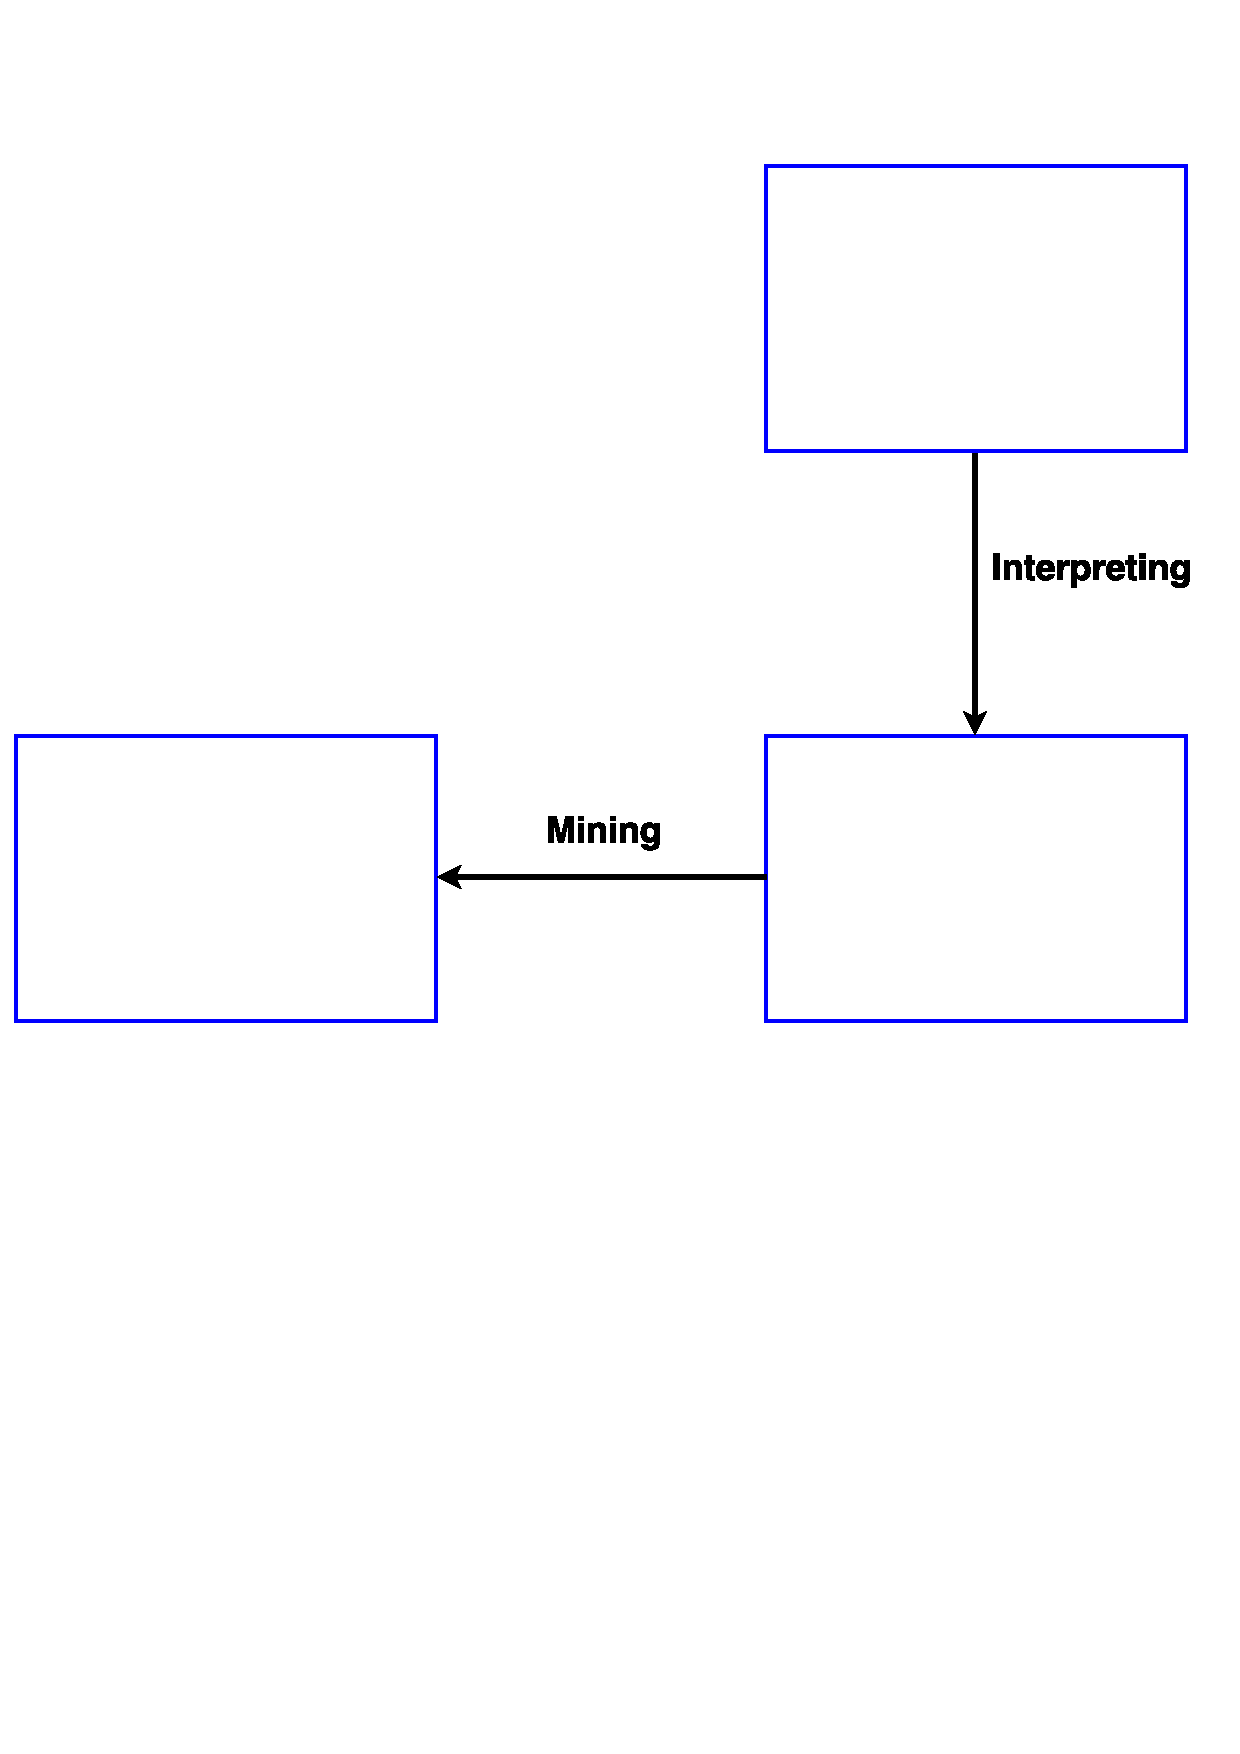
\includegraphics[width=0.86\textwidth]{asp_4}}
% \end{picture}

% \begin{picture}(0.5,0.5)
% \put(209,-35){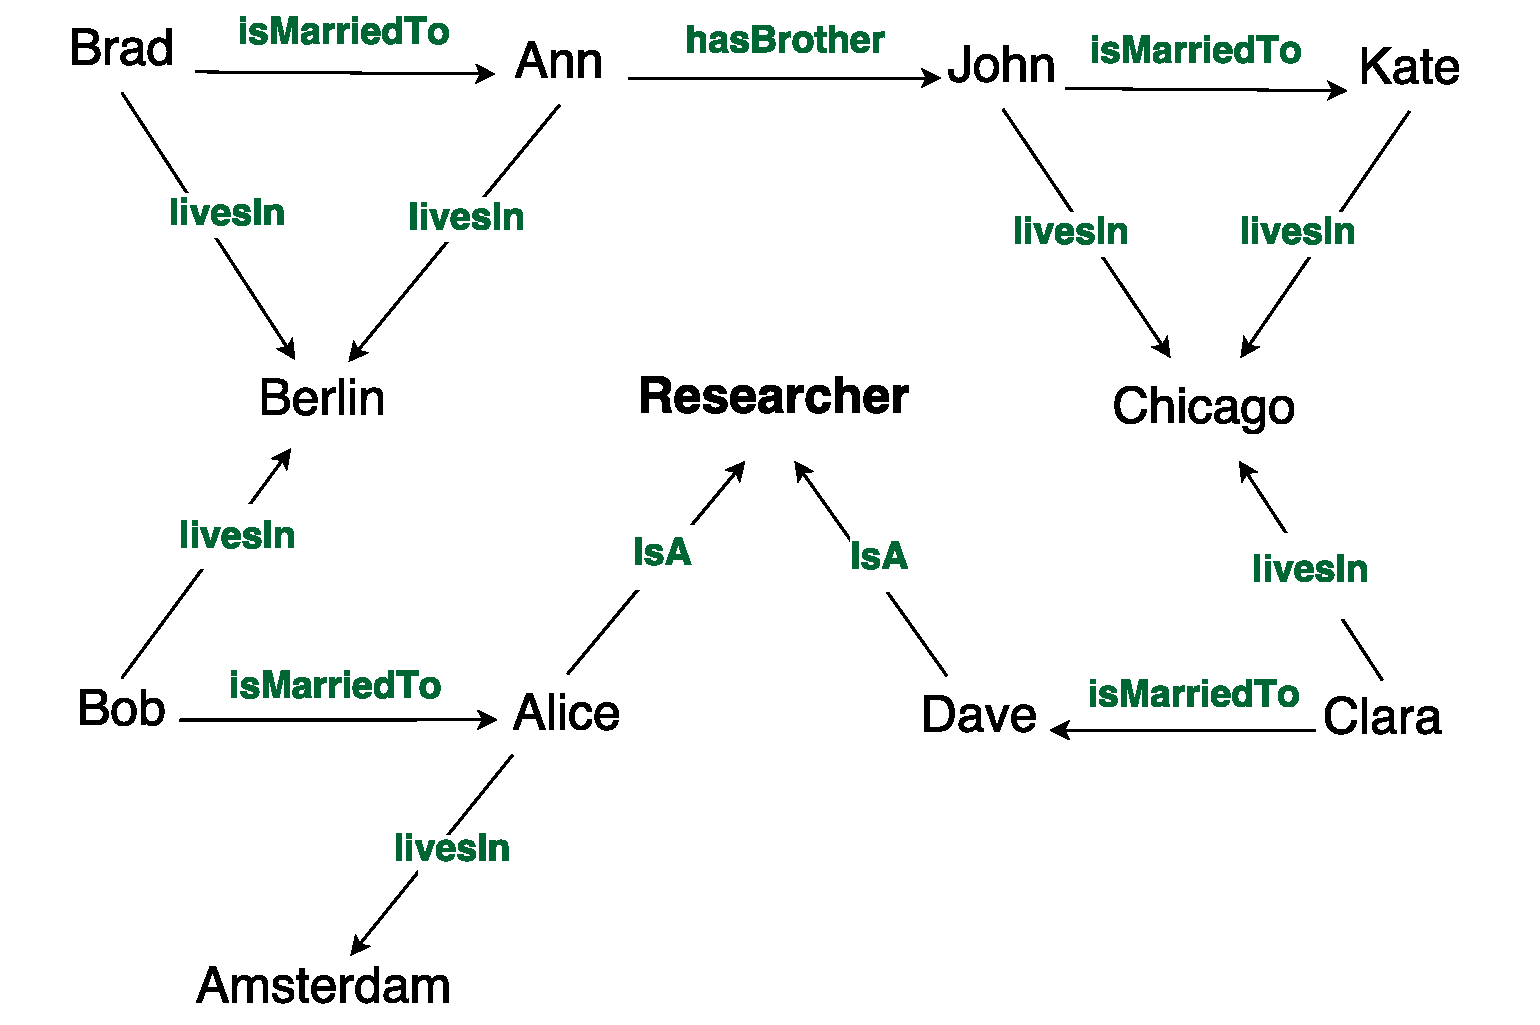
\includegraphics[width=0.258\textwidth]{kg0}}
% \end{picture}
% \put(26,-138){\gr{\tiny{$\begin{array}{@{\,}l@{~\,}}
% \mi{livesIn(Y,Z)}\leftarrow \mi{isMarried(X,Y)}, \\
% \phantom{\mi{livesIn(Y,Z)}\leftarrow} \mi{livesIn(X,Y)}, \\ \phantom{\mi{livesIn(Y,Z)}\leftarrow}\naf\ \mi{researcher(Y)}\end{array}
% $}}}
%  \put(209,-138){\gr{\tiny{$\begin{array}{@{\,}l@{~\,}}
% \mi{\gr{isMarriedTo}(brad,ann)};\\ \mi{\gr{isMarriedTo}(john,kate)};\\ \mi{\gr{isMarriedTo}(bob,alice)};\\ \mi{\gr{isMarriedTo}(clara, dave)}; \\ \mi{\gr{livesIn}(brad,berlin};\\ \dotsc\\ \mi{researcher(alice)};\\ \mi{researcher(dave)}\end{array}$}}}
% }{\begin{picture}(0.5,0.5)
% \put(20,-120){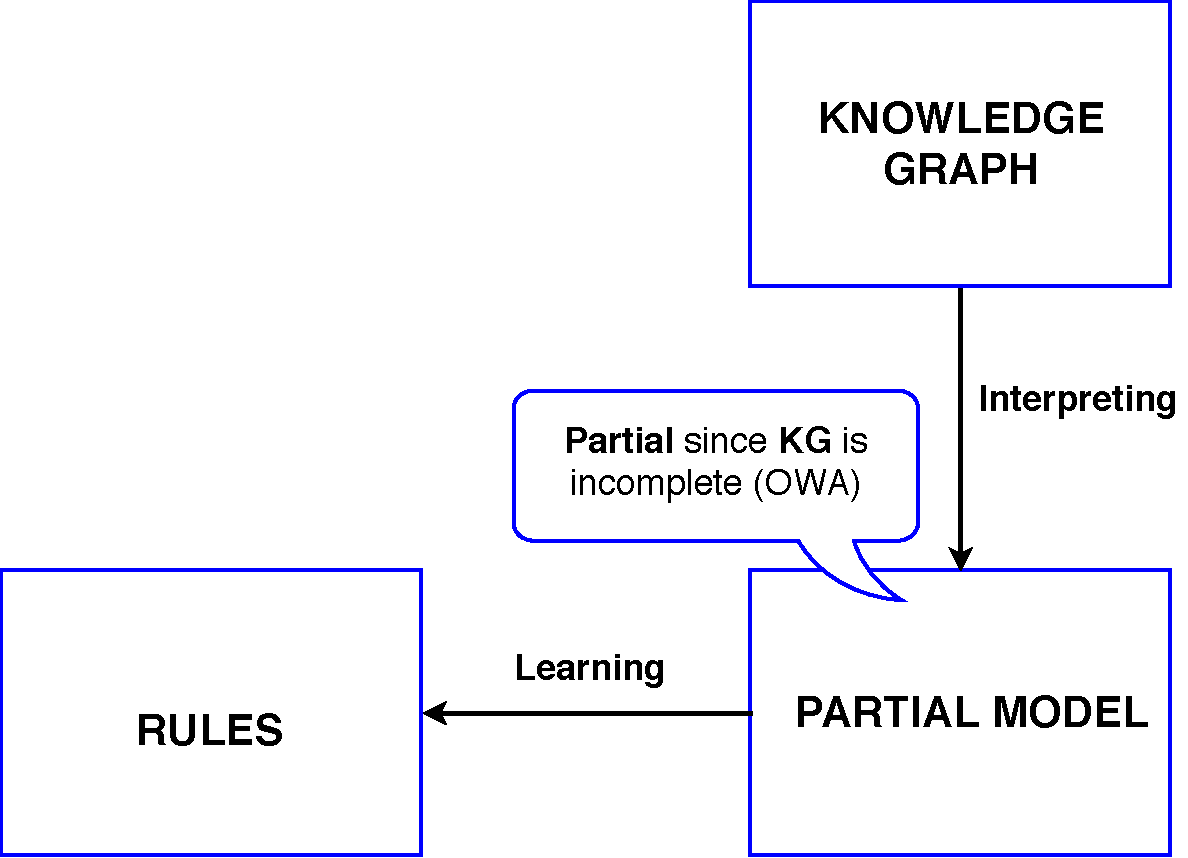
\includegraphics[width=0.86\textwidth]{asp_3}}
% \end{picture}}
% \end{frame}


\begin{frame}\frametitle{Horn Theory Revision}
\bigskip

 \begin{beamerboxesrounded}[upper=uppercolblue,lower=lowercolblue,shadow=true]{\textbf{\bl{Quality-based Horn Theory Revision}}}

 \smallskip

 \textbf{Given:} 
 \begin{itemize}
 \item Available KG 
\uncover<2->{ \item Horn rule set}
 \end{itemize}

\bigskip
\bigskip
\bigskip
\bigskip
\bigskip

 \uncover<3->{\noindent \textbf{Find:} }
 \begin{itemize}
\uncover<3->{ \item Nonmonotonic revision of Horn rule set}\uncover<4->{\\ with better 
 predictive quality}
 \end{itemize}
 \end{beamerboxesrounded}
\begin{picture}(0.5,0.5)\put(143,45){\alt<4>{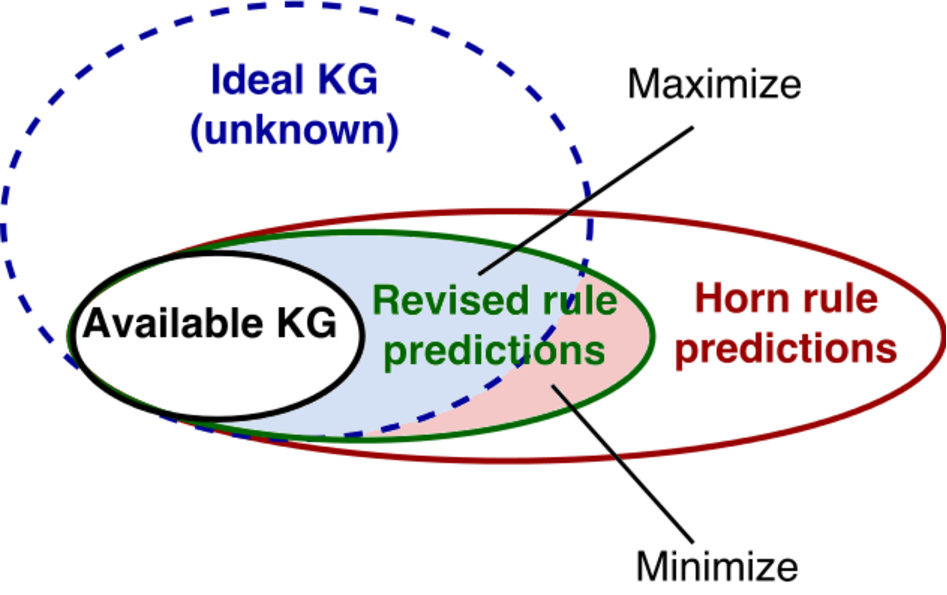
\includegraphics[width=0.58\textwidth]{big_pic_4}}{\alt<3>{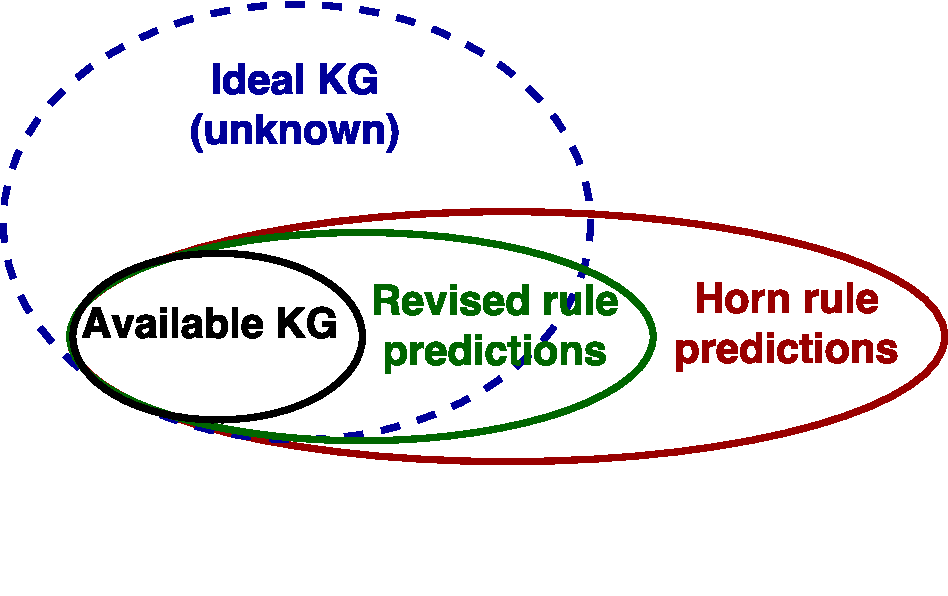
\includegraphics[width=0.58\textwidth]{big_pic_3}}{\alt<2>{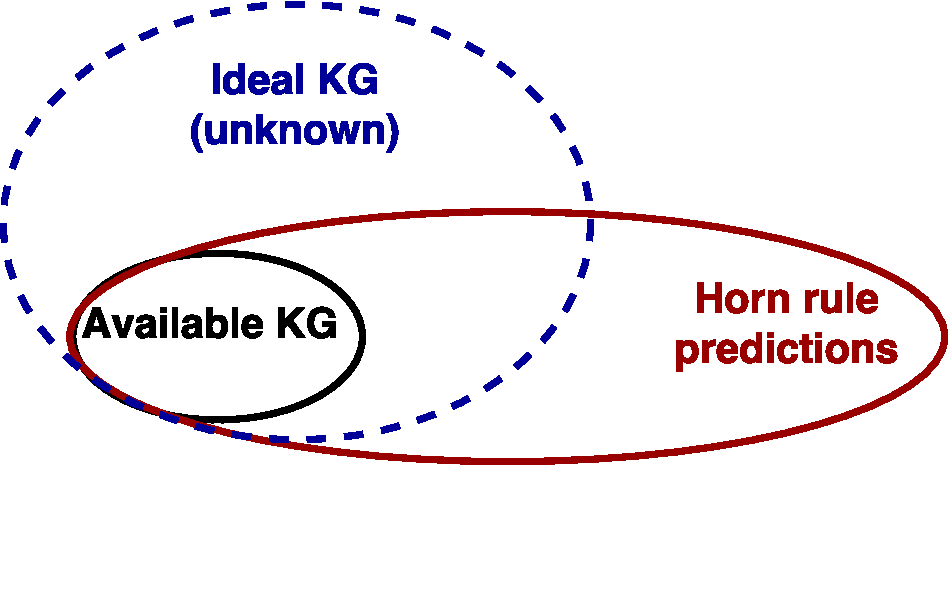
\includegraphics[width=0.58\textwidth]{big_pic_2}}{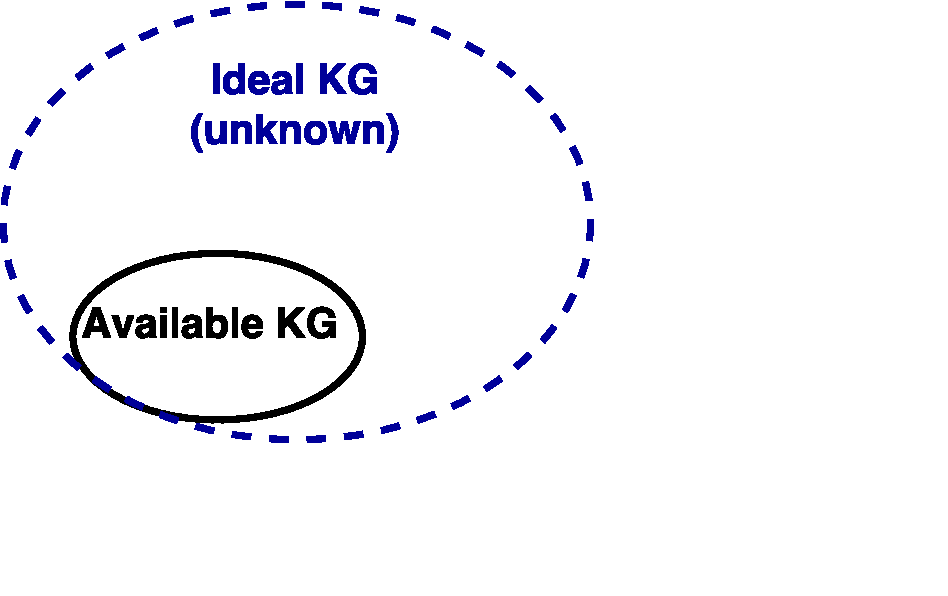
\includegraphics[width=0.58\textwidth]{big_pic_1}}}}}\end{picture}
\end{frame}

\begin{frame}\frametitle{Avoid Data Overfitting}
\begin{beamerboxesrounded}[upper=uppercolgreen,lower=lowercolgreen,shadow=true]{How to distinguish exceptions from noise?}\bigskip

\small{$
            \renewcommand{\arraystretch}{1.1}
             \begin{array}{@{\,}l@{~~}l@{}}
               \mi{\gr{r1:\,livesIn(X,Z) \leftarrow isMarriedTo(Y,X),livesIn(Y,Z),}\, \alert{\naf\ researcher(X)}}\\
              \visible<2->{\phantom{r1:\,}\mi{\,not\_livesIn(X,Z) \leftarrow isMarriedTo(Y,X),livesIn(Y,Z),researcher(X)}\\[2.75ex]}
              \visible<3->{\mi{\gr{r2:\,livesIn(X,Z)\leftarrow bornIn(X,Z),\,}\alert{\naf\ moved(X)}}}\\
              \visible<3->{\phantom{r1:\,}\mi{\,not\_livesIn(X,Z)}\leftarrow bornIn(X,Z),moved(X)}
             \end{array}$\bigskip

\uncover<4>{$\{\gr{\mi{livesIn(c,d)}},\mi{not\_livesIn(c,d)}\}$ are conflicting predictions\bigskip

\textbf{Intuition:} Rules with good exceptions should make few conflicting predictions
}}
\end{beamerboxesrounded}
\end{frame}

\begin{frame}\frametitle{Horn Theory Revision}

\bigskip

 \begin{beamerboxesrounded}[upper=uppercolblue,lower=lowercolblue,shadow=true]{\textbf{\bl{Quality-based Horn Theory Revision}}}

 \smallskip

 \textbf{Given:} 
 \begin{itemize}
 \item Available KG 
 \item Horn rule set
 \end{itemize}

\bigskip
\bigskip
\bigskip
\bigskip
\bigskip

 \noindent \textbf{Find:} 
 \begin{itemize}
 \item Nonmonotonic revision of Horn rules, such that \\
\begin{itemize}
\item number of \bl{conflicting predictions} is \textbf{minimal} \smallskip

\item average \bl{conviction} %$\mi{conv(r,\text{KG})=\dfrac{1-supp(r,\text{KG})}{1-conf(r,\text{KG})}}$ 
is \textbf{maximal}
\end{itemize}
 \end{itemize}
 \end{beamerboxesrounded}
\begin{picture}(0.5,0.5)\put(143,68){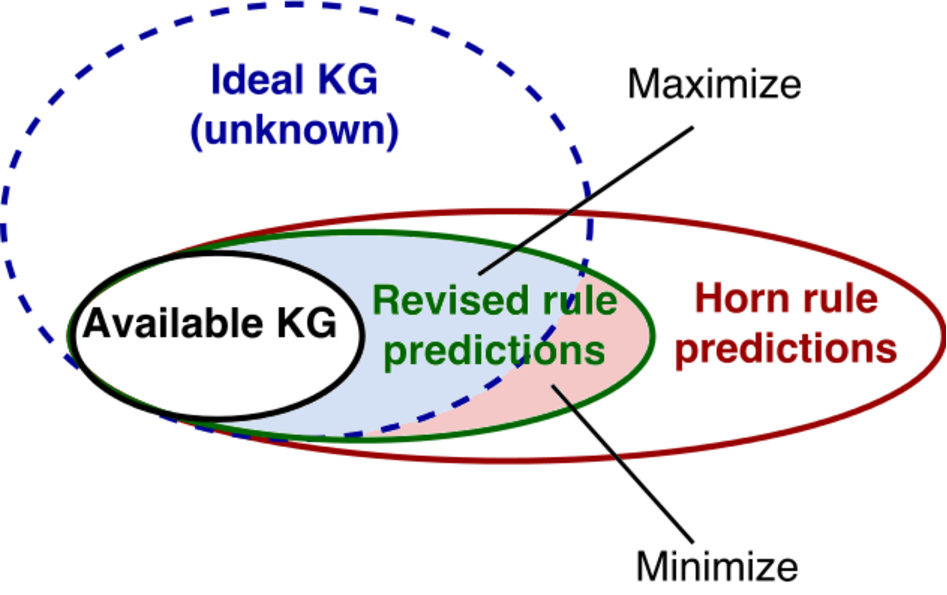
\includegraphics[width=0.58\textwidth]{big_pic_4}}\end{picture}
%\textcolor{gray}{\tiny{M. Gad-Elrab, D. Stepanova, J. Urbani, G. Weikum. Exception-enriched Rule Learning from Knowledge Graphs, ISWC 2016}}
\end{frame}


\begin{frame}\frametitle{Approach Description}
\begin{center}
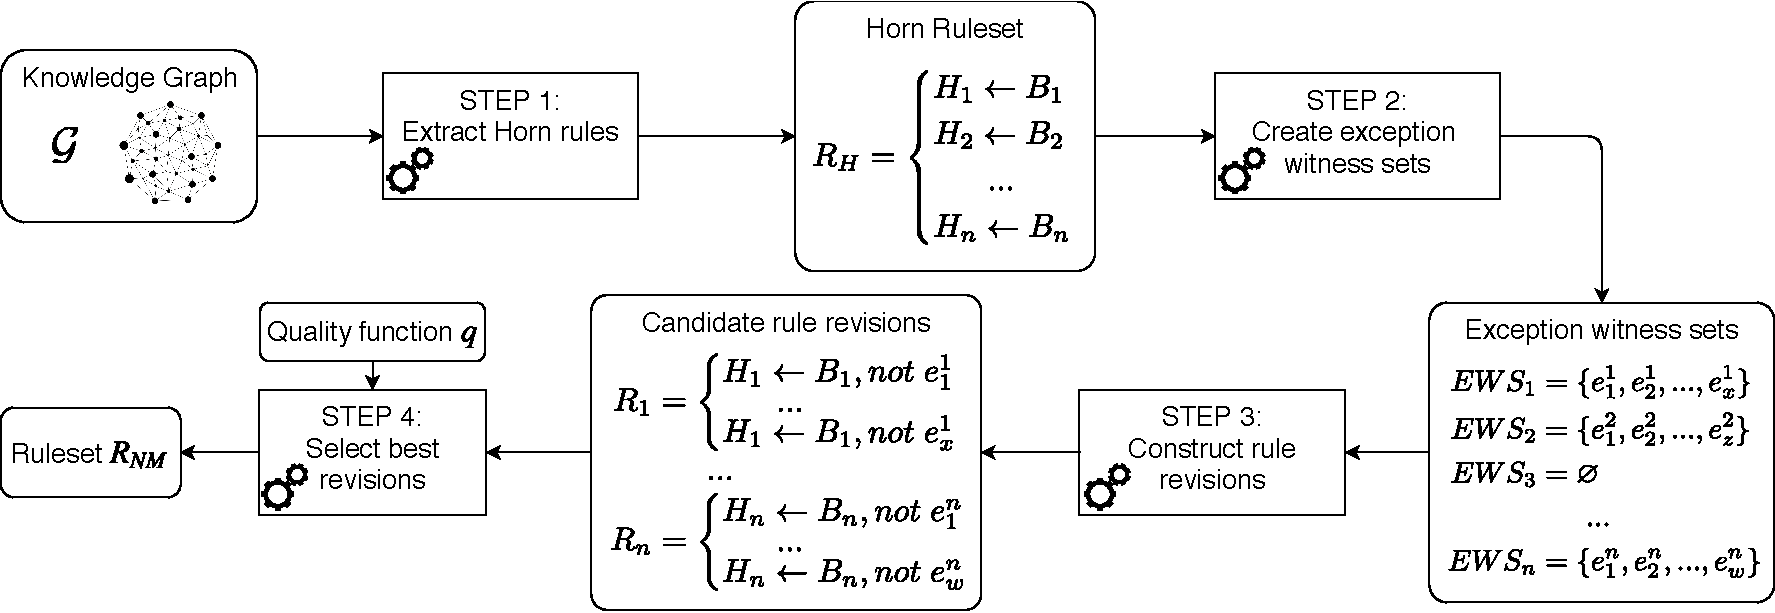
\includegraphics[width=1\textwidth]{nrl}
\end{center}
\end{frame}


\begin{frame}\frametitle{Exception Candidates}
\begin{picture}(0.5,0.5)\put(40,-183,5){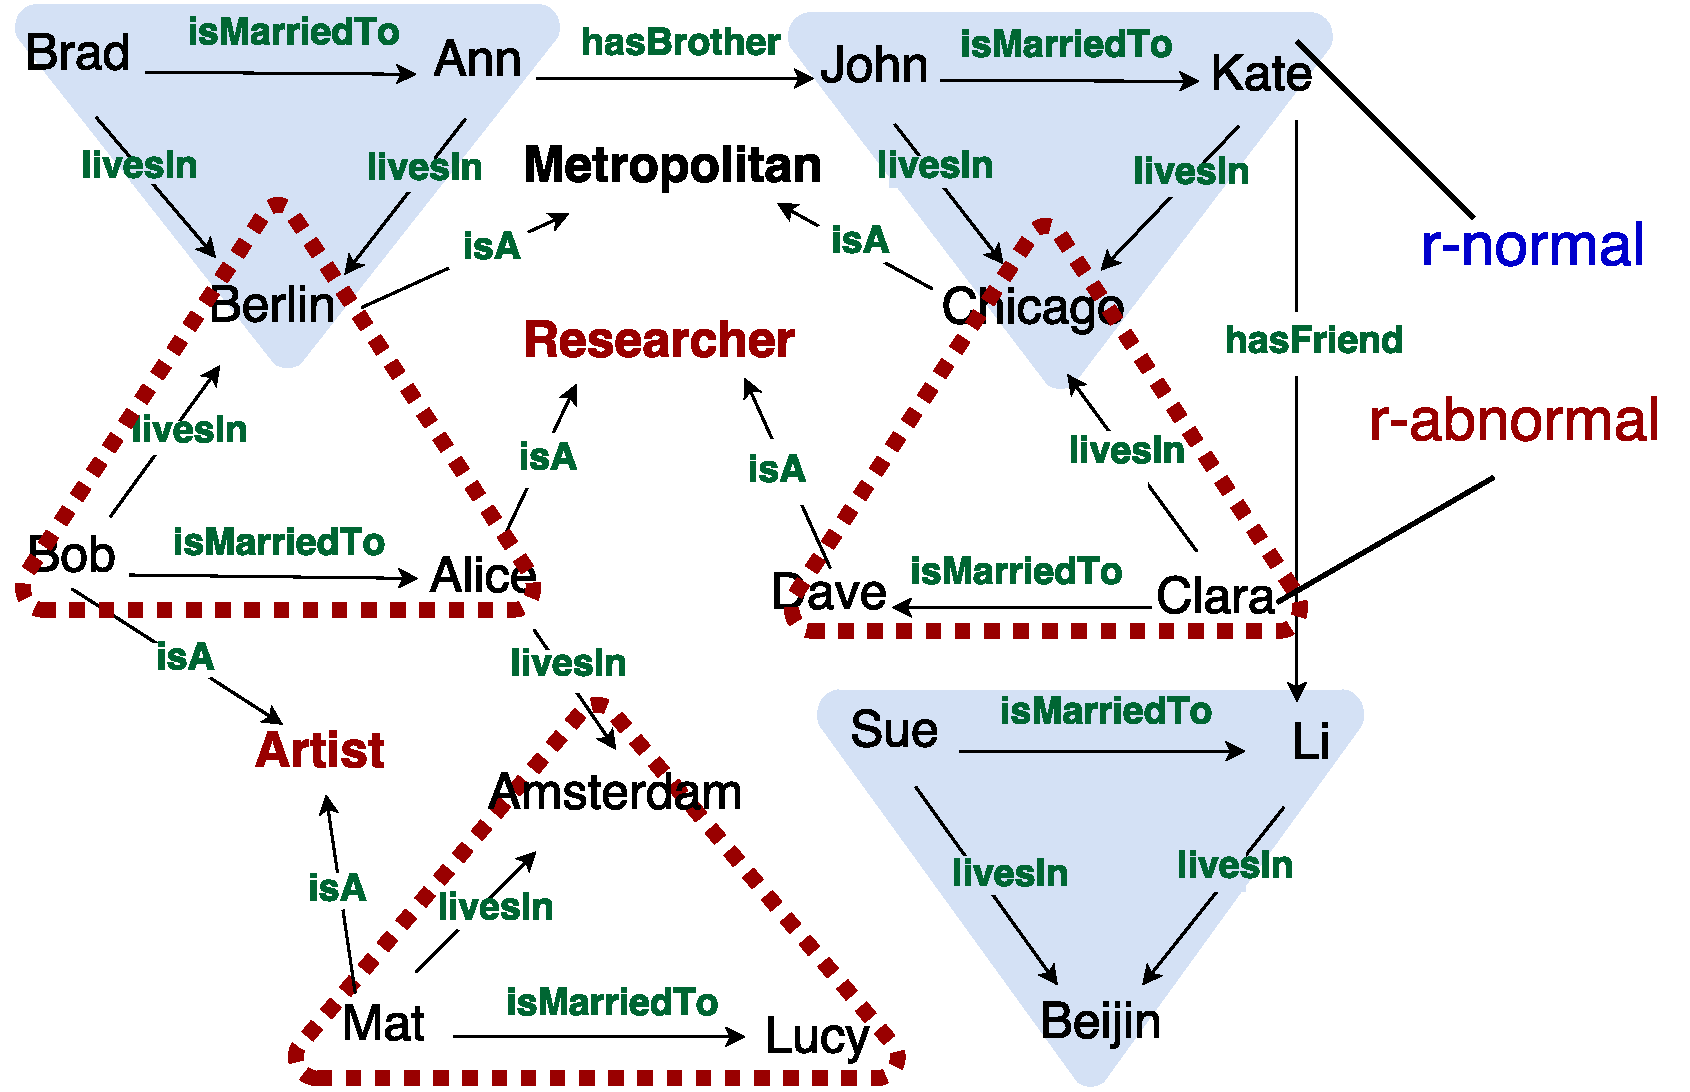
\includegraphics[width=0.75\textwidth]{kg_advanced3}}
\end{picture}
\bigskip
\bigskip
\bigskip
\bigskip
\bigskip
\bigskip
\bigskip
\bigskip
\bigskip
\bigskip
\bigskip
\bigskip
\bigskip
\bigskip
\bigskip
\bigskip
\bigskip


\leftline{\gr{$r{:}\,\mi{livesIn(X,Z)}\,{\leftarrow}\, \mi{isMarriedTo(Y,X)\,{,}\,livesIn(Y,Z)}$}}
\FrameText{\alert{$\left\{\begin{array}{@{}l@{}}
 \mbox{}\small{\mi{{\naf}\,researcher(X)}}\\
\mbox{}\small{\mi{{\naf}\,artist(Y)}}\end{array}\right\}$}}
\end{frame}



\begin{frame}\frametitle{Exception Ranking}

\begin{center}
$\mi{\gr{rule1}\;\;\; \alert{\{\underline{\mathbf{e_1}},e_2,e_3, \dotsc\}}}$\\
 $\mi{\gr{rule2}\;\;\; \alert{\{e_1,\underline{\mathbf{e_2}},e_3, \dotsc\}}}$\\
 $\mi{\gr{rule3}\;\;\; \alert{\{\underline{\mathbf{e_1}},e_2,e_3, \dotsc\}}}$\\
\end{center}

\begin{beamerboxesrounded}[upper=uppercolred,lower=lowercolred,shadow=true]{}
\small{Finding globally best revision is expensive, exponentially many candidates!}
\end{beamerboxesrounded}
\begin{itemize}


\item \bl{Naive ranking:} for every rule inject exception that results in the highest conviction
\medskip

\item \bl{Partial materialization (PM):} apply all rules apart from a given one, inject exception that results in the highest average conviction of the rule and its rewriting

% \only<2>{
% $\gr{r1 \dotsc \dotsc \dotsc} \{\alert{\underline{\mathbf{e_1}},e_2,e_3, \dotsc}\}$\\
% \hilight{$\gr{r2 \dotsc \dotsc \dotsc} \{\alert{e_1,e_2,e_3, \dotsc}\}$\\
% $\gr{r3 \dotsc \dotsc \dotsc} \{\alert{e_1,e_2,e_3, \dotsc}\}$\\}}

\medskip

\item \bl{Ordered PM (OPM):} same as PM plus ordered rules application
\medskip

\item \bl{Weighted OPM:} same as OPM plus weights on predictions
\end{itemize}
\bigskip

\tiny{M. Gad-Elrab, D. Stepanova, J. Urbani, G. Weikum. Exception-enriched Rule Learning from Knowledge Graphs. \emph{ISWC2016}}\\
\tiny{D. Tran{,}\,D. Stepanova{,}\,M. Gad-Elrab{,}\,F. Lisi{,}\,G. Weikum. Towards Nonmonotonic Relational Learning from KGs{.}\,\emph{ILP2016}}
\end{frame}

\begin{frame}\frametitle{Experimental Setup}
\vspace{-.4cm}
\begin{itemize}
\item \bl{Approximated ideal KG}: original KG 
\smallskip

\item \bl{Available KG}: for every relation randomly remove 20\% of facts from approximated ideal KG
\smallskip

\item \bl{Horn rules}: $\mi{h(X,Y)\leftarrow p(X,Z),q(Z,Y)}$ 
\smallskip

\item \bl{Exceptions}: $\mi{e_1(X),e_2(Y),e_3(X,Y)}$
\smallskip

\item \bl{Predictions} are computed using \bl{answer set solver} DLV % \footnote{\tiny{\url{http://dlvsystem.com}}}
\end{itemize}
\bigskip
\bigskip
\bigskip
\bigskip
\bigskip
\bigskip
\bigskip
\bigskip
\bigskip
\bigskip
\bigskip

\bigskip
\bigskip

\visible<1>{\begin{picture}(0.5,0.5)\put(55,63){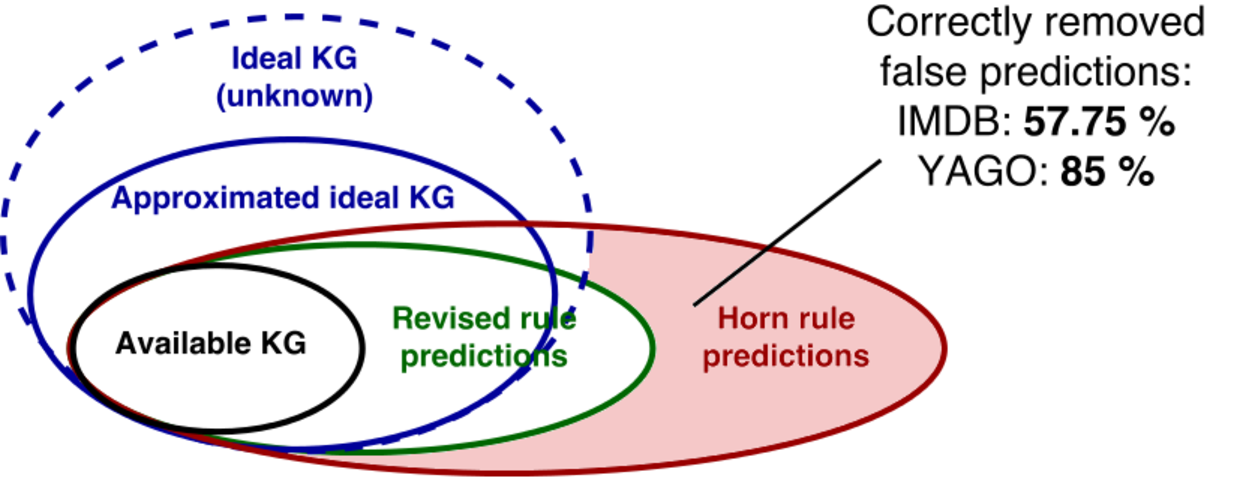
\includegraphics[width=0.75\textwidth]{big_pic_exp}}
\end{picture}}

\visible<2>{\vspace{-5,5cm}\begin{beamerboxesrounded}[upper=uppercolgreen,lower=lowercolgreen,shadow=true]{\textbf{Examples of revised rules:}}

 \begin{tabular}{l}
\footnotesize{

Plots of films in a sequel are written by the same writer, unless a film is American}\\
        \footnotesize{$\gr{r_1:  \mi{writtenBy(X, Z)}  \leftarrow
        \mi{hasPredecessor(X, Y)},\mi{writtenBy(Y, Z)},}$ \alert{$ not$  $\mi{american\_film(X)} $}}\\   
\\     
\footnotesize{
Spouses of film directors appear on the cast, unless they are silent film actors
}\\
      \footnotesize{ 
$\gr{r_2:  \mi{actedIn(X, Z)}  \leftarrow
        \mi{isMarriedTo(X, Y)},\mi{directed(Y, Z)},}$ \alert{$ not$  $\mi{silent\_film\_actor(X)} $}} \\
    
 \end{tabular} 
\end{beamerboxesrounded}      }



\end{frame}

\section{Incompleteness}

\begin{frame}\frametitle{Completeness-aware Rule Mining}
\begin{itemize}
\item Exploit \bl{cardinality meta-data} \cite{card} in \bl{rule mining}\\
\emph{\gr{John has \textbf{5} children, Mary is a citizen of \textbf{2} countries}}
\end{itemize}
\bigskip\bigskip
\bigskip
\bigskip
\bigskip
\bigskip
\bigskip
\bigskip
\bigskip
\bigskip
\bigskip

\begin{picture}(0.5,0.5)\put(40,-26){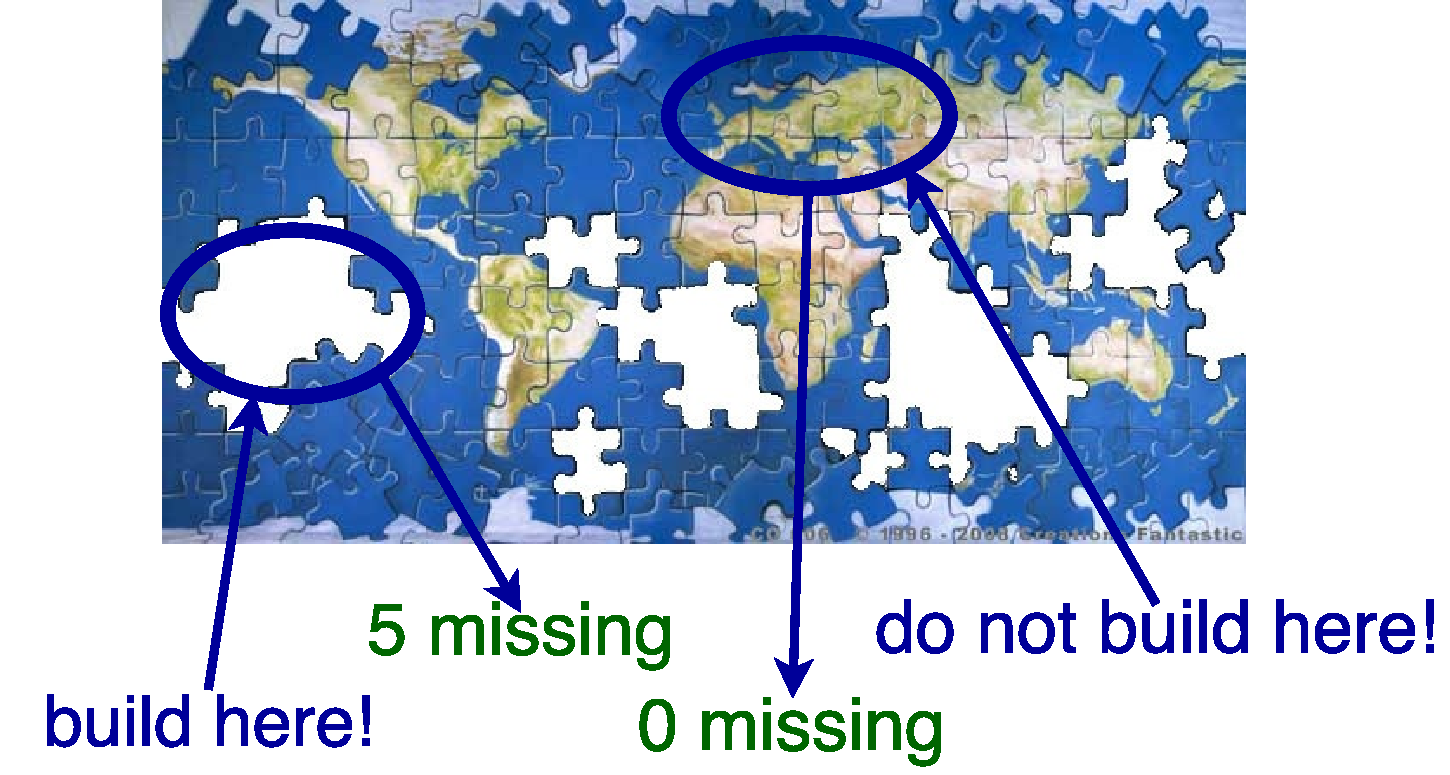
\includegraphics[width=0.8\textwidth]{worldmap}}
\end{picture}


\bigskip
\bigskip
\bigskip
\bigskip

\tiny{In Proc. ISWC 2017, Completeness-aware Rule Learning from Knolwegde Graphs. T. Pellissier-Tanon, D. Stepanova, S. Razniewski, P. Mirza, G. Weikum, 2018.}
\end{frame}

\begin{frame}\frametitle{Reasonable Rules}
\bigskip

\uncover<2->{
\small{\emph{\gr{ \uncover<3->{$\checkmark$} People with the same parents are likely siblings}}}
}

\uncover<4->{\alt<4>{
\bl{Closed World Assumption (CWA)}: all children of Alice are known
}{
\small{\bl{Partial Completeness A. (PCA)}: if a child of Alice is known, then all children are known}}}
\uncover<5->{\cite{amie}}

\alt<-2>{
\begin{picture}(0.5,0.5)\put(-5,-145){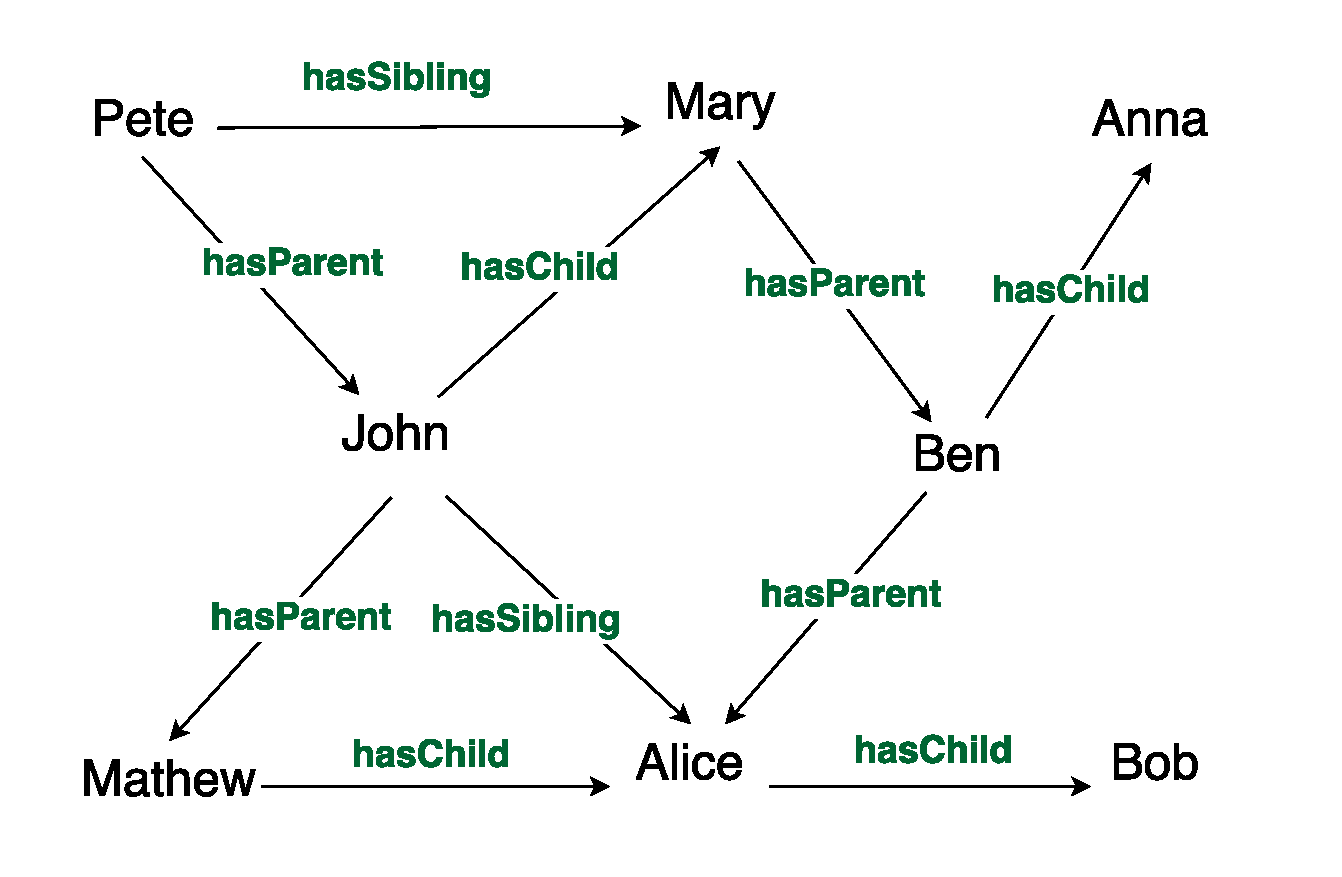
\includegraphics[width=.6\textwidth]{kg_sibl1}}\end{picture}
}{\alt<3>{
\begin{picture}(0.5,0.5)\put(-5,-145){\includegraphics[width=.6\textwidth]{kg_sibl3}}\end{picture}
}{
\begin{picture}(0.5,0.5)\put(-5,-145){\includegraphics[width=.6\textwidth]{kg_sibl2}}\end{picture}
}}

\bigskip
\bigskip
\bigskip
\bigskip
\bigskip
\bigskip
\uncover<4->{\rightline{\gr{$\mi{conf(r_1)}=\dfrac{|\myfilledtriangle{lightblue}|}{|\myfilledtriangle{lightblue}|+|\mytriangle{darkred}{white}|}=\dfrac{2}{4}$}}}
\bigskip

\uncover<5->{
\rightline{\gr{$\mi{conf_{pca}(r_1)}=\dfrac{|\myfilledtriangle{lightblue}|}{{\scriptstyle |\{\mytriangle{black}{white} \mid \mi{hasChild}(Z, \_)\in \cG\}|}}=\dfrac{2}{2}$}}}
\bigskip
\bigskip
\bigskip
\bigskip
\bigskip
\bigskip
\bigskip
\uncover<2->{\centerline{\gr{$\mi{r_1:\;hasSibling(Z,Y) \leftarrow hasChild(X,Y),hasParent(Z,X)}$}}}
\bigskip
\end{frame}


\begin{frame}\frametitle{Erroneous Rules due to Data Bias}
\bigskip

\uncover<2->{
\small{\emph{\uncover<3->{\textbf{\huge{\alert{$\times$}}}}\normalsize{\gr{People working and studying at the same institute are likely relatives}}}}
}

\alt<1>{\begin{picture}(0.5,0.5)\put(-5,-145){\includegraphics[width=.6\textwidth]{kg_works0}}
\end{picture}}{\alt<2>{\begin{picture}(0.5,0.5)\put(-5,-145){\includegraphics[width=.6\textwidth]{kg_works2}}
\end{picture}}{\begin{picture}(0.5,0.5)\put(-5,-145){\includegraphics[width=.6\textwidth]{kg_works1}}
\end{picture}}}

\bigskip
\bigskip
\bigskip
\bigskip
\bigskip
\uncover<3->{\rightline{$\gr{\mi{conf(r_2)}=\dfrac{|\myfilledtriangle{lightblue}|}{|\myfilledtriangle{lightblue}|+|\mytriangle{darkred}{white}|}=\dfrac{2}{4}}$}}
\bigskip

\uncover<3->{\rightline{$\gr{\mi{conf_{pca}(r_2)}=\dfrac{|\myfilledtriangle{lightblue}|}{{\scriptstyle |\{\mytriangle{black}{white} \mid \mi{hasSibling}(Z, \_)\in \cG\}|}}=\dfrac{2}{2}}$}}

\bigskip
\bigskip
\bigskip
\bigskip
\bigskip
\bigskip
\uncover<2->{\centerline{\gr{$\mi{r_2:\;hasChild(X,Z)\leftarrow worksAt(X,Y),educatedAt(Z,Y)}$}}}

\end{frame}



\begin{frame}\frametitle{Exploiting Meta-data in Rule Learning}
\bigskip

\begin{beamerboxesrounded}[upper=uppercolblue,lower=lowercolblue,shadow=true]
{}\begin{center}\textbf{\bl{Goal:}} make use of cardinality constraints on edges of the KG to improve rule learning. \end{center}
\end{beamerboxesrounded}
\bigskip
\bigskip
\bigskip
\bigskip
\bigskip
\bigskip
\bigskip\bigskip
\bigskip
\bigskip
\bigskip

\bigskip

\begin{picture}(0.5,0.5)\put(40,-10){\includegraphics[width=0.83\textwidth]{problem_pic}}
\end{picture}
\bigskip
\bigskip

\end{frame}

\begin{frame}\frametitle{Cardinality Statements}

\begin{itemize}
\item \bl{$\mi{num(p, s)}$}: Number of outgoing \bl{$p$}-edges from \bl{$s$} in the ideal KG
\item \bl{$\mi{miss(p,s)}$}: Number of missing \bl{$p$}-edges from \bl{$s$} in the available KG
\item If \bl{$\mi{miss(p,s)}=0$}, then \bl{$\mi{complete(p,s)}$}, otherwise \bl{$\mi{incomplete(p,s)}$}
\end{itemize}
\bigskip
\bigskip
\bigskip
\bigskip
\bigskip

\begin{columns}
\begin{column}{0.59\textwidth}
\begin{picture}(0.5,0.5)\put(10,-57){\includegraphics[width=\textwidth]{ex1}}\end{picture}
\end{column}
\begin{column}{0.39\textwidth}
\gr{$\mi{\;\;num(hasChild, john)=3}$}\\
\gr{$\mi{\;\;miss(hasChild,john)=1}$}\\
\gr{$\mi{\;\;incomplete(hasChild,john)}$}
\end{column}
\end{columns}
\end{frame}


\begin{frame}\frametitle{Cardinality Constraints on Edges}
\begin{itemize}
\item \bl{Mining cardinality assertions from the Web} \cite{cardinality-extraction-iswc-2016}
\begin{itemize}
\item \emph{\textcolor{darkgreen}{``... John has \textbf{2} children ...''}}
\end{itemize}
\bigskip


\item \bl{Estimating recall of KGs by crowd sourcing} \cite{whatknow}
\begin{itemize}
\item \emph{\textcolor{darkgreen}{20 \% of Nobel laureates in physics are missing}}
\end{itemize}
\bigskip

\item \bl{Predicting completeness in KGs} \cite{galarragapredicting}
\begin{itemize}
\item \gr{Add $\mi{complete(john,hasChild)}$ to KG and mine rules}
\\\emph{\textcolor{darkgreen}{$\mi{complete(X, hasChild) \leftarrow child(X)}$}}
\end{itemize}
\end{itemize}
\end{frame}


\begin{frame}\frametitle{Related Work}
\begin{picture}(0.5,0.5)\put(2,-120){\includegraphics[width=1.01\textwidth]{relwork}}
\end{picture}
\end{frame}


\begin{frame}\frametitle{Prediction Post-processing}
Remove predictions in complete KG parts \small{\cite{galarragapredicting}}, \\
\small{i.e., constraints are set on the output not the input}

\alt<3->{\begin{picture}(0.5,0.5)\put(35,-170){\includegraphics[width=0.75\textwidth]{complapp_1_3}}
\end{picture}}{\alt<2>{\begin{picture}(0.5,0.5)\put(35,-170){\includegraphics[width=0.75\textwidth]{complapp_1_2}}
\end{picture}}{\begin{picture}(0.5,0.5)\put(35,-170){\includegraphics[width=0.75\textwidth]{complapp_1_1}}
\end{picture}}}

\bigskip
\bigskip
\bigskip
\bigskip
\bigskip
\bigskip
\bigskip
\bigskip
\bigskip
\bigskip
\bigskip
\bigskip
\bigskip
\bigskip
\bigskip

\uncover<4>{
\begin{beamerboxesrounded}[upper=uppercolred,lower=lowercolred,shadow=true]
{}\begin{center}\textbf{\alert{Rules}} might be still \textbf{\alert{erroneous}}.. What about other incorrect predictions? \end{center}
\end{beamerboxesrounded}
}

\end{frame}

 

\begin{frame}\frametitle{Problem Statement}
\bl{\textbf{Given:}} 
\begin{itemize}
\item KG
\item numerical statements
\end{itemize}
\bigskip
\bigskip
\bigskip
\bigskip
\bigskip 
\bigskip 


\bl{\textbf{Find:}} \textbf{\gr{rules}} which predict
\begin{itemize}
\item ``few'' facts in \textbf{\textcolor{gray}{complete areas}}
\item ``many'' facts in \textbf{\textcolor{gray}{incomplete areas}}
\end{itemize}
\begin{picture}(0.5,0.5)\put(162,22){\includegraphics[width=0.55\textwidth]{compl1}}\end{picture}
\bigskip
\begin{beamerboxesrounded}[upper=uppercolblue,lower=lowercolblue,shadow=true]
{}\begin{center}\textbf{\bl{Intuition:}} rank rules by taking into account numerical constraints on edge counts  in the ideal KG\end{center}
\end{beamerboxesrounded}
\end{frame}
\begin{frame}\frametitle{Rule Predictions}
\bl{$\mi{npi}(r)$}: number of facts added to incomplete areas by $r$

\bl{$\mi{npc}(r)$}: number of facts added to complete areas by $r$

\uncover<2->{
\begin{picture}(0.5,0.5)\put(-13,-165){\includegraphics[width=.6\textwidth]{kg_siblmiss}}
\end{picture}

\bigskip
\bigskip
\bigskip
\bigskip
\bigskip
\bigskip
\bigskip
\bigskip
\uncover<3->{
	\rightline{\gr{$npi(r_1) = 1$}}
    \rightline{\gr{$npc(r_1) = 0$}}
}


\bigskip
\bigskip
\bigskip
\bigskip
\bigskip
\bigskip
\uncover<3->{\centerline{\gr{$\mi{r_1:\;hasSibling(Z,Y) \leftarrow hasChild(X,Y),hasParent(Z,X)}$}}}
}
\end{frame}

\begin{frame}\frametitle{Completeness Confidence}
\bl{$\mi{conf_{comp}}$}: do not penalize rules that predict new facts in incomplete areas

\begin{center}
\large{$$\bl{\mi{conf_{comp}(r)=\dfrac{|\myfilledtriangle{lightblue}|}{|\myfilledtriangle{lightblue}|+|\mytriangle{darkred}{white}|-\mi{npi}(r)}}}$$}
\end{center}

\vfill

\begin{itemize}
\item Generalizes standard confidence ($miss(r) = 0$)
\item Generalizes PCA confidence ($miss(r) \in \{ 0, +\infty\}$)
\end{itemize}

\end{frame}


\begin{frame}\frametitle{Completeness Confidence Example 1}

\begin{picture}(0.5,0.5)\put(-13,-165){\includegraphics[width=.6\textwidth]{kg_siblmiss}}
\end{picture}

\bigskip
\bigskip
\bigskip
\bigskip

\bigskip
\bigskip
 \uncover<2->{\rightline{\gr{$\mi{conf(r_1)}=\dfrac{|\myfilledtriangle{lightblue}|}{|\myfilledtriangle{lightblue}|+|\mytriangle{darkred}{white}|}=\dfrac{2}{4}$}}}
 \bigskip

 \uncover<2->{\rightline{\gr{$\mi{conf_{pca}(r_1)}=\dfrac{|\myfilledtriangle{lightblue}|}{{\scriptstyle |\{\mytriangle{black}{white} \mid \mi{hasSibling}(Z, \_)\in \cG\}|}}=\dfrac{2}{2}$}}}

\bigskip
\uncover<3->{\rightline{\gr{$npi(r_1) = 1$}}}
\bigskip

\uncover<3->{\rightline{\gr{$\mi{conf_{comp}(r_1)}=\dfrac{|\myfilledtriangle{lightblue}|}{|\myfilledtriangle{lightblue}|+|\mytriangle{darkred}{white}| - npi(r_1)}=\dfrac{2}{3}$}}}

\bigskip
\uncover<2->{\centerline{\gr{$\mi{r_1:\;hasSibling(Z,Y) \leftarrow hasChild(X,Y),hasParent(Z,X)}$}}}
\end{frame}

\begin{frame}\frametitle{Completeness Confidence Example 2}
\bigskip

\gr{$miss(hasChild, Alice) = 0$}

\begin{picture}(0.5,0.5)\put(-10,-135){\includegraphics[width=.6\textwidth]{kg_works1}}
\end{picture}

\bigskip
\bigskip
\bigskip
\uncover<2->{\rightline{\gr{$\mi{conf(r_2)}=\dfrac{|\myfilledtriangle{lightblue}|}{|\myfilledtriangle{lightblue}|+|\mytriangle{darkred}{white}|}=\dfrac{2}{4}$}}}
\bigskip

\uncover<2->{\rightline{\gr{$\mi{conf_{pca}(r_2)}=\dfrac{|\myfilledtriangle{lightblue}|}{{\scriptstyle |\{\mytriangle{black}{white} \mid \mi{hasChild}(Z, \_) \in \mathcal{G}\}|}}=\dfrac{2}{2}$}}}

\bigskip
\uncover<3->{\rightline{\gr{$npi(r_2) = 0$}}}
\bigskip

\uncover<3->{\rightline{\gr{$\mi{conf_{comp}(r_2)}=\dfrac{|\myfilledtriangle{lightblue}|}{|\myfilledtriangle{lightblue}|+|\mytriangle{darkred}{white}| - npi(r_2)}=\dfrac{2}{4}$}}}

\bigskip
\uncover<2->{\centerline{\gr{$\mi{r_2:\;hasChild(X,Z)\leftarrow worksAt(X,Y),educatedAt(Z,Y)}$}}}
\end{frame}

\begin{frame}\frametitle{Other Measures}
\bigskip

\bl{$\mi{precision_{comp}:}$} penalize $r$ that predict facts in complete areas
\begin{center}
 \bl{$\mi{precision_{comp}(r)} = 1 - \dfrac{\mi{npc}(r)}{|\myfilledtriangle{lightblue}|+|\mytriangle{darkred}{white}|}$ }
\end{center}
\bigskip

\bl{$\mi{recall_{comp}:}$} ratio of missing facts filled by $r$
\begin{center}
\bl{ $\mi{recall_{comp}(r)} = \dfrac{\mi{npi}(r)}{\sum_s \mi{miss}(h, s)}$ }
\end{center}
\bigskip

\bl{$\mi{dir\_metric:}$} proportion of predictions in complete and incomplete parts
\begin{center}
 \bl{$\mi{dir\_metric}(r) = \dfrac{\mi{npi}(r)-\mi{npc}(r)}{2\cdot(\mi{npi}(r)+\mi{npc}(r))}+0.5$}
\end{center}
\bigskip

\bl{$\mi{wdm}:$} weighted combination of confidence and directional metric
\begin{center}
 \bl{$\mi{wdm}(r) = \beta \cdot \mi{conf}(r) + (1-\beta) \cdot \mi{dir\_metric}(r)$}
\end{center}
\end{frame}


\begin{frame}\frametitle{Experimental Setup}

\bl{2 Datasets:}
\begin{itemize}
\item WikidataPeople: 2.4M facts over 9 predicates from Wikidata
\item LUBM: Synthetic 1.2M facts
\end{itemize}
\smallskip

\uncover<1->{
\bl{Creation of ideal KG:}
\begin{itemize}
\item WikidataPeople: using hand made rules
\item LUBM: using the OWL ontology
\end{itemize}
}
\smallskip

\uncover<1->{
\bl{Steps:}
\begin{itemize}
\item Generate $num(p,x)$ using the ideal KG
\item Remove triples randomly to create the available KG
\item Mine $r(X,Z) \leftarrow p(X,Y), q(Y,Z)$ rules
\item Gold standard: ratio of facts generated in the ideal KG
\end{itemize}
}

\end{frame}


\begin{frame}\frametitle{Experimental Evaluation}
\begin{center}
\includegraphics[width=\textwidth]{graph2}
\end{center}
\end{frame}

\begin{frame}\frametitle{Cardinality statements mining}

\begin{itemize}
\item Introduce $p_{\geq k}(s)$ and $p_{\leq k}(s)$ for each $num(p,s)$
\item Introduce $p_{\geq |\{ o \mid (s,p,o) \in \mathcal{G}|}(s)$ for all $p$ and $s$
\item Use the background rules $p_{\geq k}(s) \leftarrow p_{\geq k+1}(s)$ and $p_{\leq k+1}(s) \leftarrow p_{\leq k}(s)$.
\item Mine rules which head is a $p_{\_}(\_)$
\item Complete the $\mathcal{G}$ with a confidence threshold
\item if $p_{\geq k}(s) \in \mathcal{G}_c$ and $p_{\leq k}(s) \in \mathcal{G}_c$ then $num(p,s)=k$
\end{itemize}
\end{frame}

\begin{frame}\frametitle{Completeness precision and recall}

We define a precision and a recall:
\begin{itemize}
\item[] $\mi{precision_{comp}(r)} = 1 - \frac{\mi{npc}(r)}{\mi{supp}(\mathbf{B})}$ (ratio of "complete" results)
\item[] $\mi{recall_{comp}(r)} = \frac{\mi{npi}(r)}{\sum_s \mi{miss}(h, s)}$ (ratio of "incomplete" results filled)
\end{itemize}
\end{frame}


\begin{frame}\frametitle{Example with precision and recall}
\begin{picture}(0.5,0.5)\put(15,-170){\includegraphics[width=.6\textwidth]{kg_sibl2}}
\end{picture}

\bigskip
\bigskip
\bigskip
\bigskip
\bigskip
\bigskip
\bigskip
\uncover<2->{\rightline{\bl{$npi(r) = 1$ $npc(r) = 0$}}}
\uncover<3->{\rightline{\gr{$\mi{precision_{comp}(r)}=1 - \frac{0}{4}=1$}}}
\uncover<4->{\rightline{\gr{$\mi{recall_{comp}(r)}=\frac{1}{2}$}}}

\bigskip
\bigskip
\bigskip
\bigskip
\bigskip
\bigskip
\bigskip
\centerline{\gr{$\mi{r:\;hasSibling(Z,Y) \leftarrow hasChild(X,Y),hasParent(Z,X)}$}}
\centerline{\bl{$miss(hasSibling, Mary) = 2$}}
\end{frame}

\begin{frame}\frametitle{Directional metric}
\begin{itemize}
\item[] $\mi{dir\_metric}(r) = \dfrac{\mi{npi}(r)-\mi{npc}(r)}{2\cdot(\mi{npi}(r)+\mi{npc}(r))}+0.5$
\item<2->[] \bl{Weighted:} $\mi{wdm}(r) = \beta \cdot \mi{conf}(r) + (1-\beta) \cdot \mi{dir\_metric}(r)$
\end{itemize}
\end{frame}

\begin{frame}\frametitle{Example with directional metric}
\begin{picture}(0.5,0.5)\put(15,-170){\includegraphics[width=.6\textwidth]{kg_sibl2}}
\end{picture}

\bigskip
\bigskip
\bigskip
\bigskip
\bigskip
\bigskip
\bigskip
\uncover<2->{\rightline{\bl{$npi(r) = 1$ $npc(r) = 0$}}}
\uncover<3->{\rightline{\gr{$\mi{dir\_metric}(r) = \frac{1-0}{2\cdot (1+0)}+0.5= 1$}}}
\uncover<4->{
	\rightline{\gr{$\mi{wdm}(r) = 0.5 \cdot \frac{2}{4} + 0.5 \cdot 1 = \frac{3}{4}$}}
	\rightline{$\beta = 0.5$}
}
\bigskip
\bigskip
\bigskip
\bigskip
\bigskip
\bigskip
\centerline{\gr{$\mi{r:\;hasSibling(Z,Y) \leftarrow hasChild(X,Y),hasParent(Z,X)}$}}
\centerline{\bl{$miss(hasSibling, Mary) = 2$} $\beta = 0.5$}
\end{frame}


\section{Rules from Hybrid Sources}
\begin{frame}\frametitle{Knowledge Graph Completion}
 \begin{beamerboxesrounded}[upper=uppercolbl,lower=lowercolbl,shadow=true]{}
\begin{itemize}
\item \textbf{Given:} a KG, i.e., set of \bl{$\tuple{s\;p\;o}$} facts and possibly text
\item \textbf{Find:} missing \bl{$\tuple{s\;p\;o}$} facts
\end{itemize}
\end{beamerboxesrounded}
\bigskip
\pause

\begin{columns}
\begin{column}{.5\textwidth}
 \begin{beamerboxesrounded}[upper=uppercolbl,lower=lowercolbl,shadow=true]{\begin{center}\small{\textbf{Rule-based approaches}}\end{center}}
\smallskip
\begin{center}
  \includegraphics[width=\linewidth]{rule-based2}
\medskip

\tiny{
AMIE \cite{amieplus}, \cite{excep}, \\ RUMIS \cite{rumis}, CARL \cite{carl}, etc.
}
\end{center}
 \end{beamerboxesrounded}
\end{column}
\pause
\begin{column}{.5\textwidth}
 \begin{beamerboxesrounded}[upper=uppercolbl,lower=lowercolbl,shadow=true]{\begin{center}\small{\textbf{Statistics-based approaches}}\end{center}}


\bigskip

\alt<4->{\includegraphics[width=\linewidth]{statistics-based2}}{\includegraphics[width=\linewidth]{statistics-based1}}
\medskip
\begin{center}
\tiny{TransE \cite{transe}, TEKE \cite{teke},\\ RESCAL \cite{rescal}, etc.}
\end{center}
\end{beamerboxesrounded}


\end{column}

\end{columns}
\end{frame}

\begin{frame}\frametitle{Motivation}
\medskip

 \begin{beamerboxesrounded}[upper=uppercolblue,lower=lowercolbl,shadow=true]{\begin{center}\small{\bl{\textbf{Goal:}} Combine available techniques into a hybrid method}\end{center}}
\bigskip

\begin{columns}
\begin{column}{.4\textwidth}
 \begin{beamerboxesrounded}[upper=uppercolbl,lower=lowercolbl,shadow=true]{\begin{center}\small{\textbf{Rule-based approaches}}\end{center}}
\medskip

\begin{itemize}
\item[\bl{+}] \bl{Interpretable}
\item[\bl{+}] \bl{Limited training data}
\item[\alert{-}] \alert{Local patterns}
\item[\alert{-}] \alert{Not extendable}
\end{itemize}
 \end{beamerboxesrounded}
\end{column}

\begin{column}{.4\textwidth}
 \begin{beamerboxesrounded}[upper=uppercolbl,lower=lowercolbl,shadow=true]{\begin{center}\small{\textbf{Statistics-based approaches}}\end{center}}
\medskip

\begin{itemize}
\item[\alert{-}] \alert{Hard to interpret}
\item[\alert{-}] \alert{A lot of training data}
\item[\bl{+}] \bl{Global patterns}
\item[\bl{+}] \bl{Extandable (e.g., text)}
\end{itemize}
\end{beamerboxesrounded}
\end{column}
\end{columns}
\bigskip

 \end{beamerboxesrounded}
\bigskip

 \begin{beamerboxesrounded}[upper=uppercolblue,lower=lowercolbl,shadow=true]{\begin{center}\small{\bl{\textbf{Proposed solution}}}\end{center}}
Precompute KG embedding and treat the result as an oracle, which can be queried any time during rule construction.
 \end{beamerboxesrounded}
\bigskip

\begin{center}\tiny{Vinh Thinh Ho, Daria Stepanova, Mohamed Gad-Elrab, Evgeny Kharlamov, Gerhard Weikum}\end{center}
\end{frame}




\begin{frame}\frametitle{Problem Statement}
 \begin{beamerboxesrounded}[upper=uppercolblue,lower=lowercolbl,shadow=true]{\textbf{\bl{Feedback-driven rule mining}}}

\begin{itemize}
\item \textbf{Given:} 
\begin{itemize}
\item KG 
\item Embedding model  
\item Form of rules to be learned (e.g.number of atoms, with(out) negation, etc.)
\end{itemize}
\bigskip

\item \textbf{Find:} 
\begin{itemize}
\item Set of rules of the desired type, which agree with embedding model
on predictions that they make
\end{itemize}
\end{itemize}
\end{beamerboxesrounded}
\end{frame}

\iffalse
	\begin{frame}\frametitle{Related Works}
	\begin{itemize}
	\item \textbf{\bl{Constraints in embedding models}}
	\begin{itemize}
	\item Injecting logical formulas as constraints into embedding models
	(output is still a set of predictions; unclear where they came from)
	\cite{DBLP:journals/corr/abs-1711-11231}
	\end{itemize}
	\bigskip
	\bigskip
	
	\item \textbf{\bl{Rule mining with external support}}
	\begin{itemize}
	
	\item Interactive pattern mining
	\cite{DBLP:conf/kdd/GoethalsMV11}, \\\cite{DBLP:conf/pakdd/DzyubaL17}\medskip
	
	\item Interactive association rule mining
	\cite{DBLP:conf/pkdd/SkrabalSVHMCK12}
	\end{itemize}
	\end{itemize}
	\end{frame}
\fi




\begin{frame}\frametitle{Mine-Interact-Learn-Repeat}
\small{\begin{itemize}
\item[] Mimic \bl{``mine-interact-learn-repeat''} schema \scriptsize{\cite{interpat}}
\uncover<2->{\item[] \small{Establish \bl{``user-in-the-loop''} inspired interaction between the
rule mining algorithm and the embedding model}}
\end{itemize}}
\begin{center}
  \includegraphics[width=.91\textwidth]{user_loop}
\end{center}
\uncover<2->{\begin{picture}(0.5,0.5)
\alt<3->{\put(281,55){\includegraphics[width=.215\textwidth]{blackbox}}
\end{picture}}{\put(292,45){\includegraphics[width=.37\textwidth]{kgembed}}
\end{picture}}
\begin{picture}(0.5,0.5)
\put(-15,70){\includegraphics[width=.25\textwidth]{kg}}
\end{picture}
\begin{picture}(0.5,0.5)
\put(105,-10){\includegraphics[width=.33\textwidth]{feedback}}
\end{picture}
\begin{picture}(0.5,0.5)
\put(125,124){\includegraphics[width=.195\textwidth]{rules}}
\end{picture}}
\end{frame}


\begin{frame}\frametitle{Research Questions}
\small{
\alt<4->{
 \begin{beamerboxesrounded}[upper=uppercolblue,lower=lowercolblue,shadow=true]{}
\begin{itemize}
\item[\bl{Q1}] \textbf{(Interact)} What kind of feedback is required/possible\\ to obtain from the ``black box''
to organize convenient and effective interaction process?
\end{itemize}
\end{beamerboxesrounded}}
{\begin{itemize}
\item[\bl{Q1}] \textbf{(Interact)} What kind of feedback is required/possible\\ to obtain from the ``black box''
to organize convenient and effective interaction process?
\end{itemize}}
\pause

\bigskip
\begin{itemize}
\item[\bl{Q2}] \textbf{(Mine)} How to adapt existing rule mining algorithms to account for feedback?
\bigskip
\pause

\item[\bl{Q3}] \textbf{(Learn)} Can anything be learnt from the feedback provided by embeddings?

\end{itemize}}
\end{frame}




\begin{frame}\frametitle{Embedding-based  Methods}
\begin{itemize}
\item \textbf{\bl{Intuition:}} For \bl{$\tuple{s,p,o}$} in KG, find \bl{$\mathbf{s,p,o}$} such that \bl{$\mathbf{s}+\mathbf{p}\approx \mathbf{o}$}
\item The ``error of translation'' of a true KG fact should be smaller by a certain margin than the ``error of translation'' of an out-of-KG one
%Embedding models output the quality of a given fact based on a 
%\vspace{-.2cm}
\medskip

\leftline{\alt<4>{\includegraphics[width=1.03\textwidth]{figures/kg_embed4}}{\alt<3>{\includegraphics[width=1.03\textwidth]{figures/kg_embed3}}{ \alt<2>{\includegraphics[width=1.03\textwidth]{figures/kg_embed2}}{\includegraphics[width=1.03\textwidth]{figures/kg_embed1}}}}}

%Used by embedding models to measure quality of a given fact (s,p,o).
% Corrupted set of facts:
% Rank of (s,p,o) is the number of unknown facts in its corrupted set, which
%have greater embedding score than (s,p,o).
 \end{itemize}
\end{frame}


\begin{frame}\frametitle{Q1 (Interact)}
Measure quality of \bl{ $r: \mi{p(X,Y)\leftarrow B}$}, based on the embedding model\bigskip

\begin{itemize}
% \item quality of a set of facts is defined using $\mi{mrr}$ measure
% \begin{center}
% \bl{$\mi{mrr(S)=\dfrac{1}{|S|}\sum\limits_{{<}s\,p\,o{>}\in S}rank({<}s\,p\,o{>})}$}
% \end{center}
% \bigskip

\item rely on average quality of predicted facts
\begin{center}
\bl{$\mi{rule\_mrr(r)}=\dfrac{1}{|predictions(r)|} \sum\limits_{{<}s\,p\,o{>}\in predictions(r)}\mi{rank({<}s\,p\,o{>})}$}
\end{center}
\end{itemize}
\bigskip
\pause

\begin{beamerboxesrounded}[upper=uppercolblue,lower=lowercolbl,shadow=true]{\bl{Example}}
\begin{center}\bl{$\mi{livesIn(X,Y)\leftarrow actedIn(X,Z),producedIn(Z,Y)}$}\end{center}
\vspace{-.3cm}
\begin{itemize}
%\item Facts in KG: $\mi{<Kate\,livesIn\,Chicago>}, \mi{<Bob\,livesIn\,Berlin>},... $
\item rule predictions: \bl{$\mi{{<}Jack\,livesIn\,NY{>}}$,
$\mi{{<}Mat\,livesIn\,Berlin{>}}$}
\end{itemize}
% \begin{columns}
% \begin{column}{.22\textwidth}

% \small{$\mi{<Kate\,livesIn\,Chicago>}$\\
% $\mi{<Bob\,livesIn\,Berlin>}$\bigskip

% $\mi{{<}\colorbox{lightbl}{Jack}\,\mathbf{\gr{livesIn}}\,\colorbox{lightgr}{NY}{>}}$\\
% $\mi{{<}\colorbox{lightbl}{Mat}\,\mathbf{\gr{livesIn}}\,\colorbox{lightgr}{Berlin}{>}}$
% }
% \end{column}
% \begin{column}{.77\textwidth}
% \vspace{-.7cm}
\begin{center}
\uncover<2>{\scriptsize{
$\bl{rule\_mrr(r){=}}\dfrac{\bl{rank(}{<}\colorbox{lightbl}{Jack}\,\mathbf{\gr{livesIn}}\,\colorbox{lightgr}{NY}{>}\bl{)}{\bl{+}}\bl{rank(}{<}\colorbox{lightbl}{Mat}\,\mathbf{\gr{livesIn}}\,\colorbox{lightgr}{Berlin}{>}\bl{)}}{\bl{2}}$}}
\end{center}
% \bigskip

% Rule predictions are in black
% \end{column}
% \end{columns}
\end{beamerboxesrounded}
\end{frame}




\begin{frame}\frametitle{Q1 (Interact)}
Measure quality of \bl{ $r: \mi{h(X,Y)\leftarrow B}$}, based on the embedding model\bigskip
\begin{itemize}
\item rely on average quality of predicted facts estimated by embeddings
\begin{center}
\bl{$\mi{rule\_mrr(r)}=\dfrac{1}{|N|} \sum\limits_{s,h,o\in N}\dfrac{1}{\mi{rank(s,h,o)}}$}
\end{center}
\bigskip

\item combination of mrr with standard rule measures over KG
\begin{center}
\bl{$\mi{embed\_conf(r)}=\lambda*conf(r)+(1-\lambda)*\mi{rule\_mrr(r)}$},
\end{center}
\begin{itemize}
\pause
\item \bl{$\lambda$}: a weighting factor
\item \bl{$\mi{conf}$}: descriptive quality based on the original KG \\
any other standard rule measure can be plugged in
\item \bl{$\mi{rule\_mrr}$}: predictive quality based on KG embedding\\
any embedding model including text-enhanced ones can be used
\end{itemize}

%\bigskip
%
%\item more complex interaction, e.g., information theoretic measures?

\end{itemize}

\end{frame}


\begin{frame}\frametitle{Research Questions}
\small{
\begin{itemize}
\item[\bl{Q1}] \textbf{(Interact)} What kind of feedback is required/possible\\ to obtain from the ``black box''
to organize convenient and effective interaction process?
\end{itemize}
\bigskip

\begin{beamerboxesrounded}[upper=uppercolbl,lower=lowercolblue,shadow=true]{}
\begin{itemize}
\item[\bl{Q2}] \textbf{(Mine)} How to adapt existing rule mining algorithms to account for feedback? 
\end{itemize}
\end{beamerboxesrounded}
\bigskip

\begin{itemize}
\item[\bl{Q3}] \textbf{(Learn)} Can anything be learnt from the feedback provided by embeddings?
\end{itemize}}
\end{frame}


\begin{frame}\frametitle{Q2 (Mine)}

\bl{\textbf{Tentative algorithm steps:}}

\begin{itemize}
\item maintain a rule queue, starting from an empty rule
\bigskip

\item for each rule:
\begin{itemize}
\item[1.] process the rule \\
\uncover<2->{- compute statistics: \bl{$\mi{rule\_mrr, embed\_conf}$}\\
- filter rules based on statistics and output rule}
\bigskip

\item[2.] extend the queue by applying refinement operators\\
\uncover<3->{- add dangling atom\\
- add closing atom\\
- add positive unary atom\\
- add exception unary atom\\
- add exception binary atom}
\end{itemize}

\end{itemize}

% Algorithm goal:
% \bigskip

% \begin{itemize} 
% \item \bl{\textbf{Input:}} KG, embedding model
% \bigskip

% \item \bl{\textbf{Output:}} rules with:
% \begin{itemize}
% \item  unary predicates
% \item  binary predicates
% \item negated atoms in the body
% \item disjunctions in the head
% \end{itemize} 
% \bigskip

% \item Follow top-down clause search based on refinement operators \cite{DBLP:journals/ml/Quinlan90}, \cite{amieplus}
% \medskip

% \item Query embedding model at every step before rule expansion
% \end{itemize}
% \begin{center}
% \end{center}
\end{frame}


\begin{frame}\frametitle{Refinement Operators}
%\begin{picture}(0.5,0.5)\put(-30,-100){
%\alt<3->{\includegraphics[width=1\textwidth]{figures/refinement_operators2}}{\alt<2->{\includegraphics[width=1\textwidth]{figures/refinement_operators1}}{\includegraphics[width=1\textwidth]{figures/refinement_operators0}}}}
%\end{picture}
\begin{picture}(0.5,0.5)\put(-52,-130){
\leftline{\includegraphics[width=1.3\textwidth]{refinement_operators3}}
}
\end{picture}
\bigskip
\bigskip
\bigskip
\bigskip
\bigskip
\bigskip\bigskip
\bigskip
\bigskip
\bigskip
\bigskip
\bigskip

\begin{beamerboxesrounded}[upper=uppercolbl,lower=lowercolblue,shadow=true]{}
\begin{itemize}
\item Exploit embedding to prune rule search space
\item Generate rule language bias dynamically
\end{itemize}
\end{beamerboxesrounded}
\end{frame}


\begin{frame}\frametitle{Research Questions}
\small{


\begin{itemize}
\item[\bl{Q1}] \textbf{(Interact)} What kind of feedback is required/possible\\ to obtain from the ``black box''
to organize convenient and effective interaction process?
\end{itemize}

\bigskip
\begin{itemize}
\item[\bl{Q2}] \textbf{(Mine)} How to adapt existing rule mining algorithms to account for feedback?
\end{itemize}
\bigskip

 \begin{beamerboxesrounded}[upper=uppercolblue,lower=lowercolblue,shadow=true]{}
\begin{itemize}
\item[\bl{Q3}] \textbf{(Learn)} Can anything be learnt from the feedback provided by embeddings?
\begin{itemize}
\item Ideally, we want to learn the structure of most promising rules, i.e., the best rules have at most 5 atoms, 4 variables, etc..
\medskip

\end{itemize}
\end{itemize}
\end{beamerboxesrounded}
}

\end{frame}
\begin{frame}\frametitle{Embedding-Based Hybrid Quality Function}
\captionsetup[subfigure]{font=evensmallerfont}
 \begin{figure}[t]
     \centering
     \vspace{-0.2cm}
     \subfloat{{\includegraphics[width=0.6\textwidth]{figures/new_exp1/legend-crop.pdf}}}\\
     \setcounter{subfigure}{0}
     \vspace{-0.25cm}
     \subfloat[Conf-HolE on FB15K]{{\includegraphics[width=0.27\textwidth,height=3.1cm]{figures/new_exp1/fb15k_hole_conf-crop.pdf} }\label{fig:fb-HoLE-Conf}}
     \subfloat[Conf-SSP on FB15K]
{{\includegraphics[width=0.27\textwidth,height=3.1cm]{figures/new_exp1/fb15k_ssp_conf-crop.pdf} \label{fig:fb-SSP-Conf}}}
    \subfloat[PCA-SSP on FB15K]
    {{\includegraphics[width=0.27\textwidth,height=3.1cm]{figures/new_exp1/fb15k_ssp_pca-crop.pdf} }\label{fig:fb-SSP-PCA}}\\
     \vspace{-0.25cm}
    \subfloat[Conf-TransE on Wiki44K]{{\includegraphics[width=0.27\textwidth,height=3.1cm]{figures/new_exp1/wiki44k_transe_conf-crop.pdf} }\label{fig:wi-TransE-Conf}}
    \subfloat[Conf-SSP on Wiki44K]{{\includegraphics[width=0.27\textwidth,height=3.1cm]{figures/new_exp1/wiki44k_ssp_conf-crop.pdf} }\label{fig:wi-SSP-Conf}}
     \subfloat[PCA-SSP on Wiki44K]{{\includegraphics[width=0.27\textwidth,height=3.1cm]{figures/new_exp1/wiki44k_ssp_pca-crop.pdf} }\label{fig:wi-SSP-PCA}} \\  

    
     %\caption{
     %$pred\_prec_{CW}$ of the \textit{top-k} rules with various $\lambda$ on FB15K.
     %}
     \label{fig:diff_lambda}
 \end{figure}
\end{frame}


\begin{frame}\frametitle{Embedding-Based Hybrid Quality Function}
\setlength\tabcolsep{0.2em}
\begin{table}[t]
\scriptsize
%\tiny
\centering
\begin{tabular}{c |r r r r |r r r r} 
 \multirow{3}{*}{\textbf{\textit{top-k}}} & \multicolumn{4}{c}{\textbf{FB15K}} & \multicolumn{4}{|c}{\textbf{Wiki44K}} \\
 \cmidrule{2-9}
 & \textbf{Conf}&  \textbf{PCA} & \textbf{Conf-HolE}& \textbf{Conf-SSP} &  \textbf{Conf}&  \textbf{PCA} & \textbf{Conf-TransE}& \textbf{Conf-SSP}\\
  & {\scriptsize($\lambda=0$)}  & {\scriptsize($\lambda=0$)} & {\scriptsize($\lambda=0.3$)} & {\scriptsize($\lambda=0.3$)} & {\scriptsize($\lambda=0$)} & {\scriptsize($\lambda=0$)} &{\scriptsize($\lambda=0.3$)} & {\scriptsize($\lambda=0.3$)}\\
 \midrule
 \textbf{5} & 0.800 & 0.638 & \textbf{1.000} & \textbf{1.000} & 0.800 & 0.402 & \textbf{0.995} & 0.968\\
\textbf{10} & 0.900 & 0.506 & \textbf{1.000} & \textbf{1.000} & 0.638 & 0.321 & 0.863 & \textbf{0.932} \\
\textbf{20} & 0.900 & 0.499 & 0.950 & \textbf{1.000} & 0.712 & 0.357 & 0.802 & \textbf{0.825}\\
\textbf{50} & 0.881 & 0.410 & 0.936 & \textbf{0.937} & 0.670 & 0.352 & \textbf{0.675} & 0.674 \\
\textbf{100} & 0.855 & 0.348 & 0.885 & \textbf{0.895} & \textbf{0.477} & 0.331 & 0.474 & 0.474\\
\textbf{200} & 0.842 & 0.355 & 0.870 & \textbf{0.875} & -- & -- & -- & -- \\
 \bottomrule
\end{tabular}
\caption*{Precision of the \textit{top-k} rules learned using different measures in CW setting.}
\label{table:avg_quality}
\vspace*{-3mm}
\end{table}


\end{frame}

\begin{frame}\frametitle{Horn Rule Learning}
\setlength\tabcolsep{0.2em}
\begin{table}[t]
\scriptsize
\centering
\begin{tabular}{c|r r|r r|r r|r r|r r|r r}

 \multirow{3}{*}{\textbf{\textit{top-k}}}&\multicolumn{6}{|c}{\textbf{FB15K}} & \multicolumn{6}{|c}{\textbf{Wiki44K}}\\
 \cmidrule{2-13}&\multicolumn{2}{|c}{\textbf{AMIE-PCA}}&\multicolumn{2}{|c|}{\textbf{AMIE-Conf}}&\multicolumn{2}{|c}{\textbf{RuLES}}&\multicolumn{2}{|c}{\textbf{AMIE-PCA}}&\multicolumn{2}{|c}{\textbf{AMIE-Conf}}&\multicolumn{2}{|c}{\textbf{RuLES}} \\
 & \textit{Facts} & \textit{Prec.} & \textit{Facts} & \textit{Prec.} & \textit{Facts} & \textit{Prec.} &\textit{Facts} & \textit{Prec.} &\textit{Facts} & \textit{Prec.} &\textit{Facts} & \textit{Prec.} \\
 \midrule
 \textbf{20} & 1029 & 0.28 & 82 & 0.63 & 44 & 1.00 & 185 & 0.73 & 91 & 0.95 & 3291 & 0.98\\
 \textbf{50} & 1716 & 0.43 & 190 & 0.74 & 186 & 0.92 & 47099 & 0.10 & 3594 & 0.95 & 6154 & 0.88 \\
\textbf{100} & 3085 & 0.65 & 255 & 0.78 & 539 & 0.80 & 56831 & 0.20 & 13870 & 0.83 & 13253 & 0.82 \\
\textbf{200} & 10586 & 0.62 & 1210 & 0.83 & 1205 & 0.88 & 82288 & 0.39 & 19538 & 0.72 & 20408 & 0.73 \\
\textbf{500} & 40050 & 0.51 & 2702 & 0.75 & 7124 & 0.95 & 219264 & 0.35 & 124836 & 0.23 & 128256 & 0.48 \\
 \bottomrule
\end{tabular}
\caption*{Precision of the \textit{top-k} rules generated by RuLES and AMIE in OW setting.}
\label{table:amie_vs_RuLES}
\vspace*{-3mm}
\end{table}


\end{frame}

\begin{frame}\frametitle{RuLES for Exception-Aware Rule Learning}
%!TEX root = ../main.tex

% \begin{table}[t]
% \centering
% \begin{tabular}{|r|r r|r r|r r|r r|}
%  \hline
%  \multirow{3}{*}{$top-k$}&\multicolumn{4}{|c|}{FB15K} & \multicolumn{4}{|c|}{WIKI44K}\\
%  \cline{2-9}&\multicolumn{2}{|c|}{RUMIS}&\multicolumn{2}{|c|}{RuLES}&\multicolumn{2}{|c|}{RUMIS}&\multicolumn{2}{|c|}{RuLES} \\
%  & $Avg.scr.$ & $Avg.inc.$ & $Avg.scr.$ & $Avg.inc.$& $Avg.scr.$ & $Avg.inc.$& $Avg.scr.$ & $Avg.inc.$ \\
%  \hline
%  20 & 0.791 & 0.024 & 1.000 & 0.047 & 0.743 & 0.067 & 0.803 & 0.024 \\
%  50 & 0.826 & 0.015 & 1.000 & 0.045 & 0.609 & 0.054 & 0.701 & 0.026 \\
% 100 & 0.859 & 0.026 & 0.990 & 0.047 & 0.417 & 0.033 & 0.539 & 0.011 \\
% 200 & 0.848 & 0.034 & 0.977 & 0.065 & 0.253 & 0.022 & 0.339 & 0.017 \\
% 500 & 0.745 & 0.043 & 0.958 & 0.079 & -- & -- & -- & -- \\
% \hline
% \end{tabular}
% \caption{Average prediction score of some top non-monotonic rules from RuLES vs RUMIS.}
% \label{table:exception_prediction_result}
% \vspace*{-3mm}
% \end{table}

%\begin{table}[t]
%\centering
%\begin{tabular}{|c|r r|r r|r r|r r|}
% \hline
% \multirow{3}{*}{\textbf{\textit{top-k}}}&\multicolumn{4}{|c|}{\textbf{FB15K}} & \multicolumn{4}{|c|}{\textbf{Wiki44K}}\\
% \cline{2-9}&\multicolumn{2}{|c|}{\textbf{RUMIS}}&\multicolumn{2}{|c|}{\textbf{RuLES}}&\multicolumn{2}{|c|}{\textbf{RUMIS}}&\multicolumn{2}{|c|}{\textbf{RuLES}} \\
% & $Facts$ & $Prec.$ & $Facts$ & $Prec.$& $Facts$ & $Prec.$& $Facts$ & $Prec.$ \\
% \hline
%\textbf{20} & 672 & 0.95 & 34 & 0.97 & 5844 & 0.93 & 5640 & 0.93 \\
%\textbf{50} & 1797 & 0.94 & 158 & 0.99 & 8585 & 0.83 & 13333 & 0.84 \\
%\textbf{100} & 2672 & 0.94 & 434 & 0.99 & 21081 & 0.76 & 25265 & 0.81 \\
%\textbf{200} & 4103 & 0.87 & 1155 & 0.96 & 50957 & 0.51 & 43677 & 0.67 \\
%\textbf{500} & 13439 & 0.76 & 5466 & 0.90 & -- & -- & -- & -- \\
%\hline
%\end{tabular}
%\caption{$pred\_prec_{OW}$ of the \textit{top-k} rules learned by RUMIS and RuLES.}
%\label{table:exception_prediction_result}
%\vspace*{-3mm}
%\end{table}
\setlength\tabcolsep{0.4em}

\begin{table}[t]
\scriptsize
\centering
\begin{tabular}{r|r r|r r|r r|r r}
 & \multicolumn{4}{c}{\textbf{FB15K}} & \multicolumn{4}{|c}{\textbf{Wiki44K}} \\
 \cmidrule{2-9}&\multicolumn{2}{c}{\textbf{RUMIS}}&\multicolumn{2}{|c}{\textbf{RuLES}}&\multicolumn{2}{c}{\textbf{RUMIS}}&\multicolumn{2}{|c}{\textbf{RuLES}} \\
\textbf{\textit{top-k}} & \emph{Facts} & \emph{Prec.} & \emph{Facts} & \emph{Prec.} & \emph{Facts} & \emph{Prec.}& \emph{Facts} & \emph{Prec.} \\
 \midrule
\textbf{20} & 672 & 0.95 & 34 & 0.97 & 5844 & 0.93 & 5640 & 0.93 \\
\textbf{50} & 1797 & 0.94 & 158 & 0.99 & 8585 & 0.83 & 13333 & 0.84 \\
\textbf{100} & 2672 & 0.94 & 434 & 0.99 & 21081 & 0.76 & 25265 & 0.81 \\
\textbf{200} & 4103 & 0.87 & 1155 & 0.96 & 50957 & 0.51 & 43677 & 0.67 \\
\textbf{500} & 13439 & 0.76 & 5466 & 0.90 & -- & -- & -- & -- \\
\bottomrule
\end{tabular}
\begin{tabular}{r | r r| r r | r r |r r}
 & \multicolumn{4}{c}{\textbf{FB15K}} & \multicolumn{4}{|c}{\textbf{Wiki44K}} \\
 \cmidrule{2-9}&\multicolumn{2}{c}{\textbf{RUMIS}}&\multicolumn{2}{|c}{\textbf{RuLES}}&\multicolumn{2}{|c}{\textbf{RUMIS}}&\multicolumn{2}{|c}{\textbf{RuLES}} \\
\textbf{\textit{top-k}} & \emph{Facts} & \emph{Prec.} & \emph{Facts} & \emph{Prec.} & \emph{Facts} & \emph{Prec.}& \emph{Facts} & \emph{Prec.} \\
 \midrule
\textbf{20} & 76 & 0.70 & 111 & 0.68 & 63 & 0.47 & 81 & 0.94 \\
\textbf{50} & 126 & 0.51 & 435 & 0.74 & 191 & 0.28 & 611 & 0.69 \\
\textbf{100} & 183 & 0.43 & 680 & 0.76 & 543 & 0.49 & 1698 & 0.79 \\
\textbf{200} & 310 & 0.30 & 1112 & 0.87 & 4861 & 0.40 & 3175 & 0.80 \\
\textbf{500} & 1155 & 0.53 & 3760 & 0.59 & -- & -- & -- & -- \\
\bottomrule
\end{tabular}

\caption{$pred\_prec_{OW}$ (top) and $rev\_prec_{OW}$ (bottom)
of the \textit{top-k} rules learned by RUMIS and RuLES.}
\label{table:exception_prediction_result}
\vspace*{-3mm}
\end{table}
\end{frame}

\section{Further Topics}

\begin{frame}\frametitle{Commonsense Rule Mining from Hybrid Sources}
\bigskip

 \includegraphics[width=.25\textwidth]{dog_in_car}\uncover<2->{\includegraphics[width=.25\textwidth]{car_in_garage}}\uncover<3->{\includegraphics[width=.25\textwidth]{garage_in_house}}\uncover<4->{\includegraphics[width=.25\textwidth]{house_in_garden}}
\medskip

 \begin{columns}
 \begin{column}{.6\textwidth}
 \uncover<5->{\leftline{\includegraphics[width=.3\textwidth]{dog_in_garden}}}
%\vspace{-3.45cm}
\begin{picture}(0.5,0.5)\put(70,0){
\alt<7->{\includegraphics[width=.63\textwidth]{commonsense_kg1}}{\alt<6>{\includegraphics[width=.63\textwidth]{commonsense_kg2}}{\alt<5>{\includegraphics[width=.63\textwidth]{commonsense_kg3}}{\alt<4>{\includegraphics[width=.63\textwidth]{commonsense_kg4}}{\alt<3>{\includegraphics[width=.63\textwidth]{commonsense_kg5}}{\alt<2>{\includegraphics[width=.63\textwidth]{commonsense_kg6}}{\includegraphics[width=.63\textwidth]{commonsense_kg7}}}}}}}}
\end{picture}
% \end{column}
% \end{columns}
\uncover<7->{\begin{picture}(0.5,0.5)\put(60,85){\text{\large{\bl{+WebChild}}}}\end{picture}
}
\end{column}
\begin{column}{.4\textwidth}
% \uncover<8->{\begin{picture}(0.5,0.5)\put(160,130){\scriptsize{$\mi{larger(Y,X)\leftarrow in(X,Y)}$}}\end{picture}}
% \uncover<9->{\begin{picture}(0.5,0.5)\put(150,110){\scriptsize{$\mi{heavier(Y,X)\leftarrow on(X,Y)}$}}\end{picture}} 
% \uncover<10->{\begin{picture}(0.5,0.5)\put(130,90){\scriptsize{$\mi{has(X,wings) {\lor} round(X)\leftarrow in(X,sky)}$}}\end{picture}} 
% \uncover<10->{\begin{picture}(0.5,0.5)\put(180,80){\large{...}}\end{picture}} 
\uncover<8->{\begin{beamerboxesrounded}[upper=uppercolblue,lower=lowercolbl,shadow=true]{\textbf{\bl{Desired output:}}}
\scriptsize{\bl{$\mi{larger(Y,X)\leftarrow in(X,Y)}$\\
$\mi{heavier(Y,X)\leftarrow on(X,Y)}$\\
$\mi{has(X,wings) \lor round(X) \leftarrow in(X,sky)}$
\begin{center}$\dotsc$\end{center}
}}
\end{beamerboxesrounded}}
\end{column}
\end{columns}

%$\mi{heavier(Y,X)\leftarrow on(X,Y)}$ $\mi{has(X,wings)\leftarrow in(X,sky),flyingObject(X), not\;round(X)}$}\end{picture}}
\bigskip

\end{frame}

\begin{frame}\frametitle{Commonsense Rule Mining from Hybrid Sources (Text)}


\bigskip
\begin{itemize}

	\item Extracting rules from text challenges %as for~\cite{Schoenmackers:2010}
	\begin{itemize}
		\item Non-canonicalized, ambiguous and infinite set of relations.
		\item Noisy facts.
		\item Missing negative examples (OWA).
		
	\end{itemize}
\end{itemize}
\bigskip

\end{frame}

\begin{frame}\frametitle{Commonsense Rule Mining from Hybrid Sources (Text)}


\bigskip
\begin{itemize}

	\item \textbf{SHERLOCK}~\cite{Schoenmackers:2010}: Early attempt to learn rules from open domain text extractions.
	\item  \textbf{Golden et. al.}~\cite{Gordon:2011}: Utilizes presuppositional discourse patterns (such as statements with but, yet ... etc) to collect conditional knowledge in the form of \textit{if-then}.
  \item  \textbf{Dragoni et. al.}~\cite{Gordon:2011}: Extracts dependencies between text chunks in legal document such as contract. Then, these dependencies are converted into machine readable rules. 
  \item None of the existing work considered the combination between KGs and Text.
\end{itemize}
\bigskip

\end{frame}


\begin{frame}\frametitle{Rule Types}

\begin{itemize}
\item \textbf{Horn:} AMIE \cite{amieplus}\\
%\emph{Married people live together}\\
\bl{$\mi{livesIn(Z,Y)\leftarrow livesIn(X,Y), marriedTo(X,Z)}$}
\smallskip
\pause

\item \textbf{Nonmonotonic:} RUMIS \cite{excep}, \cite{rumis}\\ 
%\emph{Married people live together unless one is a researcher}\\
\bl{$\mi{livesIn(Z,Y)\leftarrow livesIn(X,Y), marriedTo(X,Z)}, not \;researcher(Z)$}
\smallskip
\pause

\item \textbf{Numerical:} CARL \cite{carl}\\
%\emph{If one has $\geq$ 4 siblings then one's parents have $\geq$ 5 children}\\
\bl{$\mi{hasChild_{\geq 5}(X) \leftarrow hasFather(Y,X), hasSibling_{\geq 4}(Y)}$}
\smallskip
\pause

\item \textbf{Disjunctive:} \\
%\emph{Actors from capitals are married to actors or politicians }\\
\bl{$\mi{male(Y) \lor female(Y)\leftarrow hasParent(X,Y)}$}
\pause

\item \textbf{Existential:} \\
\bl{$\mi{\exists Y\, hasParent(X,Y)\leftarrow person(X)}$}
\smallskip
\pause

\item \textbf{Temporal constraints:} \bl{$\mi{\bot \leftarrow bornIn(X,Y),after(Y,Z),studied(X,Z)}$}
%\gr{$\mi{}$}

\end{itemize}
\end{frame}


% %%%%%%%%%%%%%%%%%%%%%%%%%%%%%%%%%%%%%%%%%%%%%%%%%%%%%%%%%%%%%%%%%%%

% %\makeoverview
% \section{Ontologies and Rules}

% \begin{frame}\frametitle{Overview}
% \begin{itemize}
% \item[$\checkmark$] \bl{Motivation}
% \bigskip

% \item[] \textbf{\bl{Ontologies and Rules}}
% \bigskip

% \item[] \bl{Inconsistencies in DL-programs}
% \bigskip

% \item[] \bl{Nonmonotonic Rule Mining}
% \bigskip

% \item[] \bl{Further and Future Work}
% \end{itemize}
% \end{frame}


% %%%%%%%%%%%%%%%%%%%%%%%%%%%%%%%%%%%%%%%%%%%%%%%%%%%%%%%%%%%%%%%%%%%


% \begin{frame}
% \frametitle{History of Knowledge Representation}
% \small{\begin{itemize}
% \item \textbf{\bl{1950's:}} \bl{First Order Logic (FOL)} for KR (\alert{undecidable})\\
% (e.g. \cite{M59})
% \bigskip

% \item \textbf{\bl{1970's:}} \bl{Network-shaped structures} for KR (\alert{no formal semantics})\\
% (e.g. semantic networks \cite{semnet}, frames \cite{frames})
% \bigskip

% \item \textbf{\bl{1979:}} Encoding of \bl{network-shaped structures} into \bl{FOL} \cite{hayes79}
% \bigskip

% \item \textbf{\bl{1980's:}} \textcolor{blue}{Description Logics (DL)} for KR
% \begin{itemize}
% \item \bl{Decidable fragments} of \bl{FOL}
% \item Theories encoded in DLs are called \bl{ontologies}
% \item Many DLs with different expressiveness and computational features
% \item Particularly suited for \bl{conceptual reasoning}
% \end{itemize}
%  \end{itemize}}
% \end{frame}



% \begin{frame}
% \frametitle{Description Logic Ontologies}
% \textbf{\bl{Open World Assumption (OWA)}}: what is not derived is \bl{unknown}

%  \alt<2>{\begin{picture}(0.5,0.5)
%    \put(50,-136){\includegraphics[width=0.7\textwidth]{dl1}}
%   \end{picture}}{\begin{picture}(0.5,0.5)
%    \put(50,-136){\includegraphics[width=0.7\textwidth]{dl0}}
%   \end{picture}}
% \bigskip
% \bigskip
% \bigskip
% \bigskip
% \bigskip
% \bigskip
% \bigskip
% \bigskip
% \bigskip
% \bigskip
% \bigskip
% \bigskip
% \bigskip

% \begin{beamerboxesrounded}[upper=uppercolgreen,lower=lowercolgreen,shadow=true]{}
% \small{

% \textbf{Inclusions:} \gr{$\mi{Female \sqsubseteq \neg Male{,}hasSister \sqsubseteq hasSibling{,}hasBrother \sqsubseteq hasSibling}$}
% \smallskip
% \pause 

% \vspace{-.2cm}
% \textbf{Complex axioms:} \gr{\alt<2>{$\mi{Uncle \equiv Male \sqcap \exists hasSibling.\exists hasChild}$}{$\mi{\forall X\exists Y\,Z(Female(X) \wedge hasSibling(X,Y)\wedge hasChild(Y,Z))}$}}
% }
% \end{beamerboxesrounded}


% \end{frame}



% \begin{frame}\frametitle{What can not be said in DLs?}
% \begin{itemize}


% \item \bl{Exceptions} from theories (due to \bl{monotonicity})\\
% \end{itemize}
% \begin{center}
% \begin{columns}
% \begin{column}{.39\textwidth}
%  \uncover<2-4>{

%  $\gr{\mi{WithBeard \sqsubseteq Male}}$\\
%  $\gr{\mi{Female \sqsubseteq \neg Male}}$\\
%  $\gr{\mi{WithBeard(c)}}$\\
% }
%  \uncover<4->{\bl{$\mi{Female(c)}$\\}}
%  \uncover<2-4>{------------------------------------\\}
%  \uncover<3->{\gr{$\mi{Male(c)}$\\}}
%  \uncover<4->{\bl{$\neg \mi{Male(c)}$}\\}
% \end{column}
% \begin{column}{.39\textwidth}
%  \uncover<2-4>{

%  \emph{People with beards are male}\\
%  \emph{Female are not male}\\
%  \emph{C has a beard}\\
%  }
%  \uncover<4->{\emph{C is female}\\}
%  \uncover<2-4>{------------------------------------\\}
%  \uncover<3->{\emph{C is male}\\}
%  \uncover<4>{\emph{C is not male}\\}
% \end{column}
% \end{columns}
% \end{center}
% \uncover<4>{\begin{picture}(0.5,0.5)
%  \put(95,-10){\includegraphics[width=.25\textwidth]{malefemale}}
%  \end{picture}
% \bigskip

% \begin{center}\bl{Monotonicity:} the more we add, the more we get!\end{center}

% }
% \end{frame}


% \begin{frame}
%   \frametitle{History of Knowledge Representation}
% \bigskip
% \bigskip

% \begin{itemize}
% \item \textbf{\bl{1970's:}} \bl{Logic programming} \\(e.g. Prolog)
% \bigskip
% \bigskip

% \item \textbf{\bl{1980's:}} \bl{Nonmonotonic logics}\\ (e.g. circumscription \cite{DBLP:journals/ai/McCarthy80}, default logic \cite{DBLP:journals/ai/Reiter80})
% \bigskip
% \bigskip

% \item \bl{\textbf{1988:}} \bl{Nonmonotonic rules} under \bl{answer set semantics} (ASP) \\\cite{GL1988}
% \begin{itemize}
% \item \normalsize{Logic programs with \bl{model-based} semantics}
% \item \normalsize{\bl{Disjunctive datalog} with \bl{default negation} $\bl{\mi{not}}$}
% \end{itemize}

% \end{itemize}

% \end{frame}

% \begin{frame}\frametitle{Not is not $\neg$!}
%  \begin{beamerboxesrounded}[upper=uppercolgreen,lower=lowercolgreen,shadow=true]{\normalsize{\textbf{Default negation}} \large{\bl{$\naf$}} 
%    }
% \medskip

% At a rail road crossing cross the road if \textbf{no train is known} to approach\medskip

% \gr{$\mi{walk}\leftarrow \mi{at(X), crossing(X), \text{\emph{\textbf{not}} } train\_approaches(X)}$}

% \end{beamerboxesrounded}
% \bigskip
% \bigskip
% \bigskip

%  \begin{beamerboxesrounded}[upper=uppercolgreen,lower=lowercolgreen,shadow=true]{\normalsize{\textbf{Classical negation}}  \large{\bl{$\neg$}} 
%    }
% \medskip

% At a rail road crossing cross the road if \textbf{no train} approaches\medskip

% \gr{$\mi{walk}\leftarrow \mi{at(X), crossing(X), \neg train\_approaches(X)}$}
% \end{beamerboxesrounded}
% \end{frame}

% \begin{frame}\frametitle{Nonmonotonic Rules}
% \bigskip

% \bl{\textbf{Closed World Assumption (CWA):} } what is not derived is \bl{false}
% \bigskip
% \bigskip

% \small{ \bl{\textbf{Rule:} }
% $\underbrace{a_1 \lor \dotsc \lor a_k}_{\Large{\bl{\text{head}}}}\; \leftarrow\; \underbrace{b_1,\, \dotsc,\, b_m,\,\bl{not} \,b_{m+1},\,\dotsc,\,\bl{not} \,b_n}_{\bl{\text{body}}} $

% }
% \bigskip
% \bigskip

% \small{\bl{\textbf{Informal semantics:}} } If $b_1,\dotsc, b_{m}$ are true and \bl{none} of $b_{m+1},\dotsc,b_n$ is \bl{known}, \phantom{\textbf{Informal semantics:\;\;\;}}then at least one among $a_1,\dotsc, a_k$ must be true\bigskip
% \bigskip
% \bigskip

% \begin{beamerboxesrounded}[upper=uppercolgreen,lower=lowercolgreen,shadow=true]{}
% \small{
% \textbf{Default negation}: unless a child is adopted one of his parents must be female\medskip

% \gr{$\mi{female(Y)\lor female(Z)\leftarrow hasParent(X,Y),hasParent(X,Z),} \\
% \phantom{\mi{female(Y)\lor female(Z)\leftarrow}}\mi{Y \neq Z, \naf\,adopted(X)}$}
% \bigskip

% \textbf{Constraint:} ensure that no one is a parent of himself\medskip

% \gr{$ \bot \leftarrow \mi{parent(X,Y),parent(Y,X)}$}
% }

% \end{beamerboxesrounded}
% \bigskip

% \end{frame}


% %%%%%%%%%%%%%%%%%%%%%%%%%%%%%%%%%%%%%%%%%%%%%%%%%%%%%%%%%%%%%%%%%%%


% \begin{frame}
% \frametitle{Answer Set Programs}
% \begin{itemize}
% \item[]\uncover<1->{\bl{Evaluation} of ASP programs is model-based }%\footnote{unlike in prolog, which is based on theorem proving}}%\uncover<3->{, it consists of 2 steps:}
% \begin{itemize}
% \uncover<2->{\item[1.]\bl{Grounding}: substitute all \bl{variables with constants} in all possible ways }
% \uncover<4->{\item[2.]\bl{Solving}: compute a \bl{minimal model (answer set) $I$} satisfying all rules}
% \end{itemize}
% \end{itemize}
% \bigskip

% \begin{beamerboxesrounded}[upper=uppercolgreen,lower=lowercolgreen,shadow=true]{\textbf{Answer set program (ASP)} is a set of nonmonotonic rules}
% \bigskip

% $\gr{
%       \begin{array}{l@{\qquad}}
%          \mbox{(1) }\mi{hasParent(john,pat)}\;\;\; \mbox{(2) }\mi{hasParent(john,alex)}\;\;\;\mbox{(3) }\mi{male(alex)}\\[0.35ex]
%          \mbox{(4) }\mi{female(\alt<3->{\mi{pat}}{\bl{Y}})} \leftarrow \alt<3->{\mi{hasParent(john,pat)}}{\mi{hasParent(\bl{X,Y})}},\mi{hasParent(\alt<3->{john,alex}{\bl{X,Z}}),}\\
%          \phantom{\mbox{(4) }\mi{female(\alt<3->{pat}{\bl{Y}})\,} \leftarrow }\only<1,2>{\bl{Y\neq Z},} \mi{male(\alt<3->{alex}{\bl{Z}})},\naf\ \mi{adopted(\alt<3->{\mi{john}}{\bl{X}})} \uncover<5->{\\[0.35ex]\bl{\mbox{(5) }\mi{adopted(john)}}}
%       \end{array}
%     }$
% \medskip

% \uncover<5->{\small{$\phantom{\mi{I{=}\{\mi{hasParent(john,pat),hasParent(john,alex),male(alex)}}}\bl{\mi{adopted(john)}}$}}
% \uncover<4->{
% \small{$\gr{\mi{I{=}\{\mi{hasParent(john,pat),hasParent(john,alex),male(alex)},\alt<5>{\cancel{\mi{female(pat)}}}{\mi{female(pat)}}\}}}$}

% \uncover<4>{\medskip

% \bl{CWA:} \gr{$\mi{adopted(john)}$} can not be derived, thus it is false}}

% \end{beamerboxesrounded}


% \begin{center}\visible<5>{\bl{Nonmonotonicity}: adding facts might lead to loss of consequences!}\end{center}
% \end{frame}


%  \begin{frame}\frametitle{Combining Ontologies and Rules}
%  \begin{picture}(0.5,0.5)
% \alt<2>{\put(50,-130){\includegraphics[width=0.7\textwidth]{dlvsrules}}}{\put(50,-130){\includegraphics[width=0.7\textwidth]{dlvsrules0}}}
%  \end{picture}

%  \end{frame}

% \section{Inconsistencies in DL-programs}

% \begin{frame}\frametitle{Overview}
% \begin{itemize}
% \item[$\checkmark$] \bl{Motivation}
% \bigskip

% \item[$\checkmark$] \bl{Ontologies and Rules}
% \bigskip

% \item[] \textbf{\bl{Inconsistencies in DL-programs}}
% \bigskip


% \item[] \bl{Nonmonotonic Rule Mining}
% \bigskip

% \item[] \bl{Further and Future Work}
% \end{itemize}

% \begin{picture}(0.5,0.5)
% \put(200,65){\includegraphics[width=0.11\textwidth]{eiter}}
% \put(204,55){\text{\footnotesize{T. Eiter}}}
% \end{picture}

% \begin{picture}(0.5,0.5)
% \put(265,78){\includegraphics[width=0.095\textwidth]{fink}}
% \put(267,68){\text{\footnotesize{M. Fink}}}
% \end{picture}
% \end{frame}



% \begin{frame}\frametitle{DL-programs}
% \bl{DL-programs:} loose coupling of \bl{ontologies} and \bl{rules} \cite{EIL08}
% \bigskip
% \bigskip
% \bigskip
% \bigskip
% \bigskip
% \bigskip
% \bigskip
% \bigskip
% \bigskip
% \bigskip
% \bigskip
% \bigskip
% \bigskip
% \bigskip

% \begin{picture}(0.5,0.5)
% \put(80,-25){\includegraphics[width=0.53\textwidth]{dlp}}
% \end{picture}
% \end{frame}


% \begin{frame}\frametitle{\alt<15->{DL-program Repair}{\alt<14>{Inconsistent DL-program}{DL-program}}}
% \bigskip

% \small{
% \begin{beamerboxesrounded}[upper=uppercolgreen,lower=lowercolgreen,shadow=true]{\centerline{DL ontology}}
% \vspace{-.1cm}
%  \begin{columns}
%  \begin{column}{.38\textwidth}
% \begin{beamerboxesrounded}[upper=uppercolgreen,lower=lowercolgreen,shadow=true]{\centerline{Logical part}}
% \vspace{-.2cm}
% \gr{\begin{center}\small{$%O{=}\left\{
% \begin{array}{@{\,}l@{}}
%  \mbox{(1) }\mathit{Child \sqsubseteq \exists hasParent} \\[0.25ex]
%  \mbox{(2) }\mathit{Female \sqsubseteq \neg Male}  \\[0.25ex] 
% \mbox{(3) } \mathit{Adopted \sqsubseteq Child} \\[0.25ex]
%  \end{array}
% %\right\}
% $}
% \end{center}}
%  \end{beamerboxesrounded}
%  \end{column}
%  \begin{column}{.49\textwidth}
% \begin{beamerboxesrounded}[upper=uppercolgreen,lower=lowercolgreen,shadow=true]{\centerline{Data part (KG)}}
% \vspace{-.2cm}
% \gr{\begin{center}\small{$%O{=}\left\{
% \begin{array}{@{\,}l@{\,}l@{}}
%  \alt<16>{\bl{\mbox{(4) }\cancel{\mathit{Male(pat)}}\,\,\mathit{Female(pat)}}}{\alt<7>{\bl{\mbox{(4) }\mathit{Male(pat)}}}{\mbox{(4) }\mathit{Male(pat)}}}& \alt<15>{\bl{\mi{Female(alex)}}}{\alt<7>{\mi{Male(tim)}}{\uncover<6,7>{\bl{\mi{Male(tim)}}}}}\\[0.25ex]
%  \mbox{(5) }\mathit{Male(john)}&  \\[0.25ex] 
% \alt<17>{}{\alt<3>{\bl{\mbox{(6) }\mi{hasParent(john,pat)}}}{\mbox{(6) } \mathit{hasParent(john,pat)}}}& \\[0.25ex]
%  \end{array}
% %\right\}
% $}
% \end{center}}
%  \end{beamerboxesrounded}
%  \end{column}
% \end{columns}
% \end{beamerboxesrounded}
% }
% \bigskip

%  \begin{beamerboxesrounded}[upper=uppercolgreen,lower=lowercolgreen,shadow=true]{\centerline{Rules}}
%  \vspace{-.1cm}
% \gr{\small{\begin{center}
% $\begin{array}{@{\,}l@{~\,}}
% \alt<11>{\bl{ \mbox{(7) }\mi{isChildOf(john,alex)}}}{ \mbox{(7) }\mi{isChildOf(john,alex)}}\;\;\;\;\;\;\alt<6>{\bl{(8)\; \mi{boy(tim)}}}{(8)\; \mi{boy(tim)}}\\[0.35ex]
%  \mbox{(9) }\mi{hasFather}(john,pat) \leftarrow \alt<2->{\dlatom{}{\alt<3>{\bl{\mi{hasParent}}}{\mi{hasParent}}}{\alt<3>{\bl{\mi{john,pat}}}{\mi{john,pat}}}\only<3-8>{\;\;\bl{\checkmark}}}{\call}, \alt<4->{\\
% \phantom{\mbox{(9) }\mi{hasfather}(john,pat) \leftarrow}\;\; \dlatom{\alt<5,6>{\bl{\mi{Male} \uplus \mi{boy}}}{\mi{Male} \uplus \mi{boy}}}{\alt<7>{\bl{\mi{Male}}}{\mi{Male}}}{\alt<7>{\bl{\mi{pat}}}{\mi{pat}}}\only<7-8>{\;\;\bl{\checkmark}}}{\call}\\[0.35ex]
% \alt<14>{\alert{\mbox{(10) }\bot \leftarrow \mi{hasFather(john,pat),isChildOf(john,alex)},}\\
% \phantom{\mbox{(10) }\bot \leftarrow }\; \alert{\naf\dlatom{}{\mi{Adopted}}{john},}\\
% \phantom{\mbox{(10) }\bot \leftarrow }\; \alert{\naf\dlatom{\mi{Child}\uplus\mi{boy}}{\neg \mi{Male}}{\mi{alex}}}
% }{\alt<9->{\mbox{(10) }\bot \leftarrow \alt<10-14>{\bl{\mi{hasFather(john,pat)}}}{\mi{hasFather(john,pat)}},\alt<11-14>{\bl{\mi{isChildOf(john,alex)}}}{\mi{isChildOf(john,alex)}},\\
% \phantom{\mbox{(10) }\bot \leftarrow }\; \alt<12-14>{\bl{\naf\dlatom{}{\mi{Adopted}}{john}}}{\naf\dlatom{}{\mi{Adopted}}{john}},\\
% \phantom{\mbox{(10) }\bot \leftarrow }\; \alt<13-14>{\bl{\naf\dlatom{\mi{Child}\uplus\mi{boy}}{\neg \mi{Male}}{alex}}}{\naf\dlatom{\mi{Child}\uplus\mi{boy}}{\neg \mi{Male}}{alex}}\\}{}}
% \end{array}$%
%  \end{center}}}
%  \end{beamerboxesrounded}
%  \medskip

% \alt<15,16,17>{\bl{Repair answer set: }\gr{$\mi{I=\{isChildOf(john,alex),boy(tim)}\only<15>{\mi{,hasFather(john,pat)}}\}$}}{\alt<14>{\alert{\textbf{Inconsistent DL-program}: no answer sets!}}{\uncover<8>{\small{\bl{Answer set:} \gr{$\mi{I=\{isChildOf(john,alex),boy(tim),hasFather(john,pat)\}}$}}}}}



% \end{frame}


% \begin{frame}
% \frametitle{Inconsistency Handling in DL-programs}
% \bigskip

% \small{\bl{\textbf{Goal:}} develop techniques for handling inconsistencies in DL-programs}\\
% \small{\bl{\textbf{Approach:}} repair ontology data part (KG) to regain consistency}
% \smallskip

% \begin{center}
% \includegraphics[width=0.9\textwidth]{InconsisDLP}
% \end{center}

% \end{frame}




% \begin{frame}
% \frametitle{Complexity of Repair Answer Sets}
% \bigskip

% \begin{tabular}{|l|}
% \hline
% \small{\textbf{INSTANCE}: A ground DL-program $\Pi=\tuple{O,P}$.}\\
% \small{\textbf{QUESTION}: Does there exist a repair answer set for $\Pi$?} \\
% \hline
% \end{tabular}
% \bigskip

% \begin{theorem}
%  Deciding repair and standard answer set existence have the same complexity if instance query-answering in $O$ is polynomial ($\dllite_{\cA}, \el$).
%  \end{theorem}

% \begin{table}[ht]

% \centering 

% \begin{tabular}{| c | c | c |} 
% \hline
% \centering{\bl{$\Pi$}} & \bl{FLP semantics}& \bl{weak semantics}\\ [0.5ex] % inserts table
% %heading
% \hline 
% \bl{normal} &  \small{$\Sigma^P_2$-complete} &  \small{$\NP$-complete}\\ [1.5ex]% inserting body of the table
% \hline
% \bl{disjunctive} &  \small{$\Sigma^P_2$-complete}&  \small{$\Sigma^P_2$-complete}\\
% [1.5ex] 
% \hline
% \end{tabular}
% \label{table:nonlin} 
% \end{table}
% \bigskip
% \bigskip
% \bigskip


% \tiny{T. Eiter, M. Fink, D. Stepanova. Data Repair of Inconsistent DL-programs. \emph{IJCAI2013}}
% \\
% \tiny{T. Eiter, M. Fink, D. Stepanova. Data Repair of Inconsistent Nonmonotonic Description Logic Programs. \emph{JAI2016}}
% \end{frame}



% \begin{frame}\frametitle{Ontology Repair Problem}
% \bigskip

% \begin{tabular}{|l|}
% \hline
% \small{\textbf{INSTANCE}: Ontology $O$, \gr{$D_{\mi{true}}=\{\tuple{\mi{update,query}}\}$}, \alert{$D_{\mi{false}}=\{\tuple{update,query}\}$}}\\
% \small{\textbf{QUESTION}: Does there exist $O$ data part, for which queries under their}\\\phantom{\small{\textbf{QUESTION}:}} \small{updates from $\gr{D_{\mi{true}}}$ are true and from $\alert{D_{\mi{false}}}$ are false?} \\
% \hline
% \end{tabular}
% \bigskip

% \begin{theorem}
%  The Ontology Repair Problem is \NP-complete even if $O=\emptyset$.
%  \end{theorem}
% \bigskip

% \bl{Tractable cases:}
% \begin{itemize}
% \item Deletion repair
% \item Bounded addition
% \item Bounded change
% \item $\dotsc$
% \end{itemize}
% \end{frame}

% \begin{frame}
% \frametitle{Optimized DL-program Repair}

% \small{\begin{itemize}
% \item For each \bl{DL-atom} compute \bl{minimal sets of facts} (\sups), whose presence in ontology \bl{ensures DL-atom's query entailment} (small for some DLs)
% \uncover<2->{\item \bl{Guess values of DL-atoms} under which the program has an answer set}
% \uncover<3->{\item Solve \bl{ontology repair problem} as a variant of a \bl{hitting set problem}}
% \end{itemize}}
% \bigskip
% \bigskip
% \bigskip
% \bigskip
% \bigskip
% \bigskip
% \bigskip
% \bigskip
% \bigskip
% \bigskip
% \bigskip

% \begin{picture}(0.3,0.3)
%    \put(50,-5){\alt<3>{\includegraphics[width=.7\textwidth]{opt3}}{\alt<2>{\includegraphics[width=0.7\textwidth]{opt2}}{\includegraphics[width=.7\textwidth]{opt1}}}}
% \end{picture}
% \bigskip

% \uncover<3>{
% \tiny{T. Eiter, M. Fink, D. Stepanova. Towards Practical Deletion Repair of Inconsistent
% DL-programs. \emph{ECAI2014}}
% \\
% \tiny{T. Eiter, M. Fink, D. Stepanova. Computing Repairs for Inconsistent DL-programs
% over $\el$ Ontologies. \emph{JELIA2014, JAIR2016}}}

% \end{frame}


% \begin{frame}
% \frametitle{Example Benchmark}
% \begin{picture}(0.3,0.3)
%    \put(220,-30){\includegraphics[width=0.3\textwidth]{osm}}
% \end{picture}

% \bigskip
% \begin{itemize}
% \item \bl{Ontology:} MyITS\footnote{\tiny{http://www.kr.tuwien.ac.at/research/projects/myits/}}
% \begin{itemize}
% \item \bl{personalized route planning} with semantic
% information
% \smallskip

% \item logical axioms (406), (building features
% located inside private areas are not publicly accessible, covered
% bus stops are those with roofs) 
% \smallskip

% \item KG (4195 facts), Cork city map with leisure areas, bus stops,..
% \end{itemize}
% \bigskip


% \item \bl{Rules:} check that public stations don't lack public access, using \phantom{Rules:} CWA on private areas
% \bigskip

% \item \alert{Inconsistency:} wrong GPS coordinates result in roofed bus stops \phantom{Inconsistency:} being located inside private areas
% \bigskip

% \item \bl{Repair:} found within 12 seconds
% \end{itemize}
% \end{frame}


% \section{Nonmonotonic Rule Mining}


% \begin{frame}
% \frametitle{Overview}
% \begin{itemize}
% \item[$\checkmark$] \bl{Motivation}
% \bigskip

% \item[$\checkmark$] \bl{Ontologies and Rules}
% \bigskip

% \item[$\checkmark$] \bl{Inconsistencies in DL-programs}
% \bigskip

% \item[] \textbf{\bl{Nonmonotonic Rule Mining}}
% \bigskip

% \item[] \bl{Further and Future Work}
% \end{itemize}
% \begin{picture}(0.5,0.5)
% \put(170,45){\includegraphics[width=0.07\textwidth]{moh}}
% \put(163,35){\text{\tiny{M. Gad-Elrab}}}
% \end{picture}

% \begin{picture}(0.5,0.5)
% \put(202,58){\includegraphics[width=0.06\textwidth]{jacoppo}}
% \put(201,48){\text{\tiny{J. Urbani}}}
% \end{picture}

% \begin{picture}(0.5,0.5)
% \put(230,72){\includegraphics[width=0.065\textwidth]{weikum}}
% \put(227,62){\text{\tiny{G. Weikum}}}
% \end{picture}

% %\uncover<2>{
% \begin{picture}(0.5,0.5)
% \put(260,85.5){\includegraphics[width=0.08\textwidth]{tran}}
% \put(260,75.5){\text{\tiny{D. H. Tran}}}
% \end{picture}

% \begin{picture}(0.5,0.5)
% \put(292,98){\includegraphics[width=0.07\textwidth]{lisi}}
% \put(294,88){\text{\tiny{F. A. Lisi}}}
% \end{picture}
% %}
% \end{frame}


% \begin{frame}\frametitle{\alt<4>{Nonmonotonic Rule Mining}{Horn Rule Mining}}
% \smallskip

% \uncover<2->{\alt<4->{\bl{Nonmonotonic rule mining} from KGs: \alert{OWA} is a challenge!}{\bl{Horn rule} mining for KG \bl{completion} \cite{amie} } }
%  \bigskip
%  \bigskip
%  \bigskip
%  \bigskip
%  \bigskip
%  \bigskip
%  \bigskip
%  \bigskip
%  \bigskip
%  \bigskip
%  \bigskip
%  \bigskip
%  \bigskip
%  \bigskip
%  \bigskip
%  \bigskip

% \alt<4->{\begin{picture}(0.5,0.5)\put(43,-33){\includegraphics[width=0.75\textwidth]{kg3}}\end{picture}}{
% \alt<3->{
% \begin{picture}(0.5,0.5)\put(43,-33){\includegraphics[width=0.75\textwidth]{kg2}}\end{picture}
% }{\alt<2->{\begin{picture}(0.5,0.5)\put(43,-33){\includegraphics[width=0.75\textwidth]{kg1}}\end{picture}}{\begin{picture}(0.5,0.5)\put(43,-33){\includegraphics[width=0.75\textwidth]{kg0}}\end{picture}}}}
% \begin{center}
% \visible<2->{\rightline{\gr{$\mi{conf(r)}=\dfrac{|\myfilledtriangle{lightblue}|}{|\myfilledtriangle{lightblue}|+|\mytriangle{darkred}{white}|}=$\alt<4>{$1$}{$\dfrac{2}{4}$}}}}
% \bigskip
% \bigskip

% \uncover<2->{\normalsize{\alt<4>{\textcolor{darkgreen}{$r:\;\mi{livesIn(X,Z)}\leftarrow \mi{isMarriedTo(Y,X),livesIn(Y,Z)},$}\,\alert{$\naf\ researcher(X)$}}{\textcolor{darkgreen}{$r:\;\mi{livesIn(X,Z)}\leftarrow \mi{isMarriedTo(Y,X),livesIn(Y,Z)}$}}}}
%  \end{center}

% \end{frame}



% \begin{frame}\frametitle{\alt<2>{Declarative Programming Example}{Declarative Programming Paradigm}}
% \alt<2>{
%  \begin{picture}(0.5,0.5)
%  \put(20,-135){\includegraphics[width=0.9\textwidth]{asp_2}}
%  \end{picture}
% \put(31,65){\text{\small{Graph 3-colorability}}}

% \begin{picture}(0.5,0.5)
% \put(20,115){\includegraphics[width=0.32\textwidth]{graph}}
% \end{picture}
% \begin{picture}(0.5,0.5)
% \put(207,115){\includegraphics[width=0.32\textwidth]{graph_col}}
% \end{picture}
% \put(85,70){$
% \tiny{
% \begin{array}{@{\,}l@{~\,}}
% \gr{\mi{node(1\dotsc 6)};\;\;\;\;\mi{edge(1,2)};\;\;\;\; \dotsc}\\[0.35ex]
% \gr{\mi{col(V,red)}\leftarrow \naf\;\mi{col(V,blue)}, \naf\;\mi{col(V,green)},\mi{node(V)};}\\[0.35ex]
% \gr{\mi{col(V,green)}\leftarrow \naf\;\mi{col(V,blue)},\naf\;\mi{col(V,red)},\mi{node(V)};}\\[0.35ex]
% \gr{\mi{col(V,blue)}\leftarrow \naf\;\mi{col(V,green)},\naf\;\mi{col(V,red)},\mi{node(V)};}\\[0.35ex]
% \gr{\bot\leftarrow \mi{col(V,C)},\mi{col(V,C')},C \neq C';}\\[0.35ex]
% \gr{\bot \leftarrow \mi{col(V,C)},\mi{col(V',C)}, \mi{edge(V,V')}}\\[0.35ex]
% \end{array}}
% $}
%  \put(215,0){\tiny{$\begin{array}{@{\,}l@{~\,}}
% \gr{\mi{node(1\dotsc 6)}};\;\;\;\;\gr{\mi{edge(1,2)};\dotsc}\\ \gr{\mi{col(1, red),col(2,blue)},}\\ \gr{\mi{col(3,red),col(4,green)},}\\ \gr{\mi{col(6,green),col(5,blue)}}\end{array}$}}
% }{
% \begin{picture}(0.5,0.5)
% \put(20,-120){\includegraphics[width=0.86\textwidth]{asp_1}}
% \end{picture}
% }
% \end{frame}

% \begin{frame}\frametitle{Nonmonotonic Rule Mining}
% \alt<2>{\begin{picture}(0.5,0.5)
% \put(20,-190){\includegraphics[width=0.86\textwidth]{asp_4}}
% \end{picture}

% \begin{picture}(0.5,0.5)
% \put(209,-35){\includegraphics[width=0.258\textwidth]{kg0}}
% \end{picture}
% \put(26,-138){\gr{\tiny{$\begin{array}{@{\,}l@{~\,}}
% \mi{livesIn(Y,Z)}\leftarrow \mi{isMarried(X,Y)}, \\
% \phantom{\mi{livesIn(Y,Z)}\leftarrow} \mi{livesIn(X,Y)}, \\ \phantom{\mi{livesIn(Y,Z)}\leftarrow}\naf\ \mi{researcher(Y)}\end{array}
% $}}}
%  \put(209,-138){\gr{\tiny{$\begin{array}{@{\,}l@{~\,}}
% \mi{\gr{isMarriedTo}(brad,ann)};\\ \mi{\gr{isMarriedTo}(john,kate)};\\ \mi{\gr{isMarriedTo}(bob,alice)};\\ \mi{\gr{isMarriedTo}(clara, dave)}; \\ \mi{\gr{livesIn}(brad,berlin};\\ \dotsc\\ \mi{researcher(alice)};\\ \mi{researcher(dave)}\end{array}$}}}
% }{\begin{picture}(0.5,0.5)
% \put(20,-120){\includegraphics[width=0.86\textwidth]{asp_3}}
% \end{picture}}
% \end{frame}

% \begin{frame}\frametitle{Nonmonotonic Rule Mining from KGs}
% \bl{\textbf{Goal:}} learn nonmonotonic rules from KG\\
% \bl{\textbf{Approach:}} revise association rules learned using data mining methods
% \medskip

% \includegraphics[width=1.02\textwidth]{nmlearn}

% \end{frame}


% \begin{frame}\frametitle{Horn Theory Revision}
% \bigskip

%  \begin{beamerboxesrounded}[upper=uppercolblue,lower=lowercolblue,shadow=true]{\textbf{\bl{Quality-based Horn Theory Revision}}}

%  \smallskip

%  \textbf{Given:} 
%  \begin{itemize}
%  \item Available KG 
% \uncover<2->{ \item Horn rule set}
%  \end{itemize}

% \bigskip
% \bigskip
% \bigskip
% \bigskip
% \bigskip

%  \uncover<3->{\noindent \textbf{Find:} }
%  \begin{itemize}
% \uncover<3->{ \item Nonmonotonic revision of Horn rule set}\uncover<4->{\\ with better 
%  predictive quality}
%  \end{itemize}
%  \end{beamerboxesrounded}
% \begin{picture}(0.5,0.5)\put(143,45){\alt<4>{\includegraphics[width=0.58\textwidth]{big_pic_4}}{\alt<3>{\includegraphics[width=0.58\textwidth]{big_pic_3}}{\alt<2>{\includegraphics[width=0.58\textwidth]{big_pic_2}}{\includegraphics[width=0.58\textwidth]{big_pic_1}}}}}\end{picture}
% \end{frame}

% \begin{frame}\frametitle{Avoid Data Overfitting}
% \begin{beamerboxesrounded}[upper=uppercolgreen,lower=lowercolgreen,shadow=true]{How to distinguish exceptions from noise?}\bigskip

% \small{$
%             \renewcommand{\arraystretch}{1.1}
%              \begin{array}{@{\,}l@{~~}l@{}}
%                \mi{\gr{r1:\,livesIn(X,Z) \leftarrow isMarriedTo(Y,X),livesIn(Y,Z),}\, \alert{\naf\ researcher(X)}}\\
%               \visible<2->{\phantom{r1:\,}\mi{\,not\_livesIn(X,Z) \leftarrow isMarriedTo(Y,X),livesIn(Y,Z),researcher(X)}\\[2.75ex]}
%               \visible<3->{\mi{\gr{r2:\,livesIn(X,Z)\leftarrow bornIn(X,Z),\,}\alert{\naf\ moved(X)}}}\\
%               \visible<3->{\phantom{r1:\,}\mi{\,not\_livesIn(X,Z)}\leftarrow bornIn(X,Z),moved(X)}
%              \end{array}$\bigskip

% \uncover<4>{$\{\gr{\mi{livesIn(c,d)}},\mi{not\_livesIn(c,d)}\}$ are conflicting predictions\bigskip

% \textbf{Intuition:} Rules with good exceptions should make few conflicting predictions
% }}
% \end{beamerboxesrounded}
% \end{frame}

% \begin{frame}\frametitle{Horn Theory Revision}

% \bigskip

%  \begin{beamerboxesrounded}[upper=uppercolblue,lower=lowercolblue,shadow=true]{\textbf{\bl{Quality-based Horn Theory Revision}}}

%  \smallskip

%  \textbf{Given:} 
%  \begin{itemize}
%  \item Available KG 
%  \item Horn rule set
%  \end{itemize}

% \bigskip
% \bigskip
% \bigskip
% \bigskip
% \bigskip

%  \noindent \textbf{Find:} 
%  \begin{itemize}
%  \item Nonmonotonic revision of Horn rules, such that \\
% \begin{itemize}
% \item number of \bl{conflicting predictions} is \textbf{minimal} \smallskip

% \item average \bl{conviction}
% is \textbf{maximal}
% \end{itemize}
%  \end{itemize}
%  \end{beamerboxesrounded}
% \begin{picture}(0.5,0.5)\put(143,68){\includegraphics[width=0.58\textwidth]{big_pic_4}}\end{picture}
% \end{frame}


% \begin{frame}\frametitle{Exception Candidates}
% \begin{picture}(0.5,0.5)\put(40,-183,5){\includegraphics[width=0.75\textwidth]{kg_advanced3}}
% \end{picture}
% \bigskip
% \bigskip
% \bigskip
% \bigskip
% \bigskip
% \bigskip
% \bigskip
% \bigskip
% \bigskip
% \bigskip
% \bigskip
% \bigskip
% \bigskip
% \bigskip
% \bigskip
% \bigskip
% \bigskip


% \leftline{\gr{$r{:}\,\mi{livesIn(X,Z)}\,{\leftarrow}\, \mi{isMarriedTo(Y,X)\,{,}\,livesIn(Y,Z)}$}}
% \FrameText{\alert{$\left\{\begin{array}{@{}l@{}}
%  \mbox{}\small{\mi{{\naf}\,researcher(X)}}\\
% \mbox{}\small{\mi{{\naf}\,artist(Y)}}\end{array}\right\}$}}
% \end{frame}



% \begin{frame}\frametitle{Exception Ranking}

% \begin{center}
% $\mi{\gr{rule1}\;\;\; \alert{\{\underline{\mathbf{e_1}},e_2,e_3, \dotsc\}}}$\\
%  $\mi{\gr{rule2}\;\;\; \alert{\{e_1,\underline{\mathbf{e_2}},e_3, \dotsc\}}}$\\
%  $\mi{\gr{rule3}\;\;\; \alert{\{\underline{\mathbf{e_1}},e_2,e_3, \dotsc\}}}$\\
% \end{center}

% \begin{beamerboxesrounded}[upper=uppercolred,lower=lowercolred,shadow=true]{}
% \small{Finding globally best revision is expensive, exponentially many candidates!}
% \end{beamerboxesrounded}
% \begin{itemize}


% \item \bl{Naive ranking:} for every rule inject exception that results in the highest conviction
% \medskip

% \item \bl{Partial materialization (PM):} apply all rules apart from a given one, inject exception that results in the highest average conviction of the rule and its rewriting


% \medskip

% \item \bl{Ordered PM (OPM):} same as PM plus ordered rules application
% \medskip

% \item \bl{Weighted OPM:} same as OPM plus weights on predictions
% \end{itemize}
% \bigskip

% \tiny{M. Gad-Elrab, D. Stepanova, J. Urbani, G. Weikum. Exception-enriched Rule Learning from Knowledge Graphs. \emph{ISWC2016}}\\
% \tiny{D. Tran{,}\,D. Stepanova{,}\,M. Gad-Elrab{,}\,F. Lisi{,}\,G. Weikum. Towards Nonmonotonic Relational Learning from KGs{.}\,\emph{ILP2016}}
% \end{frame}

% \begin{frame}\frametitle{Experimental Setup}
% \vspace{-.4cm}
% \begin{itemize}
% \item \bl{Approximated ideal KG}: original KG 
% \smallskip

% \item \bl{Available KG}: for every relation randomly remove 20\% of facts from approximated ideal KG
% \smallskip

% \item \bl{Horn rules}: $\mi{h(X,Y)\leftarrow p(X,Z),q(Z,Y)}$ 
% \smallskip

% \item \bl{Exceptions}: $\mi{e_1(X),e_2(Y),e_3(X,Y)}$
% \smallskip

% \item \bl{Predictions} are computed using \bl{answer set solver} DLV % \footnote{\tiny{\url{http://dlvsystem.com}}}
% \end{itemize}
% \bigskip
% \bigskip
% \bigskip
% \bigskip
% \bigskip
% \bigskip
% \bigskip
% \bigskip
% \bigskip
% \bigskip
% \bigskip

% \bigskip
% \bigskip

% \visible<1>{\begin{picture}(0.5,0.5)\put(55,63){\includegraphics[width=0.75\textwidth]{big_pic_exp}}
% \end{picture}}

% \visible<2>{\vspace{-5,5cm}\begin{beamerboxesrounded}[upper=uppercolgreen,lower=lowercolgreen,shadow=true]{\textbf{Examples of revised rules:}}

%  \begin{tabular}{l}
% \footnotesize{

% Plots of films in a sequel are written by the same writer, unless a film is American}\\
%         \footnotesize{$\gr{r_1:  \mi{writtenBy(X, Z)}  \leftarrow
%         \mi{hasPredecessor(X, Y)},\mi{writtenBy(Y, Z)},}$ \alert{$ not$  $\mi{american\_film(X)} $}}\\   
% \\     
% \footnotesize{
% Spouses of film directors appear on the cast, unless they are silent film actors
% }\\
%       \footnotesize{ 
% $\gr{r_2:  \mi{actedIn(X, Z)}  \leftarrow
%         \mi{isMarriedTo(X, Y)},\mi{directed(Y, Z)},}$ \alert{$ not$  $\mi{silent\_film\_actor(X)} $}} \\
    
%  \end{tabular} 
% \end{beamerboxesrounded}      }



% \end{frame}

% \section{Ongoing and Future Work}
% \begin{frame}\frametitle{Overview}
% \begin{itemize}
% \item[$\checkmark$] \bl{Motivation}
% \bigskip

% \item[$\checkmark$] \bl{Ontologies and Rules}
% \bigskip

% \item[$\checkmark$] \bl{Inconsistencies in DL-programs}
% \bigskip

% \item[$\checkmark$] \bl{Nonmonotonic Rule Mining}
% \bigskip

% \item[] \textbf{\bl{Ongoing and Future Work}}
% \end{itemize}
% \end{frame}



% \begin{frame}\frametitle{Completeness-aware Rule Mining}
% \begin{itemize}
% \item Exploit \bl{cardinality meta-data} \cite{card} in \bl{rule mining}\\
% \emph{\gr{John has \textbf{5} children, Mary is a citizen of \textbf{2} countries}}
% \end{itemize}
% \bigskip\bigskip
% \bigskip
% \bigskip
% \bigskip
% \bigskip
% \bigskip
% \bigskip
% \bigskip
% \bigskip
% \bigskip

% \begin{picture}(0.5,0.5)\put(40,-26){\includegraphics[width=0.8\textwidth]{worldmap}}
% \end{picture}

% \bigskip
% \bigskip
% \bigskip
% \bigskip

% \tiny{Joint work with T. Pellissier-Tanon, S. Razniewski, P. Mirza, G. Weikum}
% \end{frame}




% \begin{frame}\frametitle{Ongoing and Future Work}
% \begin{itemize}
% \item Make use of \bl{logical background knowledge} in
% \begin{itemize}
% \normalsize{\item \bl{Rule learning} and other \bl{data mining} tasks}\footnote{\tiny{S. Paramonov, D. Stepanova, P. Miettinen. Hybrid Approach to Constraint-based Pattern Mining. Accepted to \emph{RR2017}}}
% \smallskip

% \normalsize{\item \bl{Information extraction} from text corpora}\footnote{\tiny{Joint work with M. Gad-Elrab, J. Urbani, G. Weikum}}
% \smallskip

% \normalsize{\item \bl{Natural language processing} tasks}
% \end{itemize}
% \end{itemize}
% \bigskip
% \bigskip

% \begin{itemize}
% \item Exploit \bl{answer set programs with\\ external computations} \cite{DBLP:conf/frocos/EiterBDFIK09} \\for the above problems
% \end{itemize}

% \begin{picture}(0.5,0.5)
%  \put(230,-20){\includegraphics[width=0.27\textwidth]{hex}}
% \end{picture}
% \end{frame}

% \begin{frame}\frametitle{Conclusion}

% \textbf{\bl{Summary:}}
% \begin{itemize}
% \small{\item \bl{Inconsistencies in combination of rules and ontologies}}
% \begin{itemize}
% \item Repair semantics and its complexity analysis
% \item Optimized algorithms for repair computation \\and their evaluation ($\dllite_{\cA}$ and $\el$ DLs)
% \end{itemize}
% \bigskip

% \small{\item \bl{Nonmonotonic rule mining from KGs}}
% \begin{itemize}
% \item Quality-based Horn theory revision framework under OWA
% \item Approach for computing and ranking exceptions based on\\ cross-talk among rules and its evaluation on real-world KGs
% \end{itemize}
% \end{itemize}
% \bigskip
% \bigskip

% \textbf{\bl{Future Directions:}}
% \small{\begin{itemize}
% \item Interlinking mining and reasoning in the KG context
% \item Exploiting logical background knowledge in information \\extraction and natural language processing tasks
% \end{itemize}}

% \end{frame}


\appendix
\addtobeamertemplate{frametitle}{\vspace{0.5cm}}{}
\begin{frame}[plain,allowframebreaks,allowdisplaybreaks]
  \frametitle{References}
  \bibliographystyle{named}
 \tiny{\bibliography{references}}
\end{frame}
% \section{Additional Material}


% \begin{frame}
% \frametitle{DL-program Repair Algorithm}
% \vspace{-.15cm}
% \begin{center}
% \alt<9->{\includegraphics[width=0.87\textwidth]{DLP_algfinalfail}}{\alt<8>{\includegraphics[width=0.87\textwidth]{DLP_algfinalok}}{\alt<7>{\includegraphics[width=0.87\textwidth]{DLP_alg5b}}{\alt<6>{\includegraphics[width=0.87\textwidth]{DLP_alg5a}}{\alt<5>{\includegraphics[width=0.87\textwidth]{DLP_alg4}}{\alt<4>{\includegraphics[width=0.87\textwidth]{DLP_alg3}}{\alt<3>{\includegraphics[width=0.87\textwidth]{DLP_alg2}}{\alt<2>{\includegraphics[width=0.87\textwidth]{DLP_alg1}}{\includegraphics[width=0.87\textwidth]{DLP_alg0}}}}}}}}}
% \end{center}
% \end{frame}


% \begin{frame}\frametitle{Spurious Rules due to Incompleteness}
% \uncover<2->{\begin{center}\bl{In real world:}\end{center}}
% \alt<3>{\begin{picture}(0.5,0.5)\put(25,-160){\includegraphics[width=0.85\textwidth]{kg_polit3}}
% \end{picture}}{\alt<2>{\begin{picture}(0.5,0.5)\put(25,-160){\includegraphics[width=0.85\textwidth]{kg_polit2}}
% \end{picture}}{\begin{picture}(0.5,0.5)\put(25,-160){\includegraphics[width=0.85\textwidth]{kg_polit1}}
% \end{picture}}}
% \bigskip
% \bigskip
% \bigskip
% \bigskip
% \bigskip
% \bigskip
% \bigskip
% \bigskip
% \bigskip
% \bigskip
% \bigskip
% \bigskip
% \bigskip
% \bigskip
% \bigskip

% \visible<1->{\rightline{\gr{$\mi{conf(r)}=\dfrac{|\myfilledtriangle{lightblue}|}{|\myfilledtriangle{lightblue}|+|\mytriangle{darkred}{white}|}=$\alt<3>{$\dfrac{2}{6}$}{$\dfrac{2}{3}$}}}}
% \bigskip
% \bigskip

% \alt<3>{\centerline{\gr{$\mi{r:\;\overbrace{isPoliticianOf(X,Z)}^{\mi{complete}}}\leftarrow \overbrace{\mi{hasChild(X,Y),isCitizenOf(Y,Z)}}^{\mi{incomplete}}$}}}{\centerline{\gr{$\mi{r:\;isPoliticianOf(X,Z)\leftarrow hasChild(X,Y),isCitizenOf(Y,Z)}$}}}

% \end{frame}


% \begin{frame}\frametitle{Hybrid Constraint-based Pattern Mining}
% \begin{itemize}
% \item Interlink \bl{mining} and \bl{reasoning}
% \item Use declarative \bl{logic programming} \\for frequent pattern (itemset/sequence) filtering
% \item Combine various \bl{domain-specific} constraints 
% \end{itemize}
% \bigskip
% \bigskip
% \bigskip
% \bigskip
% \bigskip
% \bigskip
% \bigskip
% \bigskip
% \bigskip
% \bigskip
% \bigskip



% \begin{picture}(0.5,0.5)\put(40,-10){\includegraphics[width=0.7\textwidth]{constraint_mining}}
% \end{picture}
% \bigskip
% \bigskip

% \tiny{Sergey Paramonov, Daria Stepanova, Pauli Miettinen. Hybrid Approach to Constraint-based Pattern Mining. \emph{RR2017}}
% \end{frame}


% \begin{frame}\frametitle{Semantically-enhanced Fact Spotting}
% \bigskip
% \bigskip

% \textbf{\bl{KG population problem:}} some facts are hard to spot in text due to reporting bias \gr{$\mi{lost(nadal,australianOpen2017)}$} 
% \bigskip
% \bigskip

% \bl{\textbf{Given:}} 
% \begin{itemize}
% \item Fact: \gr{$\mi{lost(nadal,australianOpen2017)}$} 
% \item Rule set: \gr{$\mi{lost(Z,Y)\leftarrow won(X,Y),finalist(Z,Y), X\neq Z}$}
% \item KG:  \gr{$\mi{won(federer,australianOpen2017)}$}
% \item Text: \gr{``... \emph{another \textbf{finalist} of \textbf{Australian Open in 2017} was \textbf{Nadal}}''}
% \end{itemize}
% \bigskip
% \bigskip

% \bl{\textbf{Find:}}
% \begin{itemize}
% \item Fact's truth value: \gr{$\mi{lost(nadal,australianOpen2017)}$} is true!
% \end{itemize} 
% \bigskip
% \bigskip
% \bigskip

% \tiny{Joint work with Mohamed Gad Elrab, Jacopo Urbani and Gerhard Weikum}

% \end{frame}






\end{document}

%%% Local Variables:
%%% TeX-PDF-mode: t
%%% TeX-debug-bad-boxes: t
%%% TeX-master: t
%%% TeX-parse-self: t
%%% TeX-auto-save: t
%%% reftex-plug-into-AUCTeX: t
%%% End:

